%%%%%%%%%%%%%%%%%%%%%%%%%%%%%%%%%%%%%%%%%
% Masters/Doctoral Thesis 
% LaTeX Template
% Version 1.43 (17/5/14)
%
% This template has been downloaded from:
% http://www.LaTeXTemplates.com
%
% Original authors:
% Steven Gunn 
% http://users.ecs.soton.ac.uk/srg/softwaretools/document/templates/
% and
% Sunil Patel
% http://www.sunilpatel.co.uk/thesis-template/
%
% License:
% CC BY-NC-SA 3.0 (http://creativecommons.org/licenses/by-nc-sa/3.0/)
%
% Note:
% Make sure to edit document variables in the Thesis.cls file
%
%%%%%%%%%%%%%%%%%%%%%%%%%%%%%%%%%%%%%%%%%

%----------------------------------------------------------------------------------------
%	PACKAGES AND OTHER DOCUMENT CONFIGURATIONS
%----------------------------------------------------------------------------------------

\documentclass[12pt, oneside]{Thesis} % The default font size, sides to print and document class

%%%%%%%%%%%%%%%%%%%%%%%%%%%%%%%%%%%%%%%%%%%%%%%%%%%%%%%%%%%%%%%%%%%%%%%%%%%%%%%%%%%%%%%%%
%--------------------PACKAGES------------------------------------------------------------

\usepackage[backend=biber,
			citestyle=authoryear,
			bibstyle=authoryear,
			uniquelist=false,
			uniquename=false,
			maxcitenames=1,
			mincitenames=1,
			url=false]{biblatex}
%For Square Brackets around citations
%http://tex.stackexchange.com/questions/16765/biblatex-author-year-square-brackets
%http://ctan.mirrorcatalogs.com/macros/latex/contrib/biblatex/doc/biblatex.pdf - for info on all the above options. File is also stored in the Glasgow Research folder
\makeatletter

\newrobustcmd*{\parentexttrack}[1]{%
	\begingroup
	\blx@blxinit
	\blx@setsfcodes
	\blx@bibopenparen#1\blx@bibcloseparen
	\endgroup}

\AtEveryCite{%
	\let\parentext=\parentexttrack%
	\let\bibopenparen=\bibopenbracket%
	\let\bibcloseparen=\bibclosebracket}

\makeatother
%------------------------------------------------------

\usepackage{graphicx}
\usepackage{caption} 
\usepackage{subcaption} % For Subfigures - not sure if I have used this anywhere
\usepackage{parskip} %Adds extra space between paragraphs
\usepackage{listings} %This is for the VBA code in the appendices
\usepackage{amsmath} %For aligning all equations on the equal to sign
\usepackage{pdfpages} %for including pdf files or individual pages of pdf files
\usepackage{easy-todo} %Adds todos to the document. Use [disable] as package option in final verion. Also see \listoftodos below.
\usepackage[pagewise]{lineno} %To help Donny review. Remove for final version
\linenumbers


%--------------Table customisations------------------------------------------------------
% The following allows creation of columns of defined width within tables
%http://tex.stackexchange.com/questions/12703/how-to-create-fixed-width-table-columns-with-text-raggedright-centered-raggedlef
\usepackage{array}
\newcolumntype{C}[1]{>{\centering\let\newline\\\arraybackslash\hspace{0pt}}m{#1}}

% The next few lines are for customising tables
\usepackage[justification=justified,singlelinecheck=false]{caption}
\usepackage{rotating} % for landscape tables use begin{sidewaystable}
%----------------Figures and hyperlinks----------------------------------------------------
%\graphicspath{Figures/} % Specifies the directory where pictures are stored
%\hypersetup{urlcolor=black, colorlinks=true} % Colors hyperlinks in blue - change to black if annoying

%%%%%%%%%%%%%%%%%%%%%%%%%%%%%%%%%%%%%%%%%%%%%%%%%%%%%%%%%%%%%%%%%%%%%%%%%%%%%%%%%%%%%%%%%

%----------------------------------------------------------------------------------------
%Bibligraphy file from Zotero
\addbibresource{zot.bib}
%----------------------------------------------------------------------------------------


\title{\ttitle} % Defines the thesis title - don't touch this

%----------------------------------------------------------------------------------------
% BEGIN DOCUMENT -- BEGIN DOCUMENT -- BEGIN DOCUMENT -- BEGIN DOCUMENT -- BEGIN DOCUMENT
%----------------------------------------------------------------------------------------
\begin{document}

\frontmatter % Use roman page numbering style (i, ii, iii, iv...) for the pre-content pages

\setstretch{2.0} % Line spacing of 2.0 although I have set \doublespace set somewhere else

% Define the page headers using the FancyHdr package and set up for one-sided printing
\fancyhead{} % Clears all page headers and footers
\rhead{\thepage} % Sets the right side header to show the page number
\lhead{} % Clears the left side page header

\pagestyle{fancy} % Finally, use the "fancy" page style to implement the FancyHdr headers

\newcommand{\HRule}{\rule{\linewidth}{0.5mm}} % New command to make the lines in the title page

% PDF meta-data
\hypersetup{pdftitle={\ttitle}}
\hypersetup{pdfsubject=\subjectname}
\hypersetup{pdfauthor=\authornames}
\hypersetup{pdfkeywords=\keywordnames}

%----------------------------------------------------------------------------------------
%	TITLE PAGE - Reformatted to Univ of Glasgow guidelines
%----------------------------------------------------------------------------------------

\begin{titlepage}
	\begin{center}
	
	\HRule \\[0.4cm] % Horizontal line
	{\huge \bfseries \ttitle}\\[0.4cm] % Thesis title
	\HRule \\[1.5cm] % Horizontal line
	
	\begin{minipage}{1\textwidth}
		\begin{center} \large
			\setstretch{1.3}
			\textbf{by} \\
			\vspace{1.1cm}
			\textbf{\authornames}\\
			\textbf{M.B.B.S., M.R.C.S., Dip.N.B.}\\
			\vspace{1.1cm}
			\normalsize
			\textbf{SUBMITTED IN FULFILMENT OF THE REQUIREMENTS}\\
			\textbf{FOR THE DEGREE OF DOCTOR OF MEDICINE}\\
			\vspace{1.1cm}
			\textbf{to}\\
			\vspace{1.1cm}
			\textbf{THE UNIVERSITY OF GLASGOW}\\
			\vspace{1.1cm}
			\textbf{BASED ON RESEARCH CONDUCTED IN THE} \\
			\textbf{UNIVERSITY DEPARTMENT OF SURGERY,}\\
			\textbf{GLASGOW ROYAL INFIRMARY}\\
			\textbf{AUGUST 2015}\\
			\vspace{1.1cm}
			\textcopyright \textbf{Vishnu V Chandrabalan 2015}
		\end{center}	
		
	\end{minipage}
	\vfill
	\end{center}

\end{titlepage}



%----------------------------------------------------------------------------------------
%	QUOTATION PAGE
%----------------------------------------------------------------------------------------

\pagestyle{empty} % No headers or footers for the following pages

\dedicatory{Pebbles on the beach.}%Never again.
\clearpage % Start a new page

%----------------------------------------------------------------------------------------
%	DEDICATION
%----------------------------------------------------------------------------------------

\pagestyle{empty} % Page style needs to be empty for this page

\dedicatory{Dedicated to A, I, A} % Dedication text

\addtocontents{toc}{\vspace{2em}} % Add a gap in the Contents, for aesthetics

%----------------------------------------------------------------------------------------
%	ABSTRACT PAGE
%----------------------------------------------------------------------------------------

\addtotoc{Abstract} % Add the "Abstract" page entry to the Contents

\abstract{\addtocontents{toc}{\vspace{1em}} % Add a gap in the Contents, for aesthetics

To be finalised...
}
\clearpage

%----------------------------------------------------------------------------------------
%	LIST OF CONTENTS/FIGURES/TABLES PAGES
%----------------------------------------------------------------------------------------

\pagestyle{fancy} % The page style headers have been "empty" all this time, now use the "fancy" headers as defined before to bring them back

\lhead{\emph{Contents}} % Set the left side page header to "Contents"
\tableofcontents % Write out the Table of Contents

\lhead{\emph{List of Figures}} % Set the left side page header to "List of Figures"
\listoffigures % Write out the List of Figures

\lhead{\emph{List of Tables}} % Set the left side page header to "List of Tables"
\listoftables % Write out the List of Tables

\clearpage

%----------------------------------------------------------------------------------------
%	ACKNOWLEDGEMENTS
%----------------------------------------------------------------------------------------

\acknowledgements{\addtocontents{toc}{\vspace{1em}} % Add a gap in the Contents, for aesthetics

I would like to thank the following people, for their help, advice and encouragement:

Professor Donald C McMillan,\\
University Department of Surgery, Glasgow Royal Infirmary

Professor Paul Horgan,\\
University Department of Surgery, Glasgow Royal Infirmary
}

\clearpage % Start a new page

%----------------------------------------------------------------------------------------
%	DECLARATION PAGE
%	Your institution may give you a different text to place here
%----------------------------------------------------------------------------------------

\Declaration{
	
	\addtocontents{toc}{\vspace{1em}} % Add a gap in the Contents, for aesthetics
	
	I declare that the work presented in this thesis was carried out solely by me, as a clinical research fellow in the University Dept of Surgery, Royal Infirmary, Glasgow, except where indicated below:
	
	Measurement of biochemical and haematological data was performed by the hospital laboratory service.
	
	Statistical analysis was performed with the assistance of Prof Donald C McMillan, University Dept of Surgery, Royal Infirmary, Glasgow. 
	
	In addition, no work referred to in this thesis has been submitted in support of an application for another degree or qualification in this or any other university.
}

%----------------------------------------------------------------------------------------
%	ABBREVIATIONS
%----------------------------------------------------------------------------------------

\clearpage % Start a new page

%\setstretch{2.0} % Set the line spacing to 1.5, this makes the following tables easier to read

\lhead{\emph{Abbreviations}} % Set the left side page header to "Abbreviations"
\listofsymbols{ll} % Include a list of Abbreviations (a table of two columns)
{
APACHE & Acute Physiology and Chronic Health Evaluation\\
AT & Anaerobic Threshold                              \\
AUC & Area Under Curve (in ROC analysis)               \\
BMI & Body Mass Index                                  \\
BP & Blood Pressure                                   \\
CARS & Compensatory anti-inflammatory response syndrome \\
CECT & Contrast Enhanced Computerised Tomography        \\
CI & Confidence Interval                              \\
COPD/COAD & Chronic Obstructive Pulmonary/Airway Disease     \\
CPET & Cardiopulmonary exercise testing                 \\
CRP & C-reactive protein                               \\
CT & Computerised Tomography                          \\
DGE & Delayed Gastric Emptying                         \\
ECG & Electrocardiogram                                \\
ERCP & Endoscopic retrograde cholangio-pancreatography  \\
ESPAC & European study group for pancreatic cancer       \\
EUS & Endoscopic ultrasound                            \\
FEV & Forced Expired Volume                            \\
FVC & Forced Vital Capacity                            \\
GIMP & GNU Image Manipulation Program                   \\
mGPS & Modified Glasgow Prognostic Score                \\
HDU & High Dependency Unit                             \\
HR & Heart Rate                                       \\
HRR & Heart Rate Reserve                               \\
Hb & Haemoglobin                                      \\
ICU & Intensive care unit                              \\
IPMN & Intraductal mucinous neoplasm of pancreas        \\
IQR & Inter-quartile range                             \\
ISGPF & International study group for pancreatic fistula \\
ISGPS & International study group for pancreatic surgery \\
JVP & Jugular venous pulse                             \\
LBM & Lean body mass                                   \\
MRI & Magnetic Resonance Imaging                       \\
NET & Neuro-endocrine tumour                           \\
NLR & Neutrophil-lymphocyte ratio                      \\
PBD & Preoperative Biliary Drainage                    \\
PET & Positron-emission tomography                     \\
POD & Postoperative Day                                \\
POPF & Post-Operative Pancreatic Fistula                \\
POSSUM & Physiological and Operative Severity Score       \\
& for the enUmeration of Mortality and Morbidity   \\
PPH & Post Pancreatectomy Haemorrhage                  \\
PPS & POSSUM Physiology Score                          \\
RCRI & Revised Cardiac Risk Index                       \\
RER & Respiratory Exchange Ratio                       \\
ROC & Receiver Operating Characteristics               \\
SIMD & Scottish Index of Multiple Deprivation           \\
SIRS & Sytemic Inflammatory Response Syndrome           \\
US & Ultrasound                                       \\
WCC & White Cell Count                                 \\
WHO & World Health Organisation\\
}

%----------------------------------------------------------------------------------------
%	THESIS CONTENT - CHAPTERS
%----------------------------------------------------------------------------------------

\mainmatter % Begin numeric (1,2,3...) page numbering

\pagestyle{fancy} % Return the page headers back to the "fancy" style

% Include the chapters of the thesis as separate files from the Chapters folder
%% Chapter 01 - Introduction

\chapter{Introduction}
\label{ch_intro}

\lhead{Chapter \ref{ch_intro}. \emph{Introduction}} % This is for the header on each page - perhaps a shortened title

\clearpage
%----------------------------------------------------------------------------------------

\section{Pancreatic Neoplasia}

\subsection{Epidemiology of pancreatic cancer}
Tumours involving the head of the pancreas and the periampullary region account for a small proportion of gastrointestinal tumours. They may be broadly classified as benign and malignant. Most pancreatic neoplasia are malignant and arise from the exocrine component of the gland, the ductal epithelium. 

Pancreatic ductal adenocarcinoma is the most common cancer of the pancreas. However, the head of the pancreas is anatomically related to several other epithelium lined structures that can also give rise to cancers. These include the distal common bile duct that can give rise to cholangiocarcinoma, the duodenum that can give rise to duodenal adenocarcinoma and the ampulla that can give rise to ampullary adenocarcinoma. The endocrine portion of the pancreas can give rise to a variety of tumours that are collectively called neuroendocrine tumours (NET). The milieu of tumours is complicated by other neoplasia such as intra-ductal papillary neoplasms (IPMN) as well as rare stromal tumours. Occasionally, chronic pancreatitis may present with features similar to pancreatic cancer and can be morphologically, radiologically and histologically difficult to differentiate from cancer.

Pancreatic cancer is the tenth most common cancer in the UK but the fifth most common cause of cancer death with only 21\% surviving beyond the first year and 3\% surviving beyond 5 years.\parencite{cancerresearchuk_cancer_2014} The majority of patients (80-85\%) with pancreatic cancer present with inoperable disease.\parencite{cancerresearchuk_cancer_2014,sener_pancreatic_1999}

In patients with resectable disease, surgery \parencite{sener_pancreatic_1999, sohn_resected_2000,geer_prognostic_1993} followed by adjuvant chemotherapy \parencite{neoptolemos_randomized_2004, neoptolemos_adjuvant_2009} remains the primary modality of cure. However, major pancreatic surgery places significant physiological stresses on multiple organ systems. The ability of the cardiac and respiratory systems, in particular, to cope with the increased physiological demand placed by general anaesthesia and major pancreatic surgery plays an important role in determining outcome after surgery.

\subsection{Clinical presentation}

The anatomical location of the pancreas, deep within the retroperitoneum surrounded by numerous vital blood vessels including the coeliac trunk and its branches, the superior mesenteric artery, portal vein and superior mesenteric vein as well as proximity to other viscera such as the stomach, duodenum, transverse colon result in early involvement of these structures even by relatively small tumours. Moreover, symptoms are often absent in the early stages and when present are too non-specific to help with diagnosis. Obstructive jaundice is the most common presenting symptom and painless, obstructive jaundice in an elderly patient should always raise the suspicion of a neoplastic process in the head of the pancreas or the periampullary region. Other non-specific symptoms include weight loss, early satiety, vomiting, fatigue and pain in the epigastrium or the back. 
 
\subsection{Diagnosis and staging}

Aside from a thorough history, clinical examination, blood tests including liver function tests, diagnosis requires cross-sectional imaging in the form of a contrast-enhanced computerised tomogram (CECT) of the abdomen using a pancreas-specific protocol (a modified form of the portal-venous phase). CECT of the pancreas when combined with CT Thorax also provides accurate information on staging of the disease with regards to metastasis and this can be supplemented by further imaging such as Positron Emission Tomography (PET-CT) or contrast-enhanced MRI Liver in specific cases. CECT-pancreas is also useful for assessing local resectability with regards to vascular involvement. Endoscopic ultrasound (EUS) is also useful in assessing vascular involvement and for obtaining tissue samples for histological examination. In jaundiced patients, endoscopic retrograde cholangio pancreatography (ERCP) plays an important role in the alleviation of jaundice by placing stents across the obstructed bile ducts, accurate visualisation of the biliary anatomy as well as obtaining brushings from within the bile ducts for cytological examination. The role of preoperative biliary drainage is discussed in more detail in section %\ref{sec:preoperative_biliary_drainage].
	
\subsection{Treatment of pancreatic cancer}
Pancreaticoduodenectomy followed by adjuvant chemotherapy offers the only chance of cure in patients with resectable pancreatic cancer who are fit enough to undergo surgery. In patients with unresectable disease or who are not fit to undergo surgery, palliative chemotherapy plays a limited role in prolonging survival. Assessing the resectability is discussed in the next section while the assessment of patient fitness and the impact of comorbidity are discussed in detail in section \ref{sec:comorbidity_risk_stratification} on p\pageref{sec:comorbidity_risk_stratification}.

\section{Surgical treatment of pancreatic cancer}
Pancreaticoduodenectomy remains a technically challenging and complex surgical procedure over a hundred years after its description. The procedure was performed as a two-stage operation by a German surgeon, Walther Kausch in 1909 at Augusta-Viktoria-Krankenhaus in Berlin-Schöneberg.\parencite{kausch_carcinom_1912}. The operation was further popularised initially as a two-stage procedure by Whipple\parencite{whipple_treatment_1935} before evolving into the current single stage operation by the 1950s.\parencite{whipple_rationale_1941,whipple_radical_1950}

\subsection{Patient selection}
\subsubsection{Resectability criteria}
Resectable pancreatic cancer is defined as a tumour that
- does not involve the coeliac axis or the superior mesenteric artery
- and is not associated with distant metastatic disease

Tumours involving the portal vein or superior mesenteric vein are considered borderline resectable and can still be resected completely (R0) with en-bloc venous resection in selected cases. The role of neoadjuvant therapy such as chemotherapy with or without local radiotherapy and newer treatment modalities such as electroporation  and intra-peritoneal chemotherapy is the subject of ongoing clinical research in patients with locally advanced disease and in some patients with metastatic disease. Early reports suggest that some of these patients can undergo potentially curative surgery after such neo-adjuvant treatment.

\subsubsection{Patient factors}

\subsection{Operative technique}
Pancreaticoduodenectomy is considered one of the most technically challenging operations on the gastrointestinal tract. While the procedure is carried out in a broadly similar fashion in all major centres, there remain some variations in perioperative care as well as some operative steps. The following is a description of the procedure as performed at the West of Scotland Pancreatic Unit.

After a comprehensive preoperative work-up including both assessments of the tumour as well as patient fitness, informed consent was obtained. Patients received thrombo-prophylaxis on the night before surgery which was continued until discharge from hospital. General anaesthesia with complete muscle relaxation was used in all patients. Epidural analgesia was used routinely in patients during the early part of the study period while all patients in the later half of the study period received spinal diamorphine. Antibiotic prophylaxis is administered at induction. While the use of Octreotide, a somatostatin analogue, to reduce the incidence of postoperative pancreatic fistula is still under debate, it was routinely used in all patients at this centre. Octreotide was administered intra-operatively (200 micrograms subcutaneous injection at induction and repeated after 4 hours) and was continued for 5 days postoperatively (200 micrograms subcutaneous injection administered three times a day).

A roof-top incision was made to enter the abdominal cavity. After assessing the peritoneal cavity and liver for absence of metastatic disease, an early assessment was made for local resectability. This involved complete Kocherisation of the duodenum to assess the retroperitoneum. Both the superior mesenteric artery and coeliac axis were assessed early for tumour involvement (‘artery-first’ approach). The rest of the procedure was performed as described extensively elsewhere. The gastrocolic omentum was divided to enter the lesser sac. The superior mesenteric vein was identified and a retro-pancreatic tunnel was created between the pancreatic neck and the portal vein. If less than half the circumference of the superior mesenteric vein or portal vein was involved, an en-bloc resection was performed with vein repair at the same time. The hepatoduodenal ligament was dissected after a fundus-first cholecystectomy to isolate the common bile duct which was transected after ascertaining the hepatic artery anatomy. The gastro-duodenal artery was divided leaving a short segment on the common hepatic artery should the patient require embolisation of this vessel for post-pancreatectomy haemorrhage. The stomach (classical Whipple) or the first part of the duodenum (pylorus-preserving pancreaticoduodenectomy) were divided using a stapling device. The pancreatic neck was transected using Harmonic scalpel, diathermy or cold blade depending on surgeon preference. The jejunum was divided at the first jejunal arcade and the jejunal mesentery was divided using the Harmonic ultrasonic scalpel. The retroportal lamina was divided preserving the superior mesenteric artery. 

Reconstruction was performed as follows: Either a pancreatico-jejunostomy was performed using 4-0 Biosyn sutures in a two-layer duct-to-mucosa technique or a pancreatico-gastrostomy was performed using 3/0 Biosyn sutures placed in a similar manner. Hepaticojejunostomy was performed using interrupted 4/0 Biosyn sutures while the gastrojeunonostomy or duodenojejunostomy (in PPPD) was performed using continuous 3/0 PDS sutures in a 2-layers. One or two surgical drains were placed and the abdomen was closed after ensuring haemostasis.

\subsection{Postoperative care}
All patients were routinely admitted to the Surgical High Dependency Unit unless intra-operative events necessitated admission to the Intensive Care Unit. A standardised regimen of intravenous fluids, naso-jejunal feeding, mobilisation and physiotherapy was implemented in all patients. Standard physiological parameters including haemodynamic parameters, renal function and arterial blood gases were used to monitor adequate end organ perfusion. All patients received proton pump inhibitors and octreotide. Patients were discharged to the general surgical ward as early as possible.

\subsection{Complications}
The incidence of complications after pancreaticoduodenectomy remains high in spite of a steady decline in postoperative mortality from over 40\% in the 1950's to less than 5\% in most large volume centres around the world.\parencite{deoliveira_assessment_2006, emick_hospital_2006, yeo_six_1997, winter_1423_2006, teh_patient_2009, gouma_rates_2000} Accurate definitions and clinical severity grading are useful in comparing outcomes between centres as well as for research, audit and quality improvement purposes. The consensus definitions of the International Study Group for Pancreatic Surgery (ISGPS) and the Clavien-Dindo classification systems were used during the course of the studies reported here.


\subsubsection{Postoperative pancreatic fistula}
\label{sec:ch_intro_POPF}

\begin{sidewaystable}[htbp]
\centering
\caption{Postoperative pancreatic fistula: ISGPF definition.}
\label{table:isgps_popf}
\begin{tabular}{|m{4cm}|m{4cm}|m{5cm}|m{5cm}|}
	\hline
	Grade                                & A        & B                 & C                 \\ \hline
	Clinical conditions                  & Well     & Often well        & Ill appearing/bad \\
	Specific treatment                   & No       & Yes/no            & Yes               \\
	US/CT (if obtained)                  & Negative & Negative/positive & Positive          \\
	Persistent drainage (after 3 weeks)† & No       & Usually yes       & Yes               \\
	Reoperation                          & No       & No                & Yes               \\
	Death related to POPF                & No       & No                & Possibly yes      \\
	Signs of infections                  & No       & Yes               & Yes               \\
	Sepsis                               & No       & No                & Yes               \\
	Readmission                          & No       & Yes/no            & Yes/no            \\ \hline
\end{tabular}

\caption{Postpancreatectomy haemorrhage: ISGPS definition.}
\label{table:isgps_pph}
\begin{tabular}{|m{4cm}|m{4cm}|m{5cm}|m{5cm}|}
	\hline
	Grade                                                             & A                                                                                & B                                                                                                                             & C                                                                                         \\ \hline
	Time of onset, location, severity and clinical impact of bleeding & Early, intra- or extraluminal, mild                                              & Early, intra- or extraluminal, severe	or Late, intra- or extraluminal, mild                                                   & Late, intra- or extraluminal, severe                                                      \\
	Clinical condition                                                & Well                                                                             & Often well/ intermediate, very rarely life-threatening                                                                        & Severely impaired, life-threatening                                                       \\
	Diagnostic consequence                                            & Observation, blood count, ultrasonography and, if necessary, computed tomography & Observation, blood count, ultrasonography, computed tomography, angiography, endoscopy                                        & Angiography, computed tomography, endoscopy                                               \\
	Therapeutic consequence                                           & No                                                                               & Transfusion of fluid/blood, intermediate care unit (or ICU), therapeutic endoscopy,† embolization, relaparotomy for early PPH & Localization of bleeding, angiography and embolization, (endoscopy†) or relaparotomy, ICU \\ \hline
\end{tabular}
\end{sidewaystable}

Postoperative pancreatic fistula is one of the most dreaded complications after a pancreaticoduodenectomy and can be associated with significant short-term morbidity as well as long-term disability. The reported incidence of postoperative pancreatic fistula varies from 2\% to 30\% after pancreaticoduodenectomy.\parencite{yeo_six_1997,deoliveira_assessment_2006,bassi_postoperative_2005,winter_biochemical_2007,pratt_risk_2008} 
The variation in reported incidence has been largely due to lack of clear definition of what constituted a postoperative pancreatic fistula. It can be a result of breakdown or poor healing at the pancreaticojejunostomy/pancreaticogastrostomy or may be the result of direct parenchymal leak unrelated to the anastomosis. It is now generally accepted that 1 in 4 patients will develop a pancreatic fistula as defined by the International Study Group for Pancreatic Fistula (ISGPF) which has published a consensus statement on the definition and grading of postoperative pancreatic fistula.\parencite{bassi_postoperative_2005} A postoperative pancreatic fistula is defined as drain output of any measurable quantity after the third postoperative day with amylase content greater than three times the upper limit of the normal serum amylase value at the laboratory used for testing. Three grades of postoperative pancreatic fistula have been defined based on clinical severity as described in Table \ref{table:isgps_popf} on p\pageref{table:isgps_popf}. Grade B and C fistulae are considered to be clinically significant as they alter patient management and are often associated with other secondary complications such as intra-abdominal sepsis, post-pancreatectomy haemorrhage or delayed gastric emptying. They may require further intervention (either radiological or operative) and may result in prolonged critical care support.

\subsubsection{Post-pancreatectomy haemorrhage}
\label{sec:ch_intro_PPH}
Post-pancreatectomy haemorrhage is reported to occur in 1 to 8\% of patients undergoing pancreaticoduodenectomy. However, it accounts for 11\% to 38\% of mortality after pancreaticoduodenectomy. Post-pancreatectomy haemorrhage may either be intra-luminal into the gastrointestinal tract or intra-abdominal into the peritoneal/retro-peritoneal space. Post-pancreatectomy haemorrhage may be from any of a number of potential sources although bleeding from the stump of the gastroduodenal artery is the most common cause. Other potential sources include suture lines at the anastomoses, gastric/duodenal ulcers or diffuse gastritis, pseudoaneurysms of the gastro-duodenal, splenic or rarely the hepatic artery or rarely, haemobilia.

Haemorrhage is often secondary to non-healing of the pancreatico-jejunal anastomosis leading to leakage of amylase-rich pancreatic juices into the retroperitoneum or secondary to intra-abdominal sepsis or bile leak.\parencite{tien_risk_2005, koukoutsis_haemorrhage_2006, choi_delayed_2004, balladur_bleeding_1996} This can then lead to erosion of ligated blood vessels, most commonly the stump of the gastro-duodnenal artery. Post-pancreatectomy haemorrhage is often managed with angiographic embolisation of the bleeding vessel and surgical intervention is only rarely required. The grading of severity of post-pancreatectomy haemorrhage as described by the International Study Group of Pancreatic Surgery\parencite{wente_postpancreatectomy_2007} is shown in Table \ref{table:isgps_pph} on p\pageref{table:isgps_pph}.

\subsubsection{Clavien-Dindo classification of complications}
\begin{sidewaystable}[htbp]
	\centering
	\caption{The Clavien-Dindo classification of surgical complications.}
	\label{table:clavien-dindo}	
	\renewcommand{\arraystretch}{1.7} %Increases space between rows
	\setlength{\tabcolsep}{14pt} %sets the space between columns
	\begin{tabular}{|l m{15cm}|}
		\hline
		Grade       & Description \\ \hline
		Grade I     & Any deviation from the normal postoperative course without the need for pharmacological treatment or surgical, endoscopic and radiological interventions.  \\
		Grade II    & Requiring pharmacological treatment with drugs other than such allowed for grade I complications. Blood transfusions and total parenteral nutrition are also included.  \\
		Grade III   & Requiring surgical, endoscopic or radiological intervention  \\
		            & Grade III-a: - intervention not under general anaesthesia \\
		            & Grade III-b: - intervention under general anaesthesia  \\
		Grade IV    & Life-threatening complication (including CNS complications)‡ requiring  HDU/ICU-management  \\
		            & Grade IV-a: - single organ dysfunction (including dialysis)     \\
		            & Grade IV-b: - multi organ dysfunction \\
		Grade V     & Death of a patient  \\ \hline
		Suffix 'd': & If the patient suffers from a complication at the time of discharge,  the suffix  “d”  (for ‘disability’) is added to the respective grade of complication. This label indicates the need for a follow-up to fully evaluate the complication. \\ \hline
	\end{tabular}
\end{sidewaystable}



 	

A number of other adverse events may occur following pancreaticoduodenectomy including cardiopulmonary complications such as myocardial infarction, cardiac arrhythmias, pneumonia and pleural effusions, wound complications such as wound sepsis and dehiscence, intra-abdominal problems including intra-abdominal sepsis, leakage from the hepatico-jejunostomy or the gastro-jejunostomy, infected fluid collections, renal dysfunction, deep vein thrombosis, pulmonary embolism, etc. The Clavien-Dindo system grades the severity of complications based on the impact the complication has on the management of the patient and has been validated on large numbers of surgical patients.\parencite{clavien_clavien-dindo_2009, dindo_classification_2004} This is summarised in Table \ref{table:clavien-dindo} on p\pageref{table:clavien-dindo} and has been used to grade complications in this thesis. Complications of grade 3 or greater are considered clinically significant as they require further procedures either under local or general anaesthesia, single or multiple organ support or result in death while grades 1 and 2 are managed with ward-based care including antibiotics, wound management, supplemental enteral or parenteral nutrition and similar interventions.

\section{Adjuvant and Neoadjuvant treatment}

While surgery is the primary modality of curative treatment in patients with resectable pancreatic cancer, there is clear evidence that adjuvant chemotherapy improves survival and is now the standard of care. The European Study Group for Pancreatic Cancer (ESPAC) have conducted some of the largest randomised controlled trials of adjuvant chemotherapy and chemoradiotherapy versus observation after potentially curative surgery and have reported that chemotherapy prolonged survival after surgery while chemoradiotherapy had a harmful effect. \parencite{neoptolemos_adjuvant_2001, neoptolemos_randomized_2004, neoptolemos_adjuvant_2009, neoptolemos_adjuvant_2010} 

The ESPAC-1 trial compared the use of chemotherapy with fluorouracil and folinic acid or chemoradiotherapy with 20Gy radiotherapy and 5-fluorouracil (5-FU) versus observation only in patients who underwent potentially curative surgery for pancreatic ductal adenocarcinoma. The 5-year survival rate in patients who received chemotherapy was 20\% while it was 8\% in patients who did not receive demonstrating a clear survival benefit for adjuvant chemotherapy. However, adjuvant chemoradiotherapy resulted in 5-year survival dropping from 20\% to 10\% and has largely been abandoned in the adjuvant setting. The ESPAC-3 trial compared the efficacy of 5-FU and folinic acid with gemcitabine and reported that gemcitabine was not superior to 5-FU/folinic acid.

However, 25\% to 50\% of patients who undergo surgery for pancreatic ductal adenocarcinoma end up either not receiving or not completing adjuvant chemotherapy. \parencite{sohn_resected_2000, neoptolemos_randomized_2004, oettle_adjuvant_2007} A number of factors have been identified for the non-receipt of adjuvant therapy including comorbdity, postoperative complications and favourable pathological features.\parencite{spitz_preoperative_1997, aloia_delayed_2007, oettle_adjuvant_2007, merchant_adjuvant_2009, russ_impact_2009}

\section{Comorbidity and Risk Stratification}
\label{sec:comorbidity_risk_stratification}
\todo{Comorbidity and Risk Stratification - needs major tidying up - will take several days}
\subsection{Comorbidity}
Comorbidity is defined as the presence of or the effect of other diseases that a patient has in addition to the primary disease of interest. Major pancreatic surgery requires the patient to have adequate reserve to cope not only with the increased physiological demand during and immediately after surgery but also to cope with any adverse events that may occur.

The presence of comorbid conditions is associated with adverse outcomes in patients undergoing treatment for pancreatic cancer\parencite{mann_review_2010} and often limits therapeutic options available due to the associated complications or side effects of surgery or adjuvant treatment. \parencite{sandroussi_sociodemographics_2010}

Patients with multiple comorbidities are more likely to have higher readmission rates, morbidity and mortality following discharge after pancreaticoduodenectomy.\parencite{schneider_patient_2012} DeOliveira and co-workers reported that cardiovascular disease was a risk factor not only for overall morbidity but also complication severity after pancreaticoduodenectomy.\parencite{deoliveira_assessment_2006} Cancer cachexia is associated with increased incidence of complications and mortality after pancreaticoduodenectomy\parencite{pausch_cachexia_2012} while obesity is known to be associated with greater incidence and severity of postoperative complications.\parencite{benns_impact_2009} However, existing methods of measuring the impact of comorbidity on physiological fitness are limited and do not adequately predict outcomes after major pancreatic surgery. \parencite{shah_limitations_2012}

\subsection{Risk Stratification}
\todo{Intro - risk stratification}
%Include other measures - discuss POSSUM, APACHE, mGPS, EPASS and everything else here.
Physiological fitness or reserve may be defined as the ability of the patient's organ systems to respond appropriately and adequately to the stress of surgery. Major surgery has a significant physiological impact on multiple organ systems, especially the cardiorespiratory system. The ability of the cardiorespiratory system as well as other physiological systems including renal, gastrointestinal, hepatic, coagulatory and immunological systems to cope with major surgery and its sequelae plays a major role in determining postoperative outcomes. Therefore, accurate assessment of physiololgical fitness is important in selecting patients who will benefit from surgery, advising patients of the risks of surgery as it applies to them, preoperative optimisation as well as in perioperative management decisions. A thorough clinical history of co-existing illnesses, general examination and review of patient's medications is followed by more specialist testing to assess fitness. Numerous methods including individual tests and composite scores derived from physiological and biochemical variables have been used for risk assessment.

\subsection{Static Versus Dynamic Testing}
\todo{Static Versus Dynamic Testing}


Objective measurement of oxygen delivery at the tissue level at times of physiological stress allows for identification of patients who may struggle during the perioperative phase.

Several tests have been used for preoperative assessment of cardiac function. These include
- electrocardiography
- echocardiography
- exercise tolerance testing
- myocardial perfusion scans

Tests of respiratory function that are commonly performed in selected patients undergoing major surgery include
- pulmonary function tests including forced expiratory volume and forced vital capacity
- spirometry

However, neither of the above cardiac or respiratory function tests adequately measure the ability of the cardiopulmonary and circulatory systems to deliver oxygen to the tissues at times of increased demand.

\section{Cardiopulmonary Exercise Testing}
\todo{A brief history of CPET in general}
\todo{The physiological basis of CPET}

\subsection{Origins and physiological basis of cardiopulmonary exercise testing}
The measurement of aerobic fitness has been an important aspect of improving atheletic performance in competitive sports. Cardiopulmonary exercise testing has been used for a long time for detailed measurement of aerobic fitness in athletes as well as offer customised training regimens aimed at improving performance at activities that place a signficant stress on the cardiovascular and respiratory systems.


\subsection{Cardiopulmonary Exercise Test Methodology}
\label{sec:cpx_method}

\begin{figure}[htbp]
	\centering
	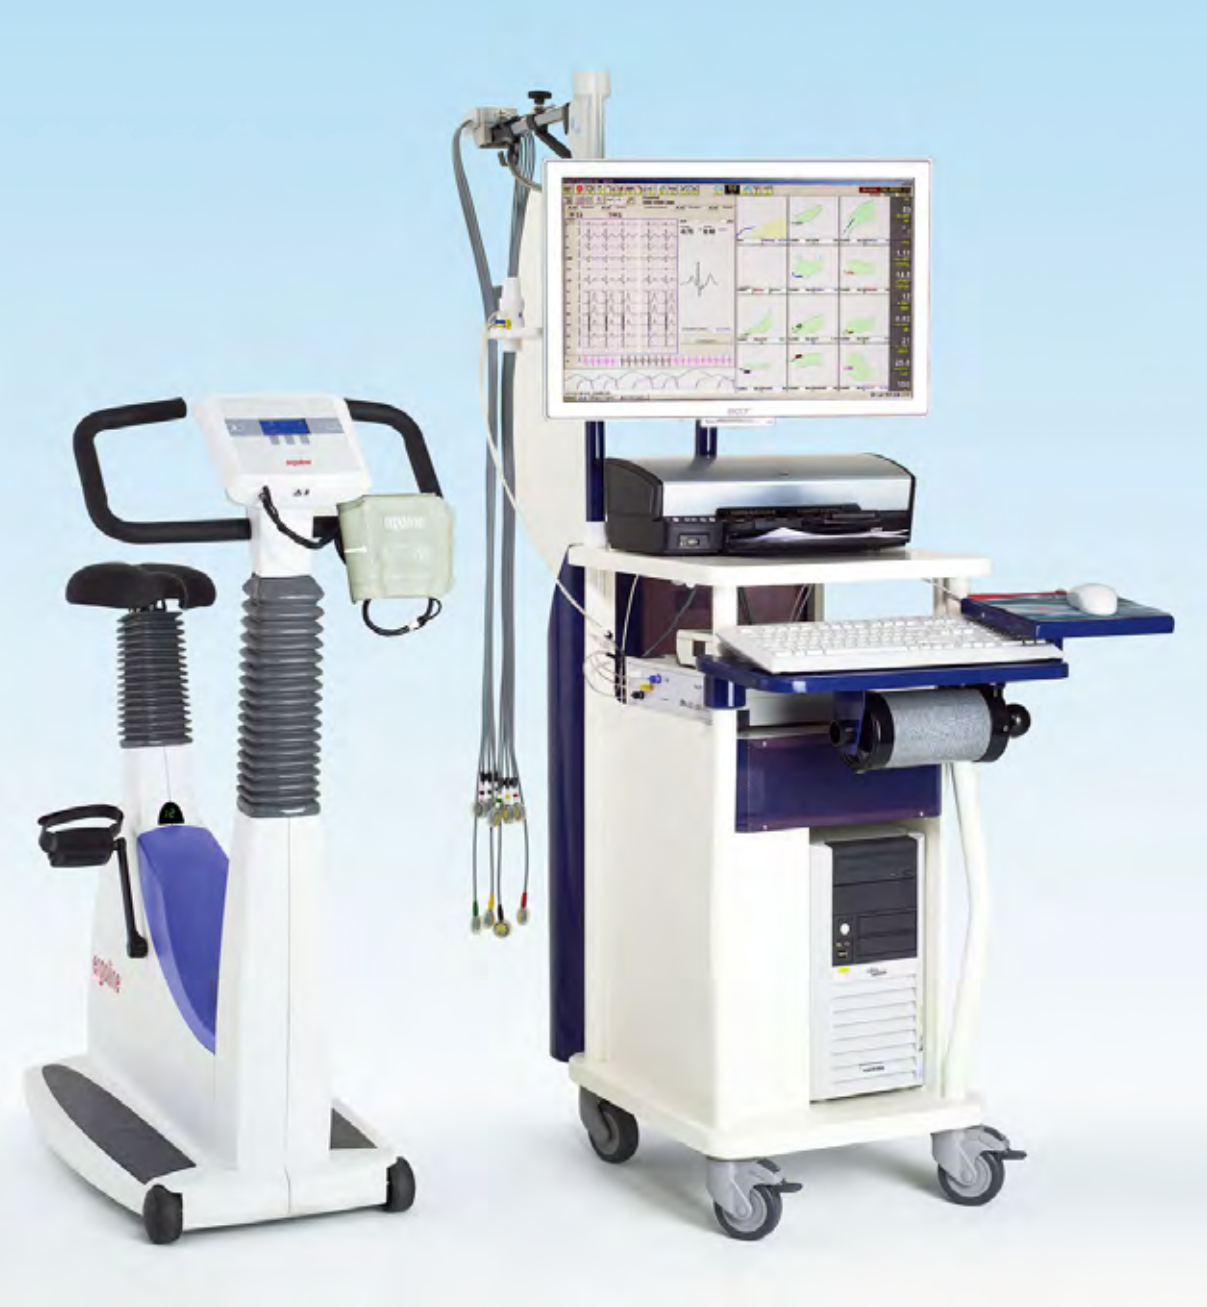
\includegraphics[width=\textwidth]{Figures/cpet-zan}
	\caption{ZAN-600 Cycle Erogmeter and CPET suite. (www.nspirehealth.com)}
	\label{fig:cpet-zan}
\end{figure}

CPET is composed of several components that involve measuring not only the response of the cardiac and respiratory system to exercise but the test also helps establish the adequacy of this response to sustain oxygen delivery to skeletal muscle as demand increases with increasing exercise. 

Cardiopulmonary exercise tests were performed in the Department of Respiratory Medicine at the Glasgow Royal Infirmary using the ZAN-600 CPET suite (nSpire Health, Longmont, CO 80501, USA). The equipment was calibrated regularly to the standards set by the manufacturer and currently published guidelines[]. All tests were performed by specialist respiratory physiologists. Suitable equipment for cardiopulmonary resuscitation were available in the department in case of unexpected problems. The department was situated within the main hospital premises and therefore was easily accessible to the hospital cardiac arrest team. All patients were fully informed of the steps involved in the procedure, the reasons for performing the test as well as the risks involved. 

Spirometry was performed in all patients prior to CPET. Capillary blood gases were measured in all patients after CPET. An electronically braked cycle ergometer was used to increase resistance to pedalling in preset increments. A tight-fitting face mask was placed on the patient covering the nose and the mouth. This allowed breath-by-breath gas analysis thus allowing measurement of several respiratory parameters as listed in table []. 12-lead electocardiogram was recorded at the same time. 

The test started with an initial 3-minute rest period to allow measurement of baseline parameters. This was followed by an incremental work-load test that involved the patient pedalling approximately at 60 revoultions per minute while the resistance to pedalling was gradually increased in preset increments. The test was terminated when patients reached volitional fatigue (maximal exercise tolerance), significant ischaemic changes on ECG or for other safety reasons. 

The parameters measured at spirometry are shown in Table \ref{table:spirometry} and those measured during cardiopulmonary exercise testing are shown in Table \ref{table:cpet_parameters} on p\pageref{table:cpet_parameters}.

\subsection{Measuring the Anaerobic Threshold}

\begin{figure}[htbp]
	\centering
	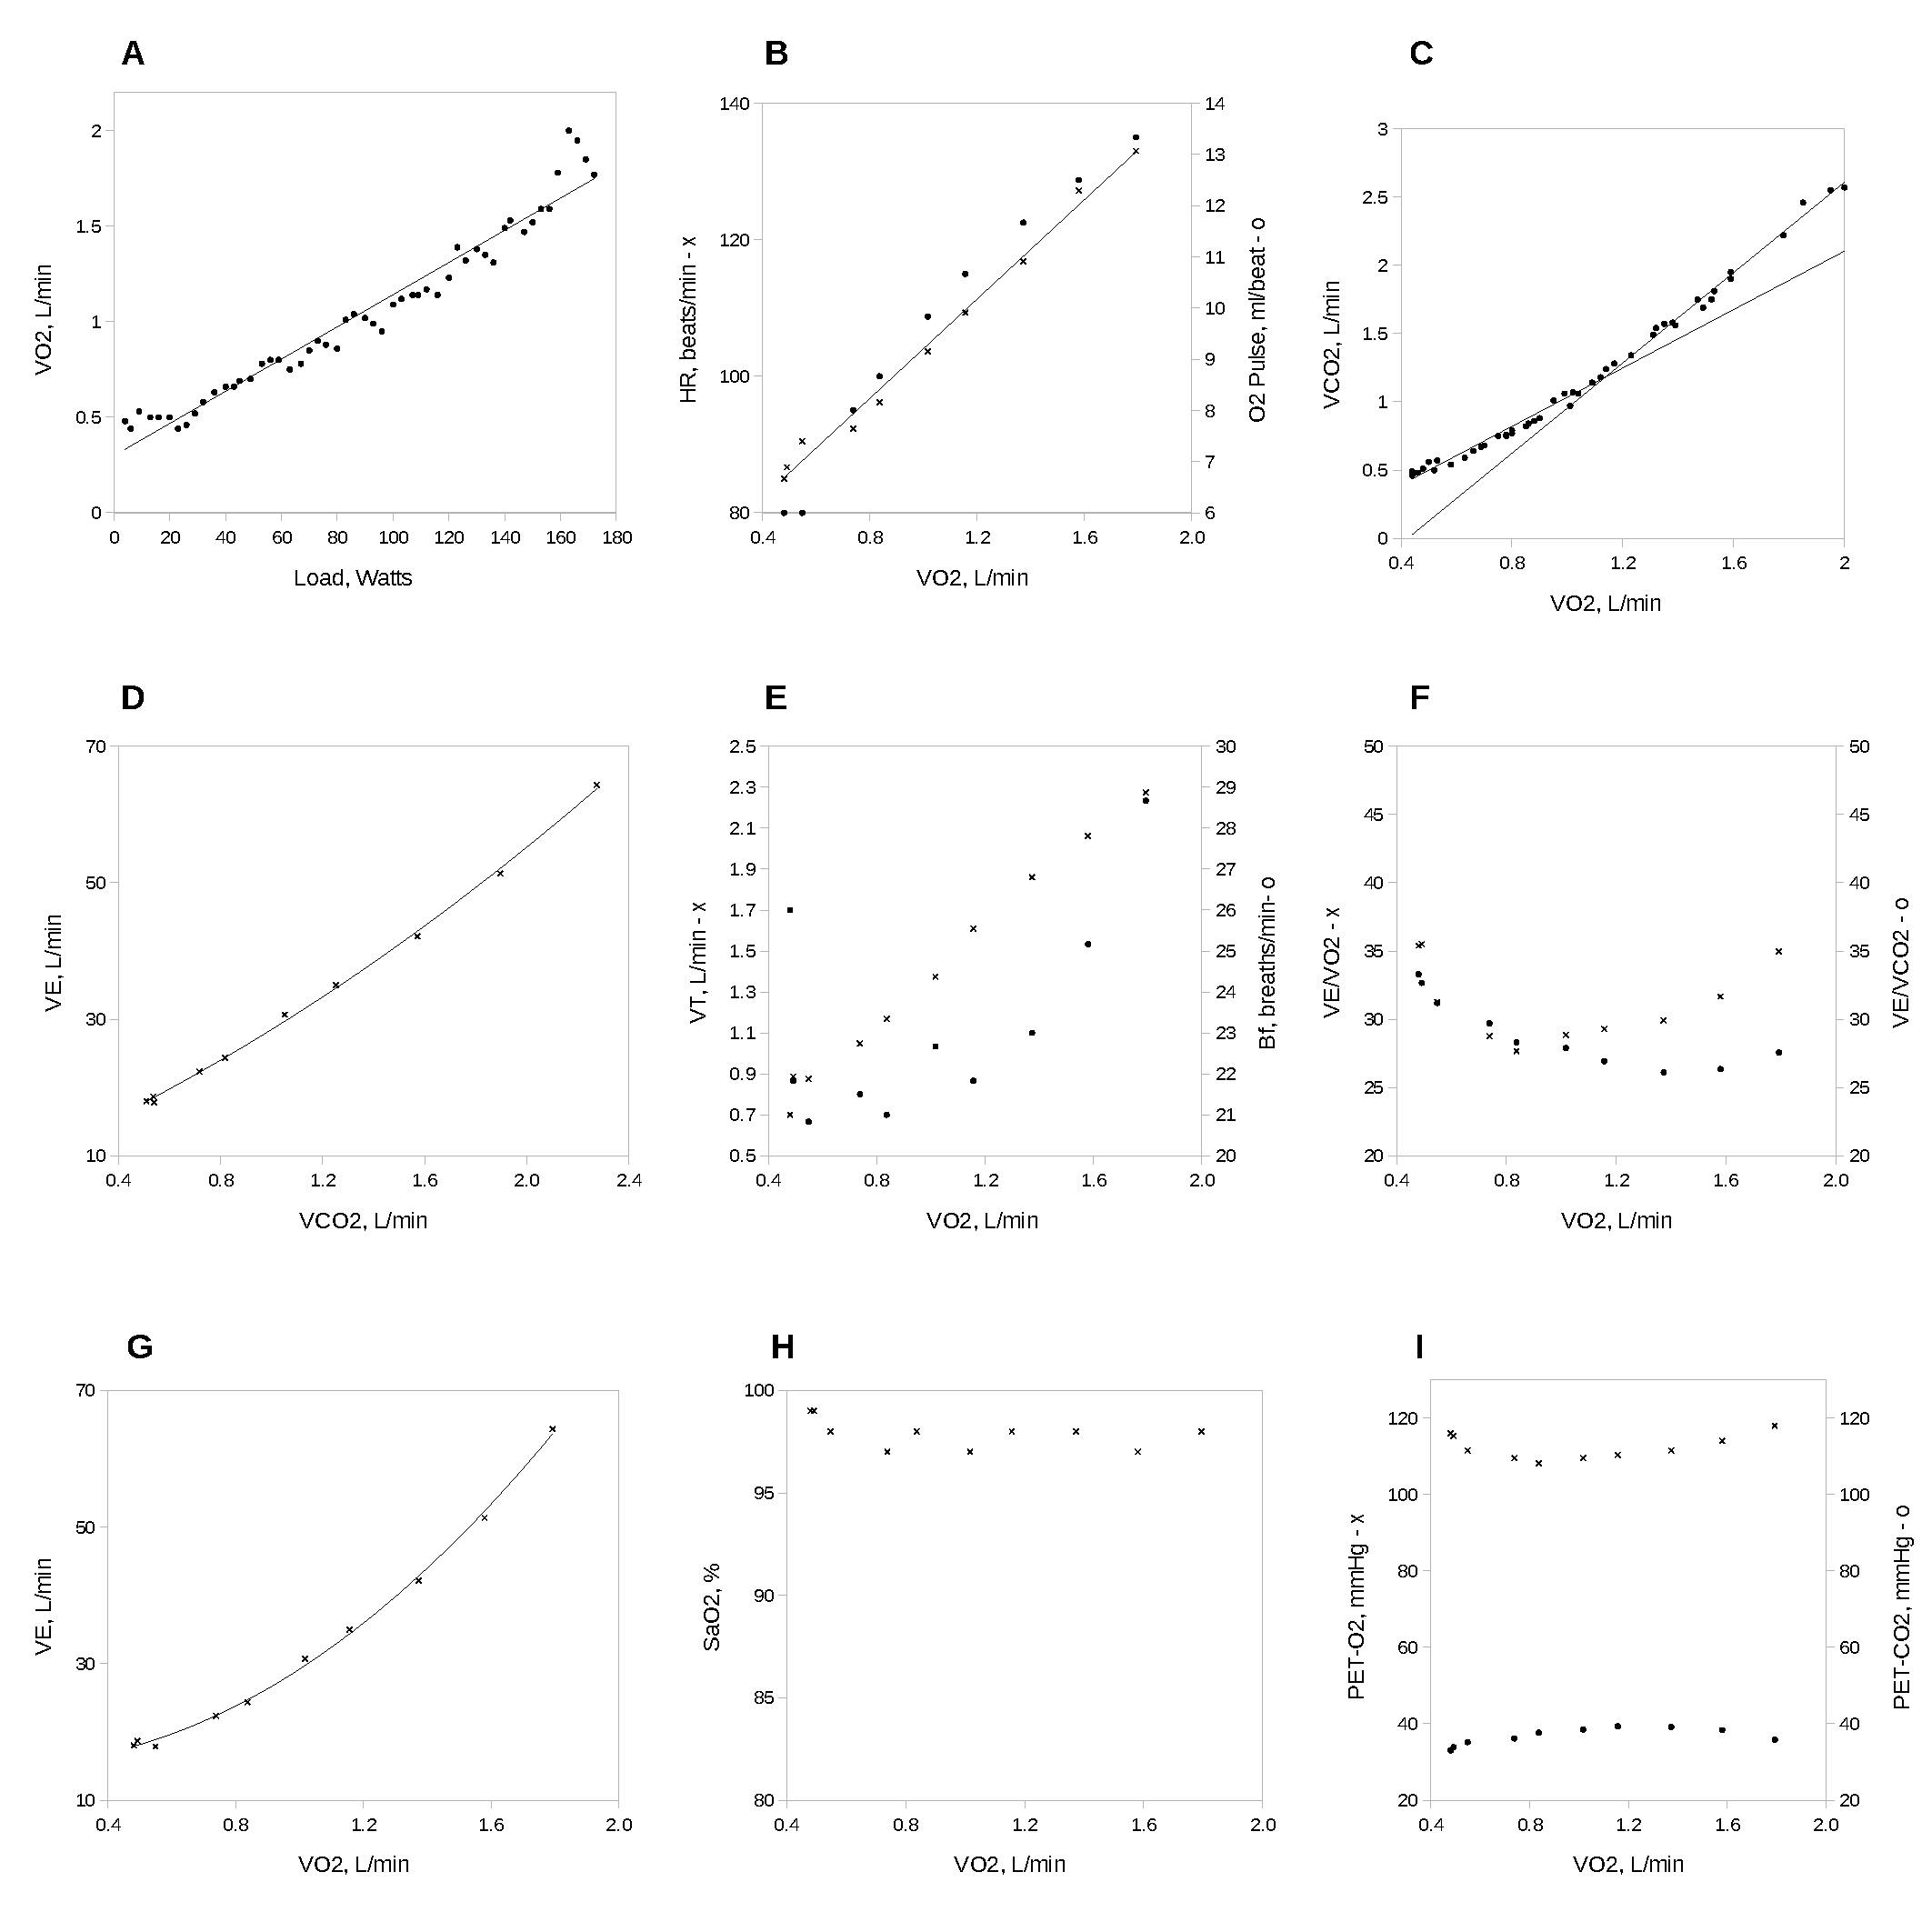
\includegraphics[width=\textwidth]{Figures/cpet_9panel.pdf}
	\caption{9-panel view of trending parameters during incremental cardiopulmonary exercise.}
	\label{fig:cpet_9panel}
\end{figure}

The anaerobic threshold (variously described as the lactate threshold or ventilatory threshold) is the point during exercise when oxygen demand by exercising skeletal muscle outstrips supply. Therefore, muscle tissues use anaerobic respiration to supplement aerobic respiration to continue generation of ATP. The resulting metabolic lactic acidosis is almost immediately compensated by the bicarbonate buffer as below: 
\begin{equation} \label{eq:bicarb_buffer}
	H^+ + HCO3^- \Longleftrightarrow H_2CO_3 \Longleftrightarrow H_2O + CO_2
\end{equation}
The resulting excess $CO_2$ is exhaled and is one of the many parameters measured during cardiopulmonary exercise testing. This transition from aerobic to anaerobic respiration may be determined using the V-slope method\parencite{sue_metabolic_1988} or the ventilatory equivalents method.\parencite{beaver_new_1986} Most centres, like ours, use both methods supplemented by information from a variety of other parameters to enable accurate determination of the anaerobic threshold as recommended by the American Thoracic Society/American College of Chest Physicians Statement on cardiopulmonary exercise testing.\parencite{society_ats/accp_2003}

The software presents a standard 9-panel view of trending plots of various parameters measured during incremental exercise. All of these trends are taken into consideration rather than any one particular parameter value in determining the overall outcome of the test. A sample 9-panel view derived from parameters belonging to one of the patients studied is shown in Figure \ref{fig:cpet_9panel}. The data used to generate these plots is included in Appendix \ref{AppendixCPETRawData}. 

\subsubsection{V-slope method}

\begin{figure}[htbp]
	\centering
	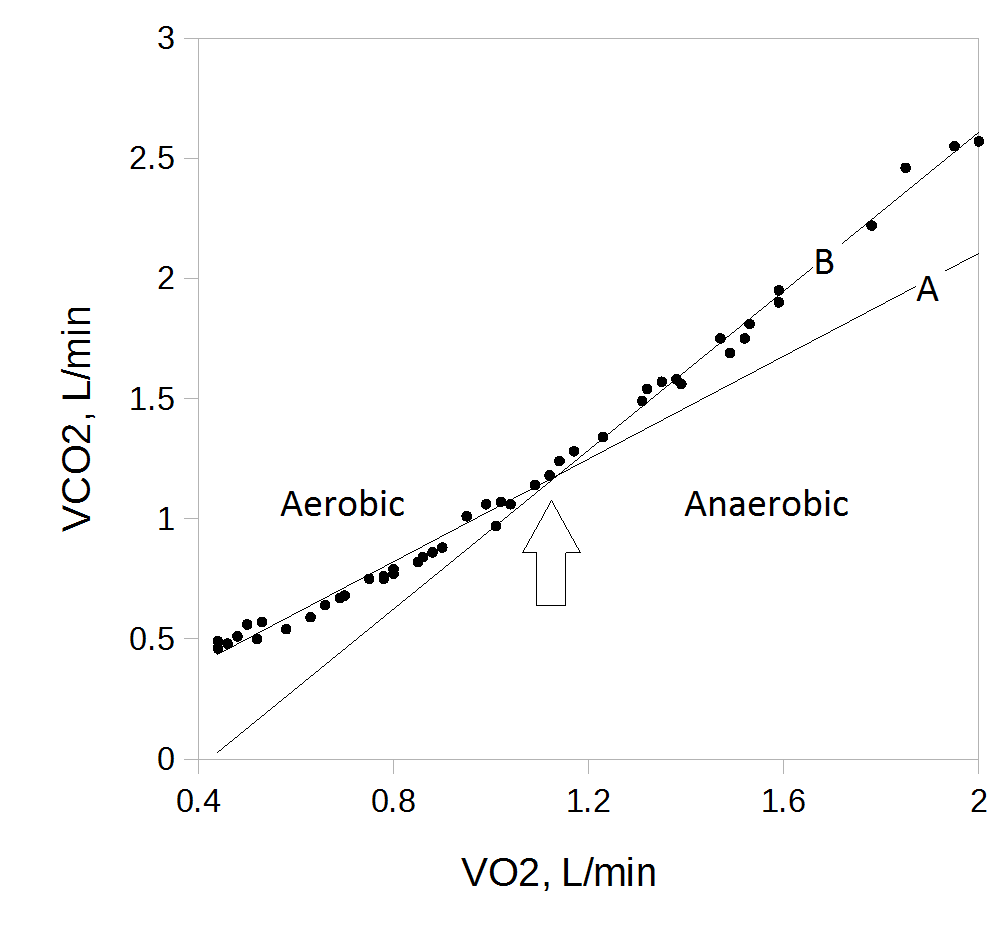
\includegraphics[width=\textwidth]{Figures/cpet_vslope}
	\caption{Determination of $\dot{V}_{O_2}$AT by the V-slope method.}
	\label{fig:cpet_vslope}
\end{figure}

During aerobic phase of exercise, $\dot{V}_{O_2}$ and $\dot{V}_{CO_2}$ share a linear relationship as shown in the left half of Figure \ref{fig:cpet_vslope} on p\pageref{fig:cpet_vslope}. However, as anaerobic respiration starts to supplement aerobic respiration, $\dot{V}_{CO_2}$ increases disproportionately to $\dot{V}_{O_2}$ as a direct result of the respiratory buffer described in equation \ref{eq:bicarb_buffer} on p\pageref{eq:bicarb_buffer}. This results in a distinct difference in the slope of the relationship between $\dot{V}_{O_2}$ and $\dot{V}_{CO_2}$ during aerobic exercise (Line A) versus during anaerobic exercise (Line B). The point at which the two slopes intersect is the anaerobic threshold and the $\dot{V}_{O_2}$ at this point in exercise is commonly referred to as the anaerobic threshold, $\dot{V}_{O_2}$AT or simply AT. 

\subsubsection{Ventilatory equivalents method}
The ventilatory equivalents method of determining $\dot{V}_{O_2}$AT involves plotting $\dot{V}_E/\dot{V}_{O_2}$
and $\dot{V}_E/\dot{V}_{CO_2}$ against time, exercise load or $\dot{V}_{O_2}$. The point at which $\dot{V}_E/\dot{V}_{O_2}$ increases while $\dot{V}_E/\dot{V}_{CO_2}$ stays the same or decreases is the anaerobic threshold and this can be seen in Fig. \ref{fig:cpet_9panel}F. Most respiratory physiologists including at our centre use both methods as well as other trends during exercise to determine the anaerobic threshold as well as its validity.


\section{Description of CPET Parameters}
\label{sec:cpx_parameters}
\begin{table}[p]
\centering
\caption{Parameters measured at spirometry.}
\label{table:spirometry}
\begin{tabular}{| m{2cm}  m{2cm}  m{7cm} |}
	\hline
	Parameter & Units  & Description                          \\ \hline
	FVC       & litres & Forced Vital Capacity                \\
	FEV1      & litres & Forced Expiratory Volume in 1 second \\
	FEV1/FVC  & \%     & Tiffeneau-Pinelli[1] index           \\ \hline
\end{tabular}

\vspace{2cm}


\caption{Common parameters measured at cardiopulmonary exercise testing.}
\label{table:cpet_parameters}
\begin{tabular}{| m{2cm}  m{2cm}  m{7cm} |}
	\hline
	Parameter & Units       & Description                                  \\ \hline
	\%peakVO2 & \%          & VO2 as a \% of predicted VO2Peak             \\
	Load      & Watts       & Exercise Workload                            \\
	VE        & litres/min  & Ventilatory Equivalent                       \\
	Vt        & litres      & Tidal volume                                 \\
	VO2       & litres/min  & Absolute Oxygen uptake/consumption           \\
	VO2/kg    & ml/(kg*min) & Corrected Oxygen uptake/consumption          \\
	VE/VO2    &             & Ventilatory Equivalent for O$_2$             \\
	VCO2      & litres/min  & Carbon-dioxide output                        \\
	VE/VCO2   &             & Ventilatory Equivalent for CO$_2$            \\
	RER       &             & Respiratory Exchange Ratio                   \\
	PETO2     & mmHg        & End Tidal O2                                 \\
	PETCO2    & mmHg        & End Tidal CO2                                \\
	O2Pulse   & ml/beat     & Oxygen pulse                                 \\
	HR        & beats/min   & Heart Rate                                   \\
	Bf        & /min        & Breathing Frequency                          \\
	P(A-a)O2  & mmHg        & Alveolar-arterial PO2 difference             \\
	Vd/Vt     &             & Physiologic dead space-to-tidal volume ratio \\
	SBP       & mmHg        & Systolic blood pressure                      \\
	DBP       & mmHg        & Diastolic blood pressure                     \\
	O2sat     & \%          & Oxygen saturation                            \\ \hline
\end{tabular}

\end{table}


\subsection{Exercise Load}
The most common form of cardiopulmonary exercise testing for clinical use involves a cycle ergometer with steadily increasing resistance delivered through electric braking. This allows accurate measurement of work load in Watts. The relationship between $\dot{V}_{O_2}$ and work rate is usually linear and the slope of this relationship is independent of sex, age or height. An abnormality in this relationship is usually due to cardiopulmonary or circulatory causes.

\subsection{Minute Ventilation, $\dot{V}_E$}
Minute ventilation or respiratory minute volume is the volume of air that is inhaled/expired in a minute.
\begin{equation} \label{eq:VE=VTxBf}
	\dot{V}_E = \dot{V}_T \times Bf
\end{equation}
where $\dot{V}_T$ = Tidal Volume and $Bf$ = Breathing Frequency.

Increasing $\dot{V}_E$ is one of the main mechanisms involved in increasing oxygen delivery during exercise. It is also an important factor in clearing $CO_2$ from the blood.

\subsection{Oxygen Uptake, $\dot{V}_{O_2}$}

$\dot{V}_{O_2}$ or oxygen uptake is measured breath-by-breath using digital analysis of the inspired and expired gases. This is then averaged, usually over time, to smooth-out any signficant breath-by-breath variation. $\dot{V}_{O_2}$ increases with increasing work load and is influenced by several factors that have a role in the transport and utilisation of oxygen. These may be broadly classified as cardiac, pulmonary, circulatory and tissue factors. Some of the factors are encompassed in the following formula for $\dot{V}_{O_2}$.
\begin{equation} \label{eq:oxygen_consumption}
	\dot{V}_{O_2} = CaO_2 \times Cardiac\ Output
\end{equation}
where $CaO_2$ is $O_2$ content per ml of blood and is defined by,
\begin{equation} \label{eq:CaO2}
	CaO_2 = Haemoglobin \times 1.34 \times SaO_2
\end{equation}
and
cardiac output, the primary cardiac factor that influences $\dot{V}_{O_2}$, is:
\begin{equation} \label{eq:CO=SVxHR}
	Cardiac\ Output = Stroke\ Volume \times Heart\ Rate
\end{equation}
Stroke volume is in turn influenced by ventricular function and end-diastolic volumes. The heart rate response to exercise is discussed in section \ref{sec:heart_rate} on p\pageref{sec:heart_rate}.

Pulmonary gas exchange plays an important role in the oxygenation of blood and removal of $CO_2$ and is influenced by numerous factors, the detailed discussion of which is beyond the scope of this chapter. However, ventilation, pulmonary blood flow, gas-exchange across the alveolar membrane and ventilation-perfusion mismatches (V/Q mismatch) all play an important role in determining the response of the lungs to exercise.

The quality of the peripheral circulation, both anatomical and its physiologic response to exercise which involves redistribution of blood flow to exercising muscle, has an important role in increasing availability of oxygen. The oxygen carrying capacity of blood determined by haemoglobin concentration, its saturation and the $O_2$ dissociation curve as well as the ability of tissues to extract and utilise oxygen are equally important factors that influence $\dot{V}_{O_2}$.

\subsection{Oxygen Pulse, $O_2Pulse$}
Oxygen pulse is defined as the oxygen uptake per heart beat.
\begin{equation} \label{eq:oxygen_pulse}
	O_2Pulse = \frac{\dot{V}_{O_2}}{Heart\ rate}
\end{equation}
While some authors have suggested that oxygen pulse may be a surrogate for stroke volume others disagree. The clinical application of oxygen pulse in surgical patients remains unclear.

\subsection{Respiratory Exchange Ratio, RER}
The ratio of $\dot{V}_{CO_2}/\dot{V}_{O_2}$ is called the Respiratory Exchange Ratio. An RER greater that 1.0 may be caused either by lactic acidosis or due to hyperventilation. The RER is also a marker of the fuel being used for metabolism with RER less than 1.0 indicating mixed fuel source in the form of carbohydrate and fat while an RER of 1.0 or greater indicates a primarily carbohydrate source.

\subsection{Ventilatory Equivalent for $O_2$ and $CO_2$, $\dot{V}_E/\dot{V}_{O_2}$, $\dot{V}_E/\dot{V}_{CO_2}$}
The changes in $\dot{V}_E/\dot{V}_{O_2}$ and $\dot{V}_E/\dot{V}_{CO_2}$ during exercise provide valuable information regarding the ventilatory response to exercise. Both $\dot{V}_E/\dot{V}_{O_2}$ and $\dot{V}_E/\dot{V}_{CO_2}$ tend to decrease initially during exercise. However, as the anaerobic threshold is passed, $\dot{V}_E/\dot{V}_{O_2}$ starts increasing before $\dot{V}_E/\dot{V}_{CO_2}$. This change in direction is yet another method to confirm the anaerobic threshold.  $\dot{V}_E/\dot{V}_{CO_2}$ eventually starts increasing as respiratory compensation of metabolic acidosis results in increased $\dot{V}_E$.

\subsection{End-tidal $O_2$ and $CO_2$, $P_{ET_{O_2}}$, $P{ET_{CO_2}}$}
$PET_{O_2}$ and $PET_{CO_2}$ are the partial pressures of $O_2$ and $CO_2$ at the end of an exhaled breath and are closely related to PaO2 and PaCO2 respectively. $P{ET_{CO_2}}$ is dependent on pulmonary gas-exchange which is in turn influenced by the right ventricular output, pulmonary blood flow and alveolar gas exchange. The changes in $P_{ET_{O_2}}$ and $P{ET_{CO_2}}$ during exercise help identify ventilation-perfusion mismatch as well as hyperventilation.

\subsection{Heart Rate, HR}
\label{sec:heart_rate}
The heart rate response during exercise in healthy individuals is a linear function of $\dot{V}_{O_2}$ increasing linearly with increasing work load and increasing $\dot{V}_{O_2}$. The difference between the predicted peak heart rate and the observed peak heart rate is called the Heart Rate Reserve or HRR. Failure to achieve the predicted peak heart rate or a wide HRR may be due to cardiac disease or due to medication used to treat cardiovascular disorders such as beta-blockers or calcium-channel blockers. This information in conjunction with 12-lead ECG evidence of ischaemia provides undeniable evidence of primary cardiac dysfunction.

\subsection{Breathing frequency, $B_f$}
In healthy individuals, breathing frequency is one of the most important respiratory responses to exercise in order to increase oxygen uptake. However, a variety of respiratory disorders including obstructive disorders such as chronic obstructive pulmonary disease or restrictive disorders such as interstitial lung disease can impair this response. Morbidly obese patients may also have additional restrictions on respiratory response due to their body habitus. On the other hand, hyperventilation in an otherwise healthy patient may make interpretation of the results difficult although the analysis of trends in other parameters such as $P_{ET_{O_2}}$ and $P{ET_{CO_2}}$ aids in the diagnosis of hyperventilation versus true respiratory problems.

\section{Role of CPET in preoperative assessment}
\label{sec:cpx_roleInAssessment}
\subsection{General Surgery}

Several studies over the past 2 decades have established the value of cardiopulmonary exercise testing in patients, especially elderly, undergoing major abdominal surgery. Older and co-workers conducted a prospective study of 187 patients over the age of 60 undergoing major abdominal surgery. All patients underwent a symptom-limited exercise test on a cycle ergometer with real-time 12-lead ECG monitoring. The average $\dot{V}_{O_2}$ across all patients was 12.4 ml/min/kg. There were a total of 11 deaths related to cardiovascular causes (5.9\%) and 3 deaths due to non-cardiovascular causes. They reported that 10 out of the 11 deaths due to cardiovascular causes occurred in patients with $\dot{V}_{O_2}AT<11$ml/kg/min (n=55) while only one patient in the group with $\dot{V}_{O_2}AT\geq11$ml/kg/min (n=132) died of cardiovascular complications (18\% vs 0.8\%, $p<0.001$). Eight out of the 10 patients in the low $\dot{V}_{O_2}$AT group who died also had evidence of myocardial ischaemia ($p<0.01$).\parencite{older_preoperative_1993}
 
In a later, larger prospective study of 548 patients who underwent major abdominal surgery including colorectal and abdominal aneurysm surgery, they used a risk stratification system that combined $\dot{V}_{O_2}AT<11$ml/kg/min, $\dot{V}_E/\dot{V}_{CO_2}>35$ and evidence of myocardial ischaemia during exercise. High risk patients ($\dot{V}_{O_2}AT<11$ml/kg/min, n=153) were admitted to intensive care after surgery and had a mortality due to cardiovascular causes of 4.6\%. Moderate risk group ($\dot{V}_{O_2}AT>11$ml/kg/min and either $\dot{V}_E/\dot{V}_{CO_2}>35$ or evidence of myocardial ischaemia, n=115) was managed in the high dependency unit after surgery and had a cardiovascular mortality of 1.7\%. Low risk patients (with none of the risk factors mentioned above, n=280) were managed on the general surgical ward with no cardiovascular mortality.\parencite{older_cardiopulmonary_1999} Subsequent literature reviews by Older and co-workers have emphasised the value of cardiopulmonary exercise testing in risk assessment as well as optimising perioperative care in the high-risk surgical patient. \parencite{older_preoperative_2000, older_clinical_2004, older_preoperative_2005}

These findings have since been replicated in several other studies although the threshold value of $\dot{V}_{O_2}$AT as well as the inclusion of other CPET parameters to attribute risk differ in these studies. Hightower and co-workers studied 32 patients over the age of 18 undergoing a variety of major elective abdominal surgery. In this heterogenous cohort, they reported that the percent predicted anaerobic threshold achieved $<$ 75\%, heart rate at the anaerobic threshold and the heart rate response from rest to anaerobic thresold were all independently associated with postoperative morbidity. While it is difficult to extrapolate results from this small heterogenous cohort to the general surgical population, it would appear that other cardiopulmonary exercise test parameters may have a role in predicting risk in these patients.\parencite{hightower_pilot_2010}

Snowden and coworkers reported in a study of 171 patients of who 123 underwent surgery, that $\dot{V}_{O_2}AT<10.1$ ml/kg/min was associated with not only cardiovascular complications but also with other complications including pulmonary, renal, gastrointestinal, infective and haematological complications. One of the strengths of this study was the fact that the clinicians treating these patients were blinded to the results of preoperative cardiopulmonary exercise testing results thus avoiding management bias. They also included other cardiopulmonary exercise test parameters such as $\dot{V}_{O_2}$Peak and $\dot{V}_E/\dot{V}_{CO_2}$ at the anaerobic threshold in addition to $\dot{V}_{O_2}$AT in their analysis and showed that $\dot{V}_{O_2}$AT was more predictive of postoperative morbidity than POSSUM derived morbidity, cardiac risk scoring index or a validated activity questionnaire. However, this study also included a heterogenous cohort of diseases including vascular, pancreatic and hepatobiliary disorders and sarcomas.\parencite{snowden_submaximal_2010}

In a study of 847 patients undergoing elective abdominal surgery for colorectal disease, bladder or renal cancer, Wilson and co-workers found that $\dot{V}_{O_2}AT<11$ ml/kg/min in patients with no documented history of cardiac risk factors was associated with a relative risk of mortality of 10.0 (95\% CI 1.7-61.9).\parencite{wilson_impaired_2010} This emphasises the value of cardiopulmonary exercise testing in diagnosing sub-clinical or previously undiagnosed (and untreated) cardiovascular and respiratory disease. Moreover, 90-day survival was also better in patients with better aerobic capacity ($\dot{V}_{O_2}AT>11$ ml/kg/min and $\dot{V}_E/\dot{V}_{CO_2}<34$) {a}nd in patients without ischaemic heart disease. It would appear therefore that This appears to suggest that aerobic capacity influenced not only postoperative outcomes but also medium term survival after patients left hospital.

\subsection{Oesophago-gastric and bariatric surgery}
In a retrospective study involving 91 patients who underwent curative oesophagectomy with 3-field lymphadenectomy via a
right thoracotomy for squamous cell carcinoma of the thoracic oesophagus between 1991 and 1995, Nagamatsu and co-workers reported that $\dot{V}_{O_2}max/m^2<800$ml/min/m$^2$ predicted cardiopulmonary complications.\parencite{nagamatsu_preoperative_2001} They also reported that $\dot{V}_{O_2}AT/m^2$ and routine spirometry did not predict cardiopulmonary complications. They recommended that in patients with $\dot{V}_{O_2}max/m^2<800$ml/min/m$^2$, surgical treatment be modified either into a 2-stage procedure or a trans-hiatal procedure avoiding a thoracotomy where possible.

Cardiopulmonary exercise testing has also been useful in predicting short-term complications after bariatric surgery. McCullough and co-workers defined a composite primary outcome measure that included myocardial infarction, unstable angina, deep vein thrombosis, pulmonary embolism, renal failure, stroke and death and applied this in a cohort of 109 consecutive patients who underwent Roux-en-Y gastric bypass surgery. This composite adverse outcome was more likely in patients with high BMI ($>45$) and low $\dot{V}_{O_2}$Peak ($<15.9 ml/kg/min$). In fact, patients with neither of these two risk factors had no complications after surgery. They also observed a significant negative relationship between BMI and $\dot{V}_{O_2}$ ($p<0.0001$) and age($p<0.0001$). Poor aerobic capacity was also associated with the presence of diabetes and hypertension suggesting further evidence of the metabolic cost of obesity in these patients.\parencite{mccullough_cardiorespiratory_2006}

However, Forshaw and co-workers reported that cardiopulmonary exercise testing was of limited use in predicting complications after oesophagectomy.\parencite{forshaw_is_2008} They studied 78 patients undergoing either trans-hiatal (n=39) or trans-thoracic (n=39) oesophagectomy. They evaluated several thresholds for both $\dot{V}_{O_2}$Peak and $\dot{V}_{O_2}$AT and found no useful correlation with cardiopulmonary complications, non-cardiopulmonary complications, length of stay in critical care or in hospital. While $\dot{V}_{O_2}$Peak was significantly lower in patients who developed postoperative cardiopulmonary complications, receiver-operator characteristics (ROC) analysis did not identify a clinically useful threshold that would stratify patients into different risk groups. They postulated that the fact that post-oesophagectomy complications such as anastomotic leak or sepsis often happen within the thorax and are not necessarily due to cardiopulmonary dysfunction, preoperative cardiopulmonary exercise testing may not have identified these patients. Older and Hall, the pioneers of cardiopulmonary exercise test in surgical patients, also raise this issue in their letter to the authors of the above study. \parencite{hall_cardiopulmonary_2009}

\subsection{Vascular Surgery}
The earliest report of the application of cardiopulmonary exercise test in elective abdominal aortic aneurysm surgery was by Nugent and co-workers in 1998. They reported on cardiopulmonary exercise testing using a treadmill in 36 patients undergoing elective abdominal aortic aneurysm surgery. They found no difference in the $\dot{V}_{O_2}$Peak in patients who developed complications versus those who did not (18.6 vs 2.8 ml/kg/min, p$>$0.05). However, they reported that in the 4 patient who were denied surgery as they were deemed medically unfit, $\dot{V}_{O_2}$Peak was less than 20 ml/kg/min. However, this threshold did not discriminate patients who developed complications and the authors concluded that cardiopulmonary exercise testing should not be used on its own to guide clinical management of these patients.\parencite{nugent_cardiopulmonary_1998}

However, cardiopulmonary exercise testing has been reported to predict 2-year survival in patients undergoing elective aortic aneurysm surgery. Carlisle and Swart reported that a Revised Cardiac Risk Index (RCRI) score $>1$ in combination with a $\dot{V}_E/\dot{V}_{CO_2}>42$ was associated with a 2-year survival rate of 55\% while the 2-year survival rate was 97\% if neither risk factor was present. $\dot{V}_{O_2}$AT was not a predictor of survival in multi-variate analysis in this study.\parencite{carlisle_mid-term_2007}

While studies have reported that repeated cardiopulmonary exercise testing provides reproducible results in patients with abdominal aortic aneurysm and preoperative exercise regimens are safe and effective at increasing aerobic capacity in patients awaiting surgery, there is no published literature on the association between cardiopulmonary exercise testing and postoperative complications in patients undergoing vascular surgery. %True as of 2010. There are several papers post 2010. 

\subsection{Liver Transplantation}
Peak $\dot{V}_{O_2}<60\%$ predicted and $\dot{V}_{O_2}AT<50\%$ predicted have been reported to be associated with increased 100-day mortality in patients undergoing liver transplantation. In patients with cirrhosis awaiting hepatic transplantation, reduced aerobic capacity may not only be due to primary cardiorespiratory insufficiency but may also be due to the secondary effects of hepatic dysfunction itself. These include cirrhotic cardiomyopathy, hepatopulmonary syndrome and decreased peripheral oxygen utilisation due to cirrhotic myopathy.\parencite{epstein_aerobic_2004} This is further supported by the fact that patients who undergo liver transplantation have been shown to have improved aerobic capacity a year after surgery. \parencite{iscar_functional_2009} However, there is very little other evidence of the application of cardiopulmonary exercise testing in patients undergoing major hepato-pancreato-biliary surgery or liver transplantation.

\subsection{Thoracic Surgery}
The role of cardiopulmonary exercise testing in patient undergoing non-cardiac thoracic surgery has been well established for over a decade. In a recent meta-analysis of 14 studies, Benzo and co-workers reported on 955 patients who underwent cardiopulmonary exercise tests as part of their preoperative work-up before lung resection for cancer. $\dot{V}_{O_2}$Max (ml/kg/min), $\dot{V}_{O_2}$Max (\% predicted), maximum exercise load achieved (Watts) and FEV1 (\% predicted) were all significantly higher in patients who recovered with no postoperative complications. They also found that the mean $\dot{V}_{O_2}$Max in patients who did not develop complications was approximately 20 ml/kg/min and the mean $\dot{V}_{O_2}$Max in patients who developed complications was 15 ml/kg/min across all studies. This would suggest that cardiopulmonary exercise testing can offer clinically useful thresholds across different populations that can be used to risk stratify patients.\parencite{benzo_complications_2007}

The 2$^nd$ edition of the American College of Chest Physicians' Evidence-Based Clinical Practice Guidelines for the 'Physiologic evaluation of the patient with lung cancer being considered for resectional surgery' recommends that patients with a low $\dot{V}_{O_2}$Max ($<10$ ml/kg/min) or with low $\dot{V}_{O_2}$Max ($<15$ ml/kg/min) associated with other risk factors on spirometry and cardiopulmonary exercise testing should be counselled about non-operative treatment options and non-standard surgery as the risk of perioperative death and cardiopulmonary complications was very high. The 1C grading of this recommendation not only represents the observational nature of most of the studies it is based on but also that such observational evidence is sufficiently consistent\parencite{benzo_complications_2007} to make a strong recommendation.\parencite{colice_physiologic_2007}

\clearpage

\section{Systemic inflammation and outcome}
\label{sec:intro_systemic_inflammation_outcome}

%Preop inflammation - short-term and long-term outcomes
%Postop inflammation -> complications -> long-term ouctomes
%Possible mechanisms behind poor outcomes

The host inflammatory response to cancer, comorbidity and surgical trauma has been known to influence both short-term and long-term outcomes after major cancer surgery. Moreover, postoperative complications have been reported to be associated with poorer oncologic outcomes and cancer-specific survival in patients undergoing potentially curative surgery for cancer. The complex interactions between pro-inflammatory cytokines and anti-inflammatory cytokines at different phases during the perioperative period further impact upon the incidence of complications as well as survival.

\subsection{Measuring systemic inflammation}
Numerous tests are available to not only measure systemic inflammation in general but also to quantify the various components of the inflammatory response. The most commonly employed measures in the clinical setting are the serum levels of C-reactive protein (CRP)and the differential leucocyte count. 

One of the earliest reports on the use of CRP to predict cancer-specific survival was by McMillan and co-workers in 1995 when they reported that an elevated CRP 4 months after curative resection for colorectal cancer was associated with earlier recurrence.\parencite{mcmillan_prospective_1995} The modified Glasgow Prognostic Score (mGPS)\parencite{elahi_score_2004} is based on a combination of C-reactive protein and serum albumin and is outlined in Table \ref{table:mGPS}. Since its introduction, mGPS has been validated in over a hundred studies looking at several thousand patients with a wide-range of cancers and an increasing score is associated with poorer long-term survival in patients with operable as well as inoperable cancers.

\begin{table}[h]
	\centering
	\caption{The modified Glasgow Prognostic Score}
	\label{table:mGPS}
	\begin{tabular}{c c c}
		mGPS & CRP (mg/dL) & Albumin  (mg/dL) \\ \hline
		 0   & $\leq 10$   & $\geq 35$        \\
		 1   & $> 10$      & $\geq 35$        \\
		 2   & $> 10$      & $< 35$
	\end{tabular}
\end{table}

\subsection{Systemic inflammation and long-term survival}
Systemic inflammation is associated with poorer survival in patients undergoing potentially curative surgery for pancreatic cancer \parencite{jamieson_systemic_2005,clark_preoperative_2007,bhatti_preoperative_2010} as well as in patients with inoperable pancreatic cancer.\parencite{glen_evaluation_2006} Patients with ductal adenocarcinoma of the head of the pancreas undergoing potentially curative resection survived for a median of 21.5 months if their CRP was $\leq$ 10 mg/dl a month after their surgery but only 8.4 months if their CRP remained persistently elevated at over 10 mg/dl approximately a month after their operation.\parencite{jamieson_systemic_2005} Similar findings have been reported in cancers involving other organs using both the mGPS and other scores such as the neutrophil-lymphocyte ratio (NLR). A selection of these studies are presented in Table %Create new table here for this.

\subsection{Systemic inflammation and postoperative complications}

Abnormalities of systemic inflammatory processes present as a continuum that starts in the preoperative phase possibly as a consequence of underlying comorbid illnesses, presence of cancer, or an abnormality of the immune system or a due to a combination of all of these factors. Surgical trauma in such 'primed' patients results in a cascade of events that trigger several inflammatory pathways that have now shown to have a direct impact not only on the incidence of postoperative complications but also on cancer recurrence and long-term survival.

\subsubsection{Preoperative systemic inflammation}
Elevated levels of interleukin-6, alpha-1 antitrypsin and CRP and decreased levels of albumin and prealbumin before surgery have been reported to be associated with a more exaggerated postoperative systemic inflammatory response and infectious complications after major abdominal surgery.\parencite{haupt_association_1997}

Preoperative systemic inflammation has been reported to be associated with infectious complications in patients undergoing potentially curative surgery for colorectal cancer.\parencite{moyes_preoperative_2009} In a study of 455 patients, Moyes and coworkers reported that an elevated preoperative modified Glasgow Prognostic Score (\ref{table:mGPS}) was associated with increased incidence of infectious complications in patients undergoing elective as well emergency colorectal cancer surgery. They postulated that several mechanisms may have a role including disregulation of cell-mediated immunity, impaired T-lymphocyte response, disorders in the complement pathway and possibly due to loss of lean tissue and protein as a consequence of systemic inflammation. Preoperative mGPS has also been shown to predict postoperative morbidity in patients undergoing oesophageal resection for cancer.\parencite{vashist_glasgow_2010} 

\subsubsection{Postoperative systemic inflammation}
An exaggerated and persistent systemic inflammatory response in the early postoperative period is associated with an increased incidence of complications. One of the earliest studies comparing several 'acute-phase proteins' and their role in predicting postoperative complications reported that in patients who developed surgical inflammatory complications, CRP remained elevated after the third postoperative day while other acute-phase proteins such as ceruloplasmin and alpha-1 antitrypsin where not useful in monitoring the postoperative course.\parencite{fischer_quantitation_1976} 

Further studies have established the value of monitoring trends in serum CRP levels in predicting complications after both elective and emergency surgery.\parencite{mustard_c-reactive_1987}

In a study of 383 patients undergoing elective rectal cancer surgery with primary anastomosis, Welsch and co-workers reported that persistently raised CRP level over 140 mg/L after the third/fourth postoperative day was associated with anastomotic leak.\parencite{welsch_c-reactive_2007} They also reported in a separate study of 688 patients undergoing pancreatic resection with pancreaticojejunostomy for neoplastic disease or chronic pancreatitis, that persistently elevated CRP levels greater than 140 mg/L on the fourth postoperative day was associated with increased incidence of complications. 

Similar findings have been reported after elective colorectal surgery\parencite{ortega-deballon_c-reactive_2010, woeste_increased_2010}, oesophago-gastric surgery\parencite{dutta_persistent_2011}, spinal surgery\parencite{meyer_c-reactive_1995,mok_use_2008}, neurosurgery\parencite{al-jabi_value_2010}, simultaneous pancreas-kidney transplantation\parencite{wullstein_high_2004}, stem-cell transplantation\parencite{mcneer_early_2010} and paediatric surgery\parencite{laporta_baez_c-reactive_2011}.

While CRP level between the third and fifth postoperative day has been reported to be most predictive of complications,  the complications themselves do not become clinically apparent until a later in the postperative course, ofter after the fifth postoperative period. This has led some authors to postulate that the elevated CRP levels may in fact be due to an abnormally modulated postoperative inflammatory response resulting in an initial exaggerated systemic inflammatory response syndrome (SIRS) followed by a compensatory anti-inflammatory response syndrome (CARS). 

\subsubsection{Compensatory Anti-inflammatory Response Syndrome (CARS)}
The compensatory anti-inflammatory response syndrome is characterised by several features including reduction in lymphocyte numbers by apoptosis, decreased responsiveness of monocytes to cytokines, reduced number of human leukocyte antigen presenting receptors on monocytes, expression of cytokines that suppress Tumour Necrosis Factor (TNF) and clonal anergy.

In their seminal work on the role of SIRS and CARS in the pathogenesis of sepsis and organ dysfunction, Bone and co-workers described a state of 'immunologic dissonance' where a 'pre-primed' immune system may result in an inappropriate, out-of-balance massive pro-inflammatory response which is followed by a proportionately large compensatory anti-inflammatory response that leaves the patient immunosuppressed and prone to further organ dysfunction, infections and death. \parencite{bone_sepsis:_1997, bone_immunologic_1996} It is very likely that similar mechanisms are involved in surgical patients except that the initial stressor in this case is surgical trauma rather than a bacterial infection as in sepsis. 

This form of 'immunoparalysis' was first described in patients after major trauma with tissue damage \parencite{abraham_effects_1985,bandyopadhyay_negative_2007} or after haemorrhage on its own without associated tissue trauma. \parencite{stephan_hemorrhage_1987} In a detailed review of the mechanisms underlying the compensatory anti-inflammatory response syndrome, Ward and coworkers describe SIRS and CARS to be mirror images suggesting that a disproportionately high SIRS is followed by a period of immunosuppression that leaves the patient prone to further complications.\parencite{ward_compensatory_2008}

Patients who developed infectious complications after major cancer surgery had higher levels of interleukin-10 (IL-10), an anti-inflammatory cytokine and marker of the compensatory anti-inflammatory process.\parencite{mokart_early_2002} Major surgery and the associated surgical trauma is associated with elevated levels of IL-10 which in turn is associated with increase in lymphocyte apoptosis \parencite{delogu_interleukin-10_2001}, reduced monocyte expression of HLA-DR antigens \parencite{klava_interleukin-10._1997} and a blunted response to endotoxins \parencite{ogata_role_2000, kawasaki_surgical_2001}, all considered to be key features of a compensatory anti-inflammatory response syndrome. 

Yamaguchi and co-workers compared the levels of pro- and anti-inflammatory cytokines in patients undergoing cholecystectomy versus patients undergoing trans-thoracic oesophagectomy. They reported that the initial inflammatory phase was followed by an immunosuppressive phase that started around the seventh postoperative day in patients undergoing oesophagectomy. However, patient who underwent underwent an open cholecystectomy did not experience this immunosuppressive phase, leading them to postulate that the degree of immunosuppression was directly proportional to the intial pro-inflammatory process. This in turn was related to the greater degree of surgical stress and tissue trauma that occurs with a trans-thoracic oesophagectomy. They also reported that in a randomised cohort that received an infusion of lymphokine-activated natural killer cells immediately after oesophagectomy, there was a trend towards fewer infectious complications.\parencite{yamaguchi_postoperative_2006}

\subsection{Postoperative complications and long-term survival}
There has been increasing evidence that postoperative complications not only have an impact on the short-term outcomes but also on long-term survival after major cancer surgery. A recent meta-analysis of 21 studies including 21,902 patients found that anastomotic leakage was associated with earlier local recurrence after rectal cancer surgery, a trend towards early local recurrence in other colonic cancer surgery and a significant reduction in overall survival.\parencite{mirnezami_increased_2011} The reviewers suggested that several mechanisms may be involved in early recurrence including local spillage of cancer cells from within the bowel lumen. However, the role of the local inflammatory processes that occur as a consequence of anastomotic leakage may play a more important role. This inflammatory process with the attendant milieu of pro-inflammatory cytokines and angiogenic factors may provide a fertile ground for tumour seeding and proliferation.

McArdle and co-workers reported in their study of 2235 patients undergoing colorectal cancer surgery that anastomotic leakage was associated with early local recurrence and reduced survival. They suggested that the 'double-hit' of surgery followed by anastomotic leak may result in an inflammatory response that is greater and more protracted and that this may explain the poorer cancer outcomes in these patients.\parencite{mcardle_impact_2005} In a study of 207 patients undergoing surgery for Duke's B colorectal cancer, Katoh and co-workers reported that anastomotic leakage and persistently elevated CRP 2 weeks after surgery were independent risk factors for systemic recurrence, further emphasising the important role of inflammation in cancer recurrence as a consequence of complications.\parencite{katoh_anastomotic_2011} Wound infections and intra-abdominal infections have also been associated with poorer survival in colorectal cancer patients.\parencite{nespoli_impact_2006} Similar findings have been reported after curative surgery for advanced gastric cancer with patients who develop an anastomotic leak surviving for 30.5 months while patients who did not have a leak survived for a median of 96.2 months (p$<$0.001). \parencite{yoo_negative_2011} 

Patients who develop severe postoperative complications after pancreaticoduodenectomy for cancer had significantly shortened survival in a study involving 428 patients (16.5 vs. 12.4 months, p=0.002) and this was independent of other recognised risk factors such as tumour grade and lymph node status. \parencite{kamphues_postoperative_2011} Similar finding were reported by Raut and co-workers in their study of 360 patients who underwent pancreaticoduodenectomy for pancreatic ductal adenocarcinoma \parencite{raut_impact_2007} and by Kang and co-workers in their report on 103 patients undergoing R0 resections for cancer of the pancreatic head. \parencite{kang_detrimental_2009}

These reports in conjunction with the studies on preoperative inflammation, sepsis, SIRS and CARS emphasise the important role of perioperative systemic inflammation as a causative factor in postoperative complications and the impact of the 'second-hit' of postoperative complications on long-term survival after curative cancer surgery.

\subsection{Relationship between systemic inflammation and comorbidity}
\todo{Relationship between systemic inflammation and comorbidity}

\section{The Jaundiced Patient}

Obstructive jaundice is the most common presenting symptom in patients with pancreatic cancer involving the head of the pancreas and the periampullary region due to the anatomical location of the distal bile duct. Obstructive jaundice is known to have a wide range of effects on multiple organ systems including the cardiovascular system, immune system, coagulation cascade, as well as hepatic function.

Until recently, major surgery in jaundiced patients has been considered to be more prone to adverse postoperative events. While this concept has been recently challenged, surgeons remain wary of operating on the severely jaundiced patient. In fact, pancreaticoduodenectomy was initially described as a two-stage procedure where the first stage involved a biliary bypass aimed at relieving obstructive jaundice before the second stage of resection was carried out.

%clarke_current_2006 - This is probably the best paper to base this entire section on.

\subsection{Impact of jaundice on cardiovascular physiology}
%Read the following papers:
%yang_clinical_2010
%padillo_improved_2001
%khurana_bile_2011
%green_jaundiced_1986

The detrimental effects of jaundice on the heart and the circuilatory system has been recognised for over 150 years now. King and coworkers reported that the intravenous injection of bile caused bradycardia, hypotension and eventually death in dogs.\parencite{king_effect_1909} The concept of a \textit{'jaundiced heart'} was fist put forth by Green and coworkers in 1986.\parencite{green_jaundiced_1986} They performed choledocho-caval anastomoses in 5 dogs and studied cardiac function before and 2 weeks after this procedure. They reported that 'cholemia' was associated with impaired left ventricular function and blunted reponse to sympathomimmetic agents. Similar findings have been reported by other authors in animal studies. \parencite{binah_obstructive_1985,bomzon_systemic_1986}

The role of atrial natriuretic peptide (ANP) has also been investigated. Obstructive jaundice is associated with increased levels of ANP as a result of increased cardiac endocrine activity in bile duct ligated rabbits.\parencite{pereira_increased_1994} Similar findings have been reported in humans as well. \parencite{gallardo_increased_1998, martinez-rodenas_circulating_1998}

Moreover, relief of obstructive jaundice is associated with improvement in endocrine markers of fluid homeostasis as well as cardiac function. \parencite{padillo_improved_2001, gallardo_increased_1998} Padillo and co-workers reported that there was a negative correlation between serum bilirubin levels and left ventricular systolic work and this was associated with elevated ANP and BNP (brain natriuretic peptide) levels. However, both ANP and BNP levels decreased after biliary drainage and there was a significant improvement in cardiac output, cardiac index, systolic volume and left ventricular systolic work.\parencite{padillo_improved_2001}
	
More recently, TNF-$\alpha$ levels have been reported to mediate cardiac dysfunction in animal studies and treatment with an anti-TNF-$\alpha$ agent restored myocardial contractility.\parencite{yang_mechanisms_2010} Obstructive jaundice is also associated with systemic hypotension and there has been increasing evidence that some of this may be mediated by bile acid receptors on the vascular tree.\parencite{green_systemic_1995, lefebvre_role_2009} Bile acids can thus cause vasodilation by decreasing arterial tone and this may partly explain some of the haemodynamic adverse events that occur after surgery in jaundiced patients.

\subsection{Impact of jaundice on renal function}

Several studies have reported that obstructive jaundice is associated with significant abnormalities in fluid homeostasis. Obstructive jaundice is associated with reduction in the interstitial volume as well as the circulating plasma volume.\parencite{sitges-serra_body_1992, padillo_preoperative_1999} In a study of 63 patients with obstructive jaundice, Padillo and co-workers reported that severity of jaundice, age of patient and reduced urinary sodium excretion were independently related to postoperative renal dysfunction. They also reported that these variables were related to abnormalities in the levels of hormones responsible for sodium and water homeostasis including atrial natriuretic peptide.\parencite{padillo_multivariate_2005} Endotoxemia consequent to lack of bile salts in the gut has also been postulated as a possible mechanism for renal dysfunction in patients with severe jaundice.\parencite{bailey_endotoxin_1976} Jaundice is one of the leading causes of acute renal failure in tertiary-care hospitals.\parencite{liano_epidemiology_1996}

While expansion of the intravascular volume and avoiding dehydration by the judicious use of intravenous fluids has been recommended in avoiding renal dysfunction in jaundiced patients \parencite{parks_prospective_1994}, others have reported that relief of obstructive jaundice by restoring bile flow improves renal function independent of fluid therapy.\parencite{padillo_randomized_2005} Nonetheless, adequate perioperative fluid management, avoidance of hypotension, sepsis control and relief of obstructive jaundice play important roles in the prevention of renal failure in jaundiced patients.

\subsection{Impact of jaundice on the immune system}
%nehez_compromise_2002 - get other citations from this one
\todo{Impact of jaundice on the immune system}

Obstructive jaundice is associated with a wide range of deleterious effects on the immune system. The absence of bile in the gut increases the proliferation of Gram negative bacteria. This in association with increased bacterial translocation, increased gut mucosal permeability and reduced endotoxin elimination by Kuppfer cells can predispose the jaundiced patient to septic complications. Intestinal permeability is normalised within a few weeks of restoring biliary drainage.

Increased serum bilirubin and bile salts directly affect lymphocyte function as well as the response to pro-inflammatory cytokines. Bile salts in higher than normal concentrations also induce apoptosis in hepatocytes. Biliary obstruction is also associated with significant alterations in hepatic macro and micro-circulation. This in turn can affect the phagocyte clearing function of the liver. Obstructive jaundice is also associated with abnormal cytokine homeostasis predisposing the patient to impaired wound healing, sepsis and increased risk of peri-operative mortality.  For instance, concentrations of TNF-\alpha and IL-6 are significantly elevated in jaundiced patients while the concentrations of IL-1 and IL-2 are decreased.

Biliary obstruction affects both cellular and humoral immunity. Endotoxins derived from the gut in bile duct ligated rats are thought to suppress cellular immunity. Moreover the clearance of immune-complexes may also be impaired in biliary obstruction.


\subsection{Role of preoperative biliary drainage}
%fang_pre-operative_2012 - Cochrane review
%wang_preoperative_2008 - Cochrane review
The increased incidence of adverse events after surgery in patients with obstructive jaundice resulted in routine preoperative biliary drainage becoming the standard practice in patients undergoing major pancreatic surgery. Moreover, while significant improvements in perioperative care has resulted in reduction in postoperative mortality, morbidity rates have remained high. Obstructive jaundice has provided a potential target for preoperative optimisation in an attempt to improve postoperative outcomes.  

Early observational studies of small cohorts of patients challenged this paradigm reporting that surgery in jaundiced patients was not associated ith increased risk and in fact preoperative biliary drainage increased hospitalisation costs. \parencite{snellen_influence_1985, bakkevold_morbidity_1993, pitt_does_1985} Hatfield and co-workers reported in one of the earliest randomised controlled trial comparing pancreaticoduodenectomy with or without preoperative biliary drainage in 57 patients that there was no difference in postoperative complications or mortality but increased biliary drainage associated complications. \parencite{hatfield_preoperative_1982}

Similar findings have been reported by other authors as well. \parencite{lai_preoperative_1994, lai_preoperative_1994, jagannath_effect_2005} However, some authors have recommended that expandable metal stents were associated with fewer stent related complications than plastic stents and may be considered in jaundiced patients where surgery is delayed for other reasons. \parencite{wasan_use_2005, mullen_pancreaticoduodenectomy_2005}

A recent randomised controlled trial of 202 patients reported that there was no significant difference in post-operative morbidity (47\% vs, 37\%, p=0.14), mortality or length of stay between the group that underwent preoperative biliary drainage and the group that underwent early surgery. There was a high incidence of procedure related complications in the drainage group (46\%). The high incidence of procedure related complications, the use of plastic stents, the 25\% failure to drain at first attempt and exclusion of patients with serum bilirubin $>$ 250 $\mu$mol/L were significant limitations of the study. However, the study does show that early surgery in the jaundiced patient with serum bilirubin $<$ 250 $\mu$mol/L is safe and not associated with increased morbidity or mortality as once feared. Mezhir and co-workers also reported a high (23\%) stent-related complication rate in their retrospective study of 340 patients where 96\% of 201 patients in the biliary drainage group had plastic stents placed. However, they also reported a greater incidence of wound infections (7\% vs 20\%, p=0.01) and intra-abdominal abscesses (3\% vs 12\%, p=0.03) in patients who underwent biliary drainage.

The paucity of good quality evidence on the role of preoperative biliary drainage before pancreatic resection \parencite{wang_preoperative_2008} and the limitations in our understanding of the complex patho-physiological effects of jaundice on multiple organ systems has resulted in persistent wide variation in the perioperative management of jaundiced patients across different centres.

The historical indication was biliary drainage was to minimise the haemodynamic and renal adverse effects of obstructive jaundice. The above mentioned studies show that surgery in the jaundiced patient is safe and feasible. However, the effect of obstructive jaundice on cardiopulmonary exercise testing in patients with pancreatic disease has not been reported previously. Chapter \ref{ch_cpet_jaundice} is an investigation into the relationship between obstructive jaundice and preoperative cardiopulmonary exercise testing.

\section{Body Composition}
\todo{Introduction - body composition}

%%CPET and Outcomes

\chapter{An investigation into the role of preoperative cardiopulmonary exercise testing in predicting adverse postoperative events after major pancreatic surgery.}
 
\label{ch_cpet_outcomes}
 
\lhead{Chapter \ref{ch_cpet_outcomes}. \emph{CPET and Postoperative Outcomes}} % This is for the header on each page - perhaps a shortened title
\clearpage
%----------------------------------------------------------------------------------------
 
\section{Introduction}
Pancreatic cancer is the tenth most common cancer in the UK but the fifth most common cause of cancer death with only 16-17\% surviving beyond the first year and 3\% surviving beyond 5 years \parencite{cancerresearchuk_cancer_2014}. 
The majority of patients (80-85\%) with pancreatic cancer present with inoperable disease \parencite{cancerresearchuk_cancer_2014, sener_pancreatic_1999}. 
In patients with resectable disease, surgery \parencite{sener_pancreatic_1999, sohn_resected_2000, geer_prognostic_1993} followed by adjuvant chemotherapy in selected patients \parencite{neoptolemos_randomized_2004,neoptolemos_adjuvant_2009} remains the primary modality of cure.

The decision to operate on these patients depends not only on preoperative tumour stage but also on patient factors \parencite{bilimoria_national_2007, sandroussi_sociodemographics_2010}. 
Patient factors, in particular those that affect fitness, are also important in determining short term outcome in those that do undergo potentially curative surgery \parencite{mann_review_2010, mayo_management_2012}. 
However, major pancreatic surgery is associated with significant morbidity and mortality and patients who have postoperative complications are less likely to get adjuvant therapy \parencite{teh_patient_2009}.

There have been a number of attempts to objectively define patient fitness and its relationship with postoperative outcome. 
Copeland and co-workers (1991) reported that the Physiological and Operative Severity Score for the enumeration of Mortality and Morbidity (POSSUM) criteria, in particular the POSSUM physiology score (PPS) could be used to quantify the risk of postoperative morbidity and mortality \parencite{copeland_possum:_1991}. 
However, the role of POSSUM in predicting postoperative outcome after surgery for pancreatic cancer is not entirely clear \parencite{de_castro_evaluation_2009, khan_evaluation_2003, kocher_risk-adjustment_2005, pratt_possum_2008, tamijmarane_application_2008}. 
The physiological component of POSSUM as well as other similar risk scoring systems such as E-PASS (Estimation of Physiologic Ability and Surgical Stress)\parencite{haga_estimation_1999} are calculated based on known comorbidities, clinically evident abnormalities in patient physiology or blood tests.

More recently, there has been some evidence that the presence of an ongoing systemic inflammatory response before surgery is associated with the development of postoperative complications in patients undergoing surgery for colorectal cancer \parencite{moyes_preoperative_2009}, oesophageal cancer \parencite{vashist_glasgow_2010} as well as pancreatic cancer \parencite{knight_evaluation_2010}.

Older and co-workers (1993) reported that cardiopulmonary exercise testing (CPET) was an objective evaluation of the response of the cardiovascular and respiratory systems to an increase in oxygen demand during exercise and was useful in predicting perioperative morbidity and mortality in patients undergoing major abdominal surgery \parencite{older_preoperative_1993}.

\subsection{Aim}
The aim of the present study was to evaluate the role of various measures of patient physiological fitness including cardiopulmonary exercise testing in predicting postoperative adverse events as well as fitness for adjuvant therapy in patients undergoing major pancreatic surgery.

\clearpage

\section{Patients and Methods}

\subsection{Patients}
Patients who underwent pancreaticoduodenectomy or total pancreatectomy for pancreatic head lesions between August 2008, when cardiopulmonary exercise testing was first used for fitness assessment at our hospital, and January 2012 were considered for this retrospective study. 
Patients who had not undergone cardiopulmonary exercise testing as part of their preoperative assessment and patients who underwent cardiopulmonary exercise testing but did not undergo surgery were excluded. 

\subsection{Preoperative data}
Data on patient demographics, comorbidity including cardiovascular and respiratory disease, preoperative blood tests, chest x-ray and cardiopulmonary exercise tests were collected from prospectively maintained databases (march 2009 - January 2012) and case note review (August 2008 - March 2009). 
Data was also collected for patients who did not undergo cardiopulmonary exercise testing to allow comparison with the study group. 
The POSSUM Physiology Score was calculated based on 11 physiological parameters (cardiac disease including hypertension, ischaemic heart disease and heart failure, respiratory disease causing breathlessness on exertion and COPD, ECG changes, pulse rate, blood pressure, haemoglobin, white cell count, serum sodium, serum potassium, serum urea and Glasgow Coma Scale) as described previously.

\subsection{Cardiopulmonary exercise test}
Cardiopulmonary exercise tests were performed in the Department of Respiratory Medicine at the Glasgow Royal Infirmary using the ZAN-600 CPET suite (nSpire Health, Longmont, CO 80501, USA). 
An electrically-braked cycle ergometer was used to perform a symptom-limited, incremental work-load test preceded by a 3-minute rest period. 
The test was stopped at maximum exercise tolerance, significant ischaemic changes on ECG or for other safety reasons. 
The $\dot{V}_{O_2}$AT was calculated using the V-slope \parencite{beaver_new_1986, sue_metabolic_1988} and ventilatory equivalents \parencite{sue_metabolic_1988} methods. 
Low $\dot{V}_{O_2}$AT was defined as oxygen consumption less than 10 ml/kg/min based on work by Snowden and co-workers \parencite{snowden_submaximal_2010} who reported that $\dot{V}_{O_2}$AT less than 10.1 ml/kg/min was associated with an increase in postoperative complications after major abdominal surgery.
A detailed description of the cardiopulmonary exercise testing methodology and calculation of $\dot{V}_{O_2}$AT is in Sections \ref{sec:cpx_method} and \ref{sec:cpx_at_method}.

\subsection{Perioperative care}
The decision to operate was based on overall preoperative evaluation of the patient's comorbid conditions and performance status and not exclusively on the result of cardiopulmonary exercise testing. 
Whilst the results of cardiopulmonary exercise tests were available to the clinicians before surgery, no specific changes were made to perioperative management based exclusively on these results. 
These results were used in conjunction with other established forms of preoperative evaluation for risk assessment and perioperative care. 
All patients were routinely admitted to the surgical high dependency unit unless intra-operative events or postoperative complications required admission to the intensive care unit. 
Patients were discharged after resolution of organ dysfunction and/or sepsis and when nutrition, analgesia and mobilisation were adequately established to the clinician's and patient's satisfaction.

\subsection{Outcome measures}
Postoperative adverse events were recorded using internationally recognised definitions. 
The International Study Group for Pancreatic Surgery (ISGPS) definitions were used to classify pancreatic fistulae \parencite{bassi_postoperative_2005} and post-operative haemorrhage \parencite{wente_postpancreatectomy_2007}. 
The Clavien-Dindo (CD) classification \parencite{clavien_clavien-dindo_2009, dindo_classification_2004} was used to grade other complications and CD grades III-V were considered major. 
Multiple admissions to critical care as well as re-operations were recorded. 
Operative mortality was defined as postoperative death in-hospital regardless of duration of stay or occurring within 30 days of the surgery. 
All complications were discussed at a weekly multidisciplinary meeting attended by three pancreatic surgeons and a radiologist with a specialist interest in pancreatic diseases and recorded in a prospective database.

Primary outcome measures were length of stay in hospital, major postoperative adverse events including operative mortality and fitness to undergo adjuvant therapy when indicated. 
Secondary outcome measures included cumulative length of stay in critical care and number of critical care admissions.

\subsection{Statistics}
Grouping of the variables was carried out using standard or previously published thresholds. 
In the absence of such thresholds, the variables were treated as continuous variables and analysed using non-parametric statistical methods. 
Cox proportional hazards regression analysis was used to study the relationship between preoperative risk factors and length of hospital stay. 
Chi-square test was used to examine the relationship between complications and $\dot{V}_{O_2}$AT as a categorical variable. 
Univariate binary logistic regression analysis with calculation of hazard ratios (HR) and 95\% confidence intervals was used to explore the association between perioperative clinico-pathological factors and receipt of adjuvant therapy. 
Multivariate binary logistic regression analysis was performed on all variables showing a significant association on univariate analysis. 
Backward stepwise regression was used starting with a saturated model and variables with P-value$>$  0.1 were excluded at each step until no more variables could be excluded. 
SPSS software (Version 17.0; SPSS Inc., Chicago, IL, USA) was used to perform statistical analysis.

\clearpage

\section{Results}

\subsection{Clinico-pathological characteristics}
One hundred and twenty-nine patients had undergone pancreaticoduodenectomy (n=127), sub-total pancreatectomy (n=1) or total pancreatectomy (n=1) during the study period. 
Sub-total and total pancreatectomy were performed in patients scheduled for a pancreaticoduodenectomy but were found to have pancreatic remnants either too friable or too atrophic during the operation to perform an anastomosis. 
Of these, 100 patients (pancreaticoduodenectomy - 98, sub-total/total pancreatectomy - 2) had undergone cardiopulmonary exercise testing as part of their preoperative assessment and were included in the study. 
Pathological examination of the resected specimen showed pancreatic ductal adenocarcinoma (n=37), ampullary adenocarcinoma (n=18), cholangiocarcinoma (n=17), duodenal adenocarcinoma (n=6), intra-ductal papillary mucinous neoplasia (n=4), neuroendocrine tumours (n=7), other neoplasia (n=4) or chronic pancreatitis (n=2).

Twenty-nine patients did not undergo cardiopulmonary exercise testing due to reasons including subjective assessment of fitness, resource constraints and logistics. 
Table \ref{table:cpet_outcomes_table1} shows the clinico-pathological characteristics of patients included in the study compared to the excluded patients. 
The median age in the study cohort was higher than in the excluded cohort (66 vs. 54 years, p=0.001). 
However, there was no difference in gender, body mass index, preoperative biliary drainage, jaundice at the time of surgery, modified Glasgow Prognostic Score, POSSUM physiology score, preoperative blood tests including haemoglobin and liver function tests and length of critical care/hospital stay. 
The overall postoperative mortality during the study period was 5.4\% (7/129) with all deaths occurring in the study cohort (p=0.144).

%Table 1
\begin{table}[p]
	\centering
	\caption{Clinico-pathological characteristics of patients undergoing pancreatic resections during the study period.}
	\label{table:cpet_outcomes_table1}
	\renewcommand{\arraystretch}{1.2} %Increases space between rows
	%\setlength{\tabcolsep}{9pt} %sets the space between columns
		

	\begin{tabular}{|C{0.5cm} l c c c c |}
		\hline
		 &                                             & All Patients & Excluded   & Included   & \textit{p}  \\
		 &                                             & n = 129      & n = 29     & n = 100    &  \\ \hline
		\multicolumn{3}{|l}{Age (years)}                              &            &            &  \\
		 & $\leq$ 65                                   & 71 (55\%)    & 24         & 47         & 0.001       \\
		 & $>$ 65                                      & 58 (45\%)    & 5          & 53         &  \\
		\multicolumn{3}{|l}{Sex}                                      &            &            &  \\
		 & Male                                        & 77 (60\%)    & 17         & 60         & 0.894       \\
		 & Female                                      & 52 (40\%)    & 12         & 40         &  \\
		\multicolumn{3}{|l}{Body mass index (kg/m$^2$)}               &            &            &  \\
		 & $\leq$ 25                                   & 53 (44\%)    & 8          & 45         & 0.817       \\
		 & $>$ 25                                      & 66 (56\%)    & 11         & 55         &  \\
		\multicolumn{3}{|l}{Preoperative Biliary Drainage}            &            &            &  \\
		 & No                                          & 68 (59\%)    & 12         & 56         & 0.154       \\
		 & Yes                                         & 48 (41\%)    & 4          & 44         &  \\
		\multicolumn{3}{|l}{modified Glasgow Prognostic Score (mGPS)} &            &            &  \\
		 & 0                                           & 76 (59\%)    & 13         & 63         & 0.279       \\
		 & 1                                           & 11 (9\%)     & 5          & 6          &  \\
		 & 2                                           & 41 (32.0\%)  & 10         & 31         &  \\
		\multicolumn{3}{|l}{Haemoglobin (g/dl)}                       &            &            &  \\
		 & $\geq$ 12                                   & 80 (64\%)    & 18         & 62         & 0.353       \\
		 & $<$ 12                                      & 45 (36\%)    & 7          & 38         &  \\
		\multicolumn{3}{|l}{POSSUM Physiology Score}                  &            &            &  \\
		 & 11-14                                       & 61 (51\%)    & 12         & 50         & 0.701       \\
		 & $>$ 14                                      & 59 (49\%)    & 10         & 50         &  \\
		\multicolumn{3}{|l}{Serum Bilirubin ($\mu$mol/L)}             &            &            &  \\
		 & $\leq$ 35                                   & 70 (55\%)    & 12         & 58         & 0.156       \\
		 & $>$ 35                                      & 58 (45\%)    & 16         & 42         &  \\
		\multicolumn{3}{|l}{Operation Type}                           &            &            &  \\
		 & Pancreatico-duodenectomy                    & 127 (98\%)   & 29         & 98         & 0.045       \\
		 & (Sub-)Total Pancreatectomy                  & 2 (2\%)      & 0          & 2          &  \\
		\multicolumn{2}{|l}{Operative mortality}       & 7 (5\%)      & 0          & 7          & 0.144       \\
		\multicolumn{2}{|l}{Postoperative stay (days)} & 17 (13-27)   & 20 (13-30) & 17 (13-26) & 0.518       \\
		\multicolumn{2}{|l}{Critical care stay (days)} & 7 (6-12)     & 7 (6-14)   & 7 (6-12)   & 0.448       \\ \hline
		\multicolumn{6}{l}{Values are median (inter-quartile range), \textit{p} using Mann-Whitney U test or} \\
		\multicolumn{6}{l}{number of patients (percentage), \textit{p} using Chi-square test.}
	\end{tabular}
	\vspace{0.2cm}
\end{table}

The median $\dot{V}_{O_2}$AT was 10.3 ml/kg/min (inter-quartile range, IQR 8.8 - 11.6). 
The $\dot{V}_{O_2}$AT was less than 10 ml/kg/min in 49 patients. 
The distribution of $\dot{V}_{O_2}$AT across the study cohort is shown in Figure \ref{fig:cpet_outcomes_dist_of_AT}.

%Figure 1
\begin{figure}[htbp]
	\centering
	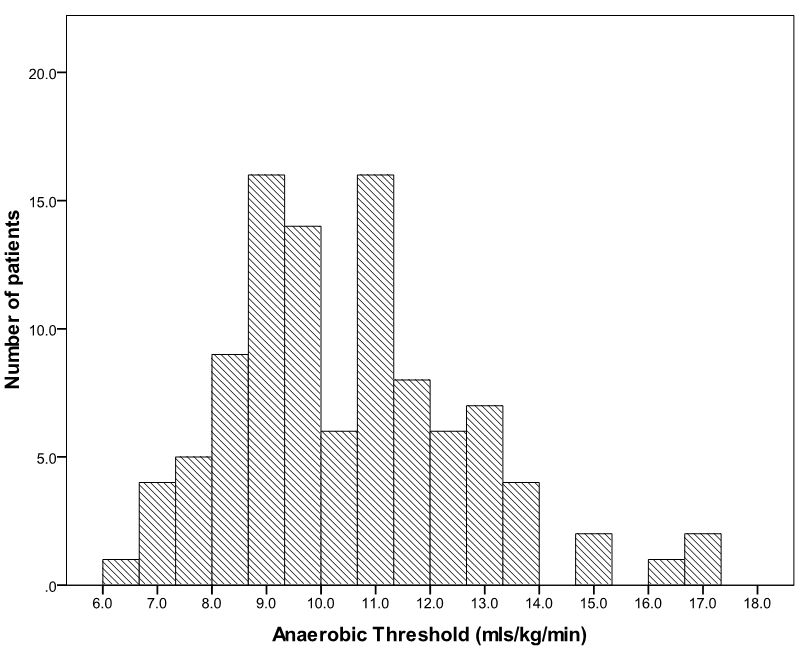
\includegraphics[width=0.8\linewidth]{Figures/cpet_outcomes_dist_of_AT}
	\caption{Distribution of $\dot{V}_{O_2}$AT across the study population.}
	\label{fig:cpet_outcomes_dist_of_AT}
\end{figure}

\subsection{Anaerobic threshold vs. complications}
The relationship between $\dot{V}_{O_2}$AT and major postoperative adverse events including mortality is shown in Table \ref{table:cpet_outcomes_table2}. 
Patients with $\dot{V}_{O_2}$AT less than 10 ml/kg/min had significantly greater incidence of postoperative pancreatic fistula (35.4\% vs.16\%, p=0.028) as well as major intra-abdominal abscesses (Clavien-Dindo Grade III - V, 22.4\% vs.7.8\%, p=0.042). 
While there was an association between low $\dot{V}_{O_2}$AT and grade of pancreatic fistula, this was not statistically significant (p=0.091). 
There was no association between low $\dot{V}_{O_2}$AT and cardiopulmonary complications or postoperative mortality. 
Major cardiopulmonary complications occurred more often in patients with major intra-abdominal adverse events including major intra-abdominal abscesses or Grade B and C pancreatic fistulae or haemorrhage than in patients who did not have these complications (5/31,16.1\% vs. 2/69,2.9\%, p=0.017). 
Postoperative mortality was not associated with $\dot{V}_{O_2}$AT (HR 0.77, 95\% CI 0.16-3.61, p 0.737) or the POSSUM Physiology Score (HR 0.39, 95\% CI 0.07-2.12, p 0.277). 
Postoperative mortality was associated with postoperative pancreatic fistula (n=5), post-pancreatectomy haemorrhage (n=3), major intra-abdominal sepsis (n=6) and major cardiorespiratory complications (n=4) with 6 patients requiring radiological or operative intervention.

%Table 2
\begin{table}[p]
	\centering
	\caption{The relationship between anaerobic threshold and complications in patients undergoing major pancreatic surgery.}
	\label{table:cpet_outcomes_table2}
	\renewcommand{\arraystretch}{1.2} %Increases space between rows
	\setlength{\tabcolsep}{12pt} %sets the space between columns

	
	\begin{tabular}{|C{1cm} l c c c c|}
		\hline
		\multicolumn{2}{|l}{Complications} &    & $\dot{V}_{O_2}$AT $\geq$10 & $\dot{V}_{O_2}$AT $<$ 10 &  \\
		 &                                 & n  & n                          & n                        & \textit{p} \\ \hline
		\multicolumn{6}{|l|}{Cardiac complications}                                                             \\
		 & Grade 0 - II                    & 99 & 51                         & 48                       & 0.308 \\
		 & Grade III - V                   & 1  & 0                          & 1                        &  \\
		\multicolumn{6}{|l|}{Respiratory complications}                                                         \\
		 & Grade 0 - II                    & 93 & 48                         & 45                       & 0.657 \\
		 & Grade III - V                   & 7  & 3                          & 4                        &  \\
		\multicolumn{6}{|l|}{Intra-abdominal abscess}                                                           \\
		 & Grade 0 - II                    & 85 & 47                         & 38                       & 0.042 \\
		 & Grade III - V                   & 15 & 4                          & 11                       &  \\
		\multicolumn{6}{|l|}{Pancreatic Fistula (Total/Sub-total pancreatectomies excluded)}                    \\
		 & No                              & 73 & 42                         & 31                       & 0.028 \\
		 & Yes                             & 25 & 8                          & 17                       &  \\
		\multicolumn{6}{|l|}{Pancreatic Fistula (ISGPS Classification)}                                         \\
		 & No                              & 73 & 42                         & 31                       & 0.091 \\
		 & Grade A                         & 9  & 3                          & 6                        &  \\
		 & Grade B                         & 8  & 1                          & 7                        &  \\
		 & Grade C                         & 8  & 4                          & 4                        &  \\
		\multicolumn{6}{|l|}{Post-Pancreatectomy Haemorrhage (ISGPS Classification)}                            \\
		 & No                              & 84 & 41                         & 43                       & 0.207 \\
		 & Grade A                         & 4  & 2                          & 2                        &  \\
		 & Grade B                         & 4  & 2                          & 2                        &  \\
		 & Grade C                         & 8  & 6                          & 2                        &  \\
		\multicolumn{6}{|l|}{Admissions to critical care}                                                       \\
		 & 1                               & 74 & 38                         & 36                       & 0.906 \\
		 & $>$1                            & 26 & 13                         & 13                       &  \\
		\multicolumn{6}{|l|}{Reoperation}                                                                       \\
		 & No                              & 89 & 47                         & 42                       & 0.306 \\
		 & Yes                             & 11 & 4                          & 7                        &  \\
		\multicolumn{6}{|l|}{Operative mortality}                                                               \\
		 & No                              & 93 & 47                         & 46                       & 0.737 \\
		 & Yes                             & 7  & 4                          & 3                        &  \\ \hline
		 \multicolumn{6}{l}{\textit{p} - Chi-square test}                                                               \\
	\end{tabular}
\end{table}

\subsection{Anaerobic threshold vs. length of stay}
The median length of postoperative stay was 17 days (IQR 13 - 26). 
The median cumulative length of stay in critical care was 7 days (IQR 6 - 12). 
Twenty-six patients were admitted to critical care more than once. 
The relationship between preoperative clinico-pathological characteristics and length of postoperative stay in patients who were discharged from hospital (n=93) is shown in Table \ref{table:cpet_outcomes_table3}. 
On univariate analysis, age over 65 years (p=0.072) and low $\dot{V}_{O_2}$AT (p=0.010) were associated with prolonged postoperative stay. 
On multivariate Cox proportional hazards regression analysis, $\dot{V}_{O_2}$AT less than 10 ml/kg/min (hazard ratio 1.74, 95\% confidence intervals 1.14-2.65, p=0.010) was the only significant factor associated with prolonged postoperative stay. 
A Kaplan-Meier plot for the probability of remaining in hospital over time for patients with low or normal $\dot{V}_{O_2}$AT is shown in Figure \ref{fig:cpet_outcomes_km_at_los}. 
Patients with a low $\dot{V}_{O_2}$AT stayed a median 6 days longer in hospital (14 versus 20 days, Mann-Whitney Test p=0.001). 
There was no significant association between any of the preoperative factors including $\dot{V}_{O_2}$AT and length of critical care stay or number of critical care admissions.

% Table 3
\begin{table}[p]
	\centering
	\caption{The relationship between clinico-pathological characteristics and postoperative stay in patients (excluding operative mortality) undergoing major pancreatic surgery (n=93): Cox regression analysis}
	\label{table:cpet_outcomes_table3}
	\renewcommand{\arraystretch}{1.2} %Increases space between rows
	\setlength{\tabcolsep}{9pt} %sets the space between columns

	\begin{tabular}{|C{1cm} l c c c c c c c|}
		\hline
		\multicolumn{2}{|l}{Variable} & n  & HR   & 95\% CI   & P     & HR   & 95\% CI   & p     \\ \hline
		\multicolumn{9}{|l|}{Age (years)}                                                       \\
		 & $\leq$ 65                 & 44 &      &           &       &      &           &  \\
		 & $>$ 65                    & 49 & 1.47 & 0.97-2.24 & 0.072 & 1.48 & 0.97-2.25 & 0.068 \\
		\multicolumn{9}{|l|}{Sex}                                                               \\
		 & Male                      & 56 &      &           &       &      &           &  \\
		 & Female                    & 37 & 1.32 & 0.86-2.03 & 0.199 &      &           &  \\
		\multicolumn{9}{|l|}{BMI (kg/sq.m)}                                                     \\
		 & $\leq$ 25                 & 42 &      &           &       &      &           &  \\
		 & $>$ 25                    & 51 & 0.87 & 0.58-1.32 & 0.512 &      &           &  \\
		\multicolumn{9}{|l|}{Smoking}                                                           \\
		 & No                        & 56 &      &           &       &      &           &  \\
		 & Yes                       & 37 & 1.26 & 0.82-1.94 & 0.294 &      &           &  \\
		\multicolumn{9}{|l|}{POSSUM Physiology Score}                                           \\
		 & $\leq$ 14                 & 45 &      &           &       &      &           &  \\
		 & $>$ 14                    & 48 & 1.28 & 0.85-1.95 & 0.24  &      &           &  \\
		\multicolumn{9}{|l|}{Preoperative Biliary Drainage}                                     \\
		 & No                        & 53 &      &           &       &      &           &  \\
		 & Yes                       & 40 & 1.08 & 0.71-1.65 & 0.724 &      &           &  \\
		\multicolumn{9}{|l|}{Serum Bilirubin (micromol/L)}                                      \\
		 & $\leq$  35                & 54 &      &           &       &      &           &  \\
		 & $>$  35                   & 39 & 1.26 & 0.83-1.92 & 0.277 &      &           &  \\
		\multicolumn{9}{|l|}{mGPS}                                                              \\
		 & 0                         & 59 &      &           &       &      &           &  \\
		 & 1                         & 5  & 1.22 & 0.78-1.92 & 0.387 &      &           &  \\
		 & 2                         & 29 & 1.87 & 0.71-4.88 & 0.204 &      &           &  \\
		\multicolumn{9}{|l|}{Haemoglobin (g/dl)}                                                \\
		 & $\geq$ 12                 & 57 &      &           &       &      &           &  \\
		 & $<$ 12                    & 36 & 1.19 & 0.78-1.81 & 0.422 &      &           &  \\
		\multicolumn{9}{|l|}{Anaerobic Threshold  (ml/kg/min)}                                  \\
		 & $\geq$ 10                 & 47 &      &           &       &      &           &  \\
		 & $<$ 10                    & 46 & 1.74 & 1.14-2.64 & 0.01  & 1.74 & 1.14-2.65 & 0.01  \\
		\multicolumn{9}{|l|}{Anaerobic Threshold (ml/kg/min)}                                   \\
		 & $\geq$ 11                 & 33 &      &           &       &      &           &  \\
		 & $<$ 11                    & 60 & 1.44 & 0.94-2.22 & 0.097 &      &           & 0.395 \\ \hline
	\end{tabular}
\end{table}

% Figure 2
\begin{figure}[h]
\centering
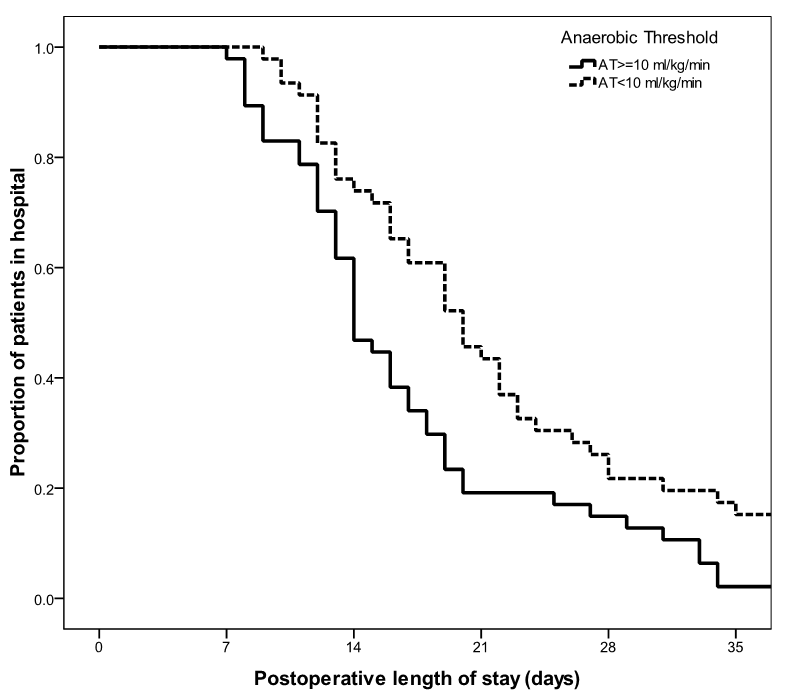
\includegraphics[width=0.8\linewidth]{Figures/cpet_outcomes_km_at_los}
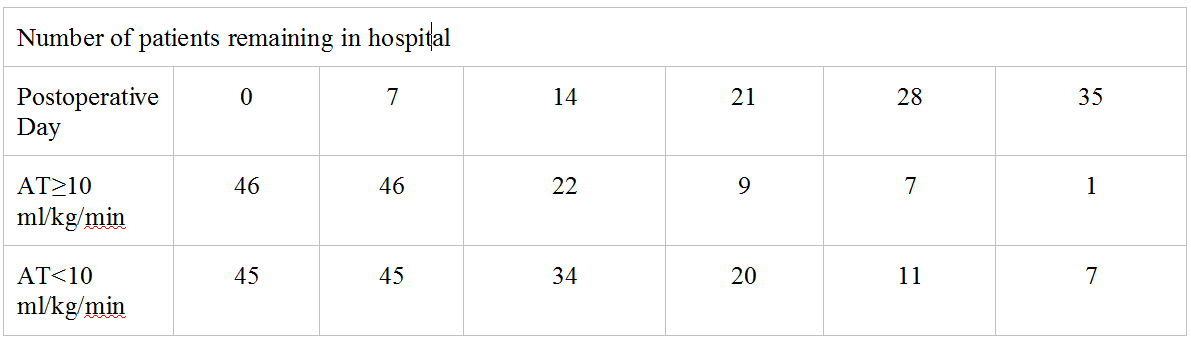
\includegraphics[width=1\linewidth]{Figures/cpet_outcomes_km_at_los_table} %Table below Kaplan Meier curve
\caption{Kaplan-Meier Plot of postoperative length of stay in patients with $\dot{V}_{O_2}$AT $>=$ 10 ml/kg/min versus $<$ 10 ml/kg/min.}
\label{fig:cpet_outcomes_km_at_los}
\end{figure}

\subsection{Anaerobic threshold vs. receipt of adjuvant therapy}
The relationship between clinico-pathological patient factors and receipt of adjuvant therapy is shown in Table \ref{table:cpet_outcomes_table4}. 
Fifty-five patients were included in the analysis. 
Patients were excluded if chemotherapy was not indicated (n=28), in the event of operative mortality (n=7), if chemotherapy was offered but declined by the patient (n=4), or where they had not been seen by an oncologist yet (n=6). 
On binary logistic regression analysis, $\dot{V}_{O_2}$AT less than 10 ml/kg/min was the only preoperative factor that was associated with with non-receipt of adjuvant therapy (HR 6.30, 95\% CI 1.25-31.75, p=0.026). 

%Table 4
\begin{table}[p]
	\caption{The relationship between clinico-pathological characteristics and receipt of adjuvant therapy in patients undergoing major pancreatic surgery (n = 55) - Binary logistic regression}
	\label{table:cpet_outcomes_table4}
	\centering
	\renewcommand{\arraystretch}{1.2} %Increases space between rows
	\setlength{\tabcolsep}{14pt} %sets the space between columns
	\begin{tabular}{|C{1cm} l c c c c|}
		\hline
		\multicolumn{2}{|l}{Variable} & n = 55 & HR   & 95\% CI    & \textit{p}    \\ \hline
		\multicolumn{6}{|l|}{Age (years)}                                  \\
		 & $\leq$ 65                  & 25     &      &            &  \\
		 & $>$ 65                     & 30     & 2.63 & 0.71-9.74  & 0.149 \\
		\multicolumn{6}{|l|}{Sex}                                          \\
		 & Male                       & 31     &      &            &  \\
		 & Female                     & 24     & 2.08 & 0.61-7.13  & 0.242 \\
		\multicolumn{6}{|l|}{BMI (kg/m$^2$)}                               \\
		 & $\leq$ 25                  & 25     &      &            &  \\
		 & $>$ 25                     & 30     & 0.78 & 0.23-2.64  & 0.693 \\
		\multicolumn{6}{|l|}{Smoking}                                      \\
		 & No                         & 35     &      &            &  \\
		 & Yes                        & 20     & 0.96 & 0.27-3.41  & 0.953 \\
		\multicolumn{6}{|l|}{POSSUM Physiology Score}                      \\
		 & $\leq$ 14                  & 25     &      &            &  \\
		 & $>$ 14                     & 30     & 1.63 & 0.46-5.73  & 0.447 \\
		\multicolumn{6}{|l|}{Preoperative Biliary Drainage}                \\
		 & No                         & 27     &      &            &  \\
		 & Yes                        & 28     & 0.95 & 0.28-3.21  & 0.937 \\
		\multicolumn{6}{|l|}{Serum Bilirubin ($\mu$mol/L)}                 \\
		 & $\leq$  35                 & 27     &      &            &  \\
		 & $>$  35                    & 28     & 2.08 & 0.60-7.30  & 0.251 \\
		\multicolumn{6}{|l|}{modified Glasgow Prognostic Score (mGPS)}     \\
		 & 0                          & 32     &      &            &  \\
		 & 1                          & 2      & 0    & 0          &  \\
		 & 2                          & 21     & 1.2  & 0.35-4.15  & 0.773 \\
		\multicolumn{6}{|l|}{Haemoglobin (g/dl)}                           \\
		 & $\geq$ 12                  & 31     &      &            &  \\
		 & $<$ 12                     & 24     & 0.96 & 0.28-3.26  & 0.946 \\
		\multicolumn{6}{|l|}{Anaerobic Threshold  (ml/kg/min)}             \\
		 & $\geq$ 10                  & 23     &      &            &  \\
		 & $<$ 10                     & 32     & 6.3  & 1.25-31.75 & 0.026 \\
		\multicolumn{6}{|l|}{Anaerobic Threshold  (ml/kg/min)}             \\
		 & $\geq$ 11                  & 16     &      &            &  \\
		 & $<$ 11                     & 39     & 3.11 & 0.61-15.88 & 0.172 \\ \hline
	\end{tabular}
	 %\todo{These AT numbers dont make sense. Why are there more patients with low AT? Check this.}
	 %These numbers are correct. Should I use simple chi-square test instead?
\end{table}

\clearpage

\section{Discussion}
The results of the present study show that a low $\dot{V}_{O_2}$AT is associated with prolonged postoperative stay in hospital, postoperative pancreatic fistula and intra-abdominal abscesses in patients undergoing major resections for pancreatic head lesions. 
The results of this study also show that patients with low $\dot{V}_{O_2}$AT are less likely to receive adjuvant therapy. 

Therefore, it would appear that objective measurement of patient physiological fitness using cardiopulmonary exercise testing is superior to conventional measures of patient fitness including the POSSUM Physiology Score or the modified Glasgow Prognostic Score and may have a role in predicting short-term outcome which in turn affects the overall management of these patients including receipt of adjuvant therapy.

Patients with a low $\dot{V}_{O_2}$AT stayed longer in hospital after their operation. 
While length of stay in hospital is influenced by multiple factors including postoperative complications, it would appear that patients with a low $\dot{V}_{O_2}$AT take longer to recover from the physiological stress placed by major pancreatic surgery and its sequelae.

The incidence of pancreatic fistula was greater in patients with a low $\dot{V}_{O_2}$AT. 
This association needs further evaluation taking into consideration other well-recognised risk factors for pancreatic fistula such as pancreatic texture, pancreatic duct size and intra-operative blood loss \parencite{braga_prognostic_2011, pratt_possum_2008, winter_1423_2006}. 
It is possible that local or operative factors may be compounded by poor oxygen delivery and organ perfusion as measured by cardiopulmonary exercise testing. 
There was a non-significant trend towards clinically relevant pancreatic fistulae (ISGPS Grades B and C) as well as a significant association with major intra-abdominal abscesses (Clavien-Dindo Grades 3-5 i.e., requiring intervention, associated with organ dysfunction requiring intensive care or resulting in mortality). 
This would suggest that complications in patients with low $\dot{V}_{O_2}$AT are more likely to be severe than in patients with normal $\dot{V}_{O_2}$AT. 
However, there was no difference in mortality between patients with normal or low $\dot{V}_{O_2}$AT, indicating that multiple factors including preoperative patient fitness, local and operative factors, systemic inflammatory response, number of complications as well as perioperative critical care all play a role.

The results of this study also show that patients with a low $\dot{V}_{O_2}$AT were less likely to receive adjuvant therapy. 
Adjuvant therapy in patients undergoing pancreatic resections for cancer has been shown in multiple randomised trials to improve survival significantly \parencite{neoptolemos_randomized_2004, neoptolemos_adjuvant_2009}
While postoperative mortality after pancreatic surgery has steadily improved over the years with major improvements in the quality of surgical and critical care over the past decade \parencite{winter_1423_2006} even in elderly patients \parencite{makary_pancreaticoduodenectomy_2006}, postoperative morbidity remains high \parencite{mann_review_2010}. 
The results of this study show that poor preoperative fitnees is not only associated with a protracted protracted postoperative course with complications but also with non-receipt of adjuvant therapy.

In the present study, $\dot{V}_{O_2}$AT was less than 10 ml/kg/min in 49\% of patients and less than 11 ml/kg/min in 64\% of patients. 
The proportion of patients with $\dot{V}_{O_2}$AT less than 11 ml/kg/min in this study was much greater than reported in studies involving patients undergoing oesophageal surgery (16\%),\parencite{forshaw_is_2008} liver transplantation (39\%)\parencite{epstein_aerobic_2004} or other major abdominal surgery (29\%)\parencite{older_preoperative_1993} and may indicate the poor preoperative fitness levels of patients undergoing major pancreatic surgery at our unit. 
While several studies have shown that low $\dot{V}_{O_2}$AT and/or low $\dot{V}_{O_2}$peak are associated with postoperative complications or prolonged hospital stay following major abdominal surgery as well as non-abdominal surgery,\parencite{older_preoperative_1993, epstein_aerobic_2004, mccullough_cardiorespiratory_2006, nagamatsu_preoperative_2001, older_cardiopulmonary_1999, older_clinical_2004} others have disputed this \parencite{forshaw_is_2008, clayton_cardiopulmonary_2011, hightower_pilot_2010}. 
Older and co-workers reported in 1993 that low $\dot{V}_{O_2}$AT less than 11 ml/kg/min was associated with a significantly higher risk of postoperative mortality from cardiovascular causes in a series of 187 elderly patients undergoing major abdominal surgery \parencite{older_preoperative_1993}.

However, Snowden and co-workers \parencite{snowden_submaximal_2010} reported that patients with an $\dot{V}_{O_2}$AT less than 10.1 ml/kg/min had significantly greater cardiopulmonary complications as well as non-cardiopulmonary and infectious complications while Forshaw and co-workers \parencite{forshaw_is_2008} reported that using a cut-off of 11 ml/kg/min for the $\dot{V}_{O_2}$AT did not predict postoperative adverse events less after oesophagectomy. 
The lack of association between low $\dot{V}_{O_2}$AT and cardiopulmonary complications in this study may have been due to two reasons. 
Major cardiopulmonary complications occurred more often in association with major intra-abdominal adverse events which are determined largely by pancreatic morphology and local anatomy \parencite{braga_prognostic_2011}. 
Moreover, the stringent fitness criteria for undergoing pancreaticoduodenectomy may have excluded patients with known co-morbid cardiorespiratory diseases such as severe chronic obstructive pulmonary disease or cardiac failure.

The results of this study are consistent with the findings by Ausania and co-workers \parencite{ausania_effects_2012} who reported increased incidence of pancreatic fistula and prolonged postoperative stay in patients with $\dot{V}_{O_2}$AT less than 10.1 ml/kg/min. 
However, this study did not report the association between $\dot{V}_{O_2}$AT and receipt of adjuvant therapy.

The physiological demands placed on a patient undergoing major pancreatic surgery are significant, both during and after the operation. 
It is not entirely surprising therefore, that conventional parameters of patient fitness like the POSSUM Physiology Score or the modified Glasgow Prognostic Score are limited in their ability to distinguish patients based on their performance under physiological stress. 
Cardiopulmonary exercise testing overcomes this disadvantage by replicating some of the physiological burden major pancreatic surgery places on the functional capacity of the patient's cardiovascular and respiratory systems.

This functional capacity of patients to withstand the physiological burden of major surgery can be improved by the process of `prehabilitation' \parencite{topp_effect_2002}. 
It has been suggested that prehabilitation not only improves aerobic capacity \parencite{jones_effects_2007} but may also improve postoperative recovery \parencite{mayo_impact_2011, pehlivan_effects_2011}. 
The results of this study show that impaired aerobic capacity is associated with postoperative adverse events. 
Therefore, it would appear that prehabilitation using interventions such as exercise and nutrition, by improving physiological fitness, may have a role in improving postoperative outcomes after major pancreatic surgery and may improve the proportion of patients receiving adjuvant therapy.

Further work needs to be carried out to study the value of cardiopulmonary exercise testing in predicting postoperative complications in conjunction with previously established factors such as pancreatic morphology and operative factors before it can be used on its own to select or exclude patients for pancreaticoduodenectomy. 
Cardiopulmonary exercise testing would play an important role not only in identifying patients who will benefit from prehabilitation, but also in the objective measurement of the effects of such interventions on aerobic capacity as well as in identifying high risk patients who may not be able to complete oncological treatment. 
Prehabilitation and optimised perioperative care may allow a greater proportion of high risk patients to progress to oncological treatment after surgery. 
%%CPET and Jaundice

\chapter{An investigation into the relationship between cardiopulmonary exercise testing, preoperative pathophysiology and obstructive jaundice in patients undergoing pancreaticoduodenectomy.}

\label{ch_cpet_jaundice}
\lhead{Chapter \ref{ch_cpet_jaundice}. \emph{CPET, Jaundice and Preoperative Pathophysiology}}
\clearpage

%----------------------------------------------------------------------------------------

\section{Introduction}
Patients with tumours involving the pancreatic head or the periampullary region often present with inoperable disease. 
In the minority of patients with operable disease, resectional surgery in the form of a pancreaticoduodenectomy remains the main modality of treatment and only chance of a potential cure. 
However, major pancreatic surgery is associated with significant morbidity and mortality and is only undertaken in specialist centres. 
Patient selection, preoperative optimisation, good surgical technique and improvements in postoperative care have all contributed to a reduction in mortality \parencite{winter_1423_2006} but morbidity remains high \parencite{mann_review_2010}.
While several technical strategies have been described in recent years to minimise morbidity, these strategies are not necessarily based on a better understanding of the physiological basis of postoperative complications in these patients.

The close anatomical relationship between the distal bile duct, distal pancreatic duct, head of the pancreas and the duodenum is responsible for obstructive jaundice being the most common presenting symptom in patients with tumours affecting this region. 
Distal bile duct strictures also occur in a proportion of patients with severe chronic pancreatitis involving the pancreatic head.
In such patients, it may be impossible to distinguish inflammation from malignant disease on preoperative imaging and a proportion of these patients will require a pancreaticoduodenectomy \parencite{abraham_pancreaticoduodenectomy_2003}.
The perioperative management of the patient with obstructive jaundice is complex and management algorithms are still evolving \parencite{wang_preoperative_2008}. 

Obstructive jaundice has been shown to be associated with abnormal cardiovascular physiology in several animal and human studies. 
Surgery in the jaundiced patient has been reported to be associated with adverse postoperative haemodynamic events and renal dysfunction \parencite{pain_perioperative_1985,green_systemic_1995}. 
The association between jaundice and cardiovascular physiology was reported over a hundred years ago by King and co-workers who found that injection of porcine bile pigment into dogs resulted in bradycardia, hypotension and eventually death \parencite{king_effect_1909}. 
Green and co-workers (1986) described the effects of `cholemia' in dogs that were subjected to choledochocaval anastomosis. 
The resultant myocardial depression was described by them as the `jaundiced heart' \parencite{green_jaundiced_1986} and was associated with poor myocardial response to inotropic stimulation in dogs \parencite{binah_obstructive_1985, bomzon_systemic_1986} as well as humans \parencite{lumlertgul_jaundiced_1991}.

As a result, preoperative biliary drainage (PBD) used to be advocated routinely before subjecting a patient to pancreaticoduodenectomy with the intention of reducing postoperative morbidity. 
A recent multi-center, randomised trial found that PBD was associated with increased incidence of complications after pancreaticoduodenectomy \parencite{van_der_gaag_preoperative_2010}.
However, this trial excluded patients with a bilirubin levels greater than 250 $\mu$mol/l from the study. 
A Cochrane meta-analysis of 6 studies including 520 patients also concluded that pre-operative biliary drainage was associated with increased incidence of complications and should not be used routinely in patients scheduled to undergo pancreaticoduodenectomy \parencite{fang_pre-operative_2012}.

\subsection{Aim}
The results presented in Chapter \ref{ch_cpet_outcomes} demonstrated that poor performance at cardiopulmonary exercise testing (CPET) was associated with adverse outcomes after pancreaticoduodenectomy with an increased incidence of POPF and prolonged hospital stay. 
Obstructive jaundice was present in a large proportion of these patients but not associated with prolonged hospitalisation (Table \ref{table:cpet_outcomes_table3}).
The aim of the present study was to evaluate the relationship between cardiopulmonary exercise testing, obstructive jaundice (especially severe obstructive jaundice with serum bilirubin $>$ 250 $\mu$mol/l) and preoperative pathophysiology in patients undergoing pancreaticoduodenectomy.

\clearpage

\section{Patients and methods}

\subsection{Patients}
Patients who underwent classical or pylorus-preserving pancreaticoduodenectomy for periampullary lesions (both benign and malignant) between August 2008 and December 2012 and had undergone cardiopulmonary exercise testing as part of their preoperative assessment at the West of Scotland Pancreatic Unit, Glasgow Royal Infirmary, Glasgow were included in the study. 
Established criteria for resectability in patients with malignant disease were used as outlined in Section \ref{sec:resectability_criteria}. 
Segmental or wedge resection of the portal vein or superior mesenteric vein was carried out if the lesion was otherwise resectable.

\subsection{Preoperative data}
Patient demographics, preoperative clinico-pathological characteristics including cardiorespiratory comorbidity, results of preoperative blood tests, chest x-ray, ECG and cardiopulmonary exercise tests were collected from prospectively held databases. 
The POSSUM Physiology Score was calculated based on 11 physiological parameters (cardiac disease, respiratory disease, ECG changes, pulse rate, blood pressure, haemoglobin, white cell count, serum sodium, serum potassium, serum urea and Glasgow Coma Scale) and was used as an objective score of comorbidity (Table \ref{table:intro_possum} on p\pageref{table:intro_possum}).
Cardiovascular comorbidity was defined as a score of 2 or more for either the cardiac disease or ECG component of the POSSUM score. 
Respiratory comorbidity was defined as a score or 2 or more for the respiratory disease component of the POSSUM score. 

\subsection{Obstructive jaundice}
Serum bilirubin levels and liver function tests were measured in all patients on the day before surgery. 
Obstructive jaundice was defined as serum bilirubin $>$ 35 $\mu$mol/litre and severe obstructive jaundice was defined as serum bilirubin $>$ 250 $\mu$mol/litre. 
These thresholds were chosen as a recent randomised controlled trial that demonstrated increased complications in patients who underwent PBD excluded patients with serum bilirubin $>$ 250 $\mu$mol/litre from the study \parencite{van_der_gaag_preoperative_2010}.
The present study aimed to evaluate preoperative pathophysiology in this particular group of patients with `severe obstructive jaundice'.
Due to referral practices at the time of this study, a proportion of patients underwent preoperative biliary interventions and drainage before referral to the West of Scotland Pancreatic Unit. 
Data regarding biliary intervention and stenting was collected where feasible.

\subsection{Cardiopulmonary exercise test}
Cardiopulmonary exercise tests were performed in the Department of Respiratory Medicine at the Glasgow Royal Infirmary using the ZAN-600 CPET suite (nSpire Health, Longmont, CO 80501, USA). 
All patients underwent standard pulmonary function tests and spirometry prior to cardiopulmonary exercise testing. 
A cycle ergometer was used to perform a symptom-limited, incremental work-load test preceded by a 3-minute rest period. 
The test was stopped when patients achieved their maximum exercise tolerance, when significant ischaemic changes occurred on ECG or for other safety reasons. 
Peak oxygen consumption achieved at this stage was defined as $\dot{V}_{O_2}$Peak. 
The $\dot{V}_{O_2}$AT was calculated using the V-slope \parencite{beaver_new_1986,sue_metabolic_1988} and ventilatory equivalents \parencite{society_ats/accp_2003} methods.
$\dot{V}_{O_2}$AT less than 10 ml/kg/min was considered to be low based on previous work by us (Chapter \ref{ch_cpet_outcomes}) as well as Ausania and co-workers \parencite{ausania_effects_2012} which has shown increased incidence of complications in patients with $\dot{V}_{O_2}$AT below this threshold. 
Oxygen consumption at peak exercise ($\dot{V}_{O_2}$Peak) was dichotomised using a cut-off of 16 ml/kg/min. 
Cardiopulmonary exercise testing methodology and calculation of $\dot{V}_{O_2}$AT is described in detail in Sections \ref{sec:cpx_method} and \ref{sec:cpx_at_method}.
The cardiopulmonary exercise testing parameters described in this study are explained in detail in Section \ref{sec:cpx_parameters} on p\pageref{sec:cpx_parameters} and in published literature \parencite{balady_clinicians_2010}.

\subsection{Statistics}
Grouping of the variables was carried out using standard or previously published thresholds. 
In the absence of such thresholds, the variables were treated as continuous variables. 
Non-parametric tests were used to analyse the association between categorical and continuous variables while Chi-square tests were used to analyse the association between categorical variables. 
Univariate and multivariate binary logistic regression analysis was used to study the relationship between preoperative patient characteristics and $\dot{V}_{O_2}$AT / $\dot{V}_{O_2}$Peak. 
Scatter-plots were used for visual representation of the relationship between serum bilirubin and $\dot{V}_{O_2}$.

The level of significance was set at $p<0.05$.
SPSS software (Version 17.0; SPSS Inc., Chicago, IL, USA) was used to perform statistical analysis.

\clearpage

\section{Results}

\subsection{Clinico-pathological characteristics}
One-hundred and thirty eight patients underwent pancreaticoduodenectomy with preoperative cardiopulmonary exercise testing during the study period. 
Over half of the patients were male (n=93, 67\%). 
Approximately half the number of patients were over the age of 65 (n=68, 49\%) and overweight or obese (n=69, 50\%). 
Cardiovascular comorbidity was present in 58 patients (42\%) and respiratory comorbidity was present in 12 patients (9\%). 
Fifty patients (36\%) had a history of cigarette smoking. 
The POSSUM Physiology Score was greater than 14 in 61 patients (44\%). 
Obstructive jaundice (serum bilirubin 35-250 $\mu$mol/l) was present in 32 (23\%) patients while severe obstructive jaundice (serum bilirubin $>$ 250 $\mu$mol/l) was present in 19 (14\%) patients. 

The baseline demographic and clinical characteristics of non-jaundiced and jaundiced patients are shown in Table \ref{table:cpet_oj_patient}. 
A greater proportion of jaundiced patients were females (p=0.028) and smokers (p=0.038) compared to the non-jaundiced cohort. 
Elevated POSSUM Physiology Score (p=0.004) and malignancy (p$<$0.001) were significantly associated with the presence of jaundice. 
However, there was no statistically significant difference in age, body mass index, cardiovascular comorbidity, respiratory comorbidity or PBD between the non-jaundiced and jaundiced patients.

%OJ - PREOP CHARACTERISTICS
\begin{table}[p]
\caption{The relationship  between obstructive jaundice and preoperative patient characteristics in patients undergoing pancreaticoduodenectomy.}
\label{table:cpet_oj_patient}
\centering\renewcommand{\arraystretch}{1.4} %Increases space between rows
\setlength{\tabcolsep}{10pt} %sets the space between columns
	\begin{tabular}{| l | c c c c c |}
		\hline
		                             & \multicolumn{5}{c|}{Preoperative Serum Bilirubin ($\mu$mol/L)} \\
		n = 138                      & $\leq$ 17 & 18-35 & 35-250 & $>$ 250 & \textit{p}              \\ \hline
		Age ($\leq$65/$>$65 years)   & 32/33     & 13/9  & 16/16  & 9/10    & 0.935                   \\
		Sex (Male/Female)            & 48/17     & 14/8  & 22/10  & 9/10    & 0.028                   \\
		BMI (Normal/Overweight)      & 30/35     & 12/10 & 20/12  & 7/12    & 0.82                    \\
		Smoking (No / Yes)           & 48/17     & 12/10 & 18/14  & 10/9    & 0.038                   \\
		PPS ($\leq$14/$>$14)         & 39/22     & 16/5  & 9/23   & 8/11    & 0.004                   \\
		Cardiac disease (No/Yes)     & 35/28     & 13/9  & 17/15  & 13/6    & 0.539                   \\
		Respiratory disease (No/Yes) & 57/6      & 20/2  & 29/3   & 18/1    & 0.664                   \\
		Biliary Stent (No/Yes)       & 29/20     & 3/12  & 6/17   & 18/0    & 0.201                   \\
		Cancer (No/Yes)              & 26/39     & 3/19  & 3/29   & 0/19    & $<$0.001                \\ \hline
		\multicolumn{6}{l}{\textit{p} - Chi-square test}
	\end{tabular}
	\medskip
	\caption*{Obstructive jaundice was more common in females, smokers, patients with elevated POSSUM Physiology Score (PPS) and in patients with cancer. BMI - Body Mass Index, PPS - POSSUM Physiology Score}
\end{table}

\subsection{Obstructive jaundice vs. preoperative blood tests}
The relationship between obstructive jaundice and preoperative blood tests is shown in Table \ref{table:cpet_oj_bloods}. 
Obstructive jaundice was associated with the presence of a systemic inflammatory response as characterised by raised serum C-reactive protein levels and decrease in serum albumin levels (p$<$0.001). 
The degree of systemic inflammation was proportionate to the severity of jaundice. 
Non-jaundiced patients had a median CRP of 3.6 mg/l (inter-quartile range 0.3 - 89) and serum albumin of 37 g/l (IQR 18 - 46) while patients with severe obstructive jaundice had a median CRP of 13 (IQR 1.7 - 51) and a median serum albumin of 25 g/l (IQR 18 - 33). 
Obstructive jaundice was also associated with electrolyte abnormalities including serum sodium, serum potassium and serum chloride levels. 
Jaundiced patients were more likely to be anaemic (p$<$0.001) with lower haematocrit (p$<$0.001) and lower mean corpuscular volume (p=0.001). 
However, there was no significant difference in the preoperative renal function, prothrombin time and white cell count between jaundiced and non-jaundiced patients. 

%Table 2
	\begin{sidewaystable}[p]
		\caption{The relationship  between obstructive jaundice and preoperative biochemical parameters in patients undergoing pancreaticoduodenectomy. }
		\label{table:cpet_oj_bloods}
		\centering
		\renewcommand{\arraystretch}{1.4} %Increases space between rows
		\setlength{\tabcolsep}{9pt} %sets the space between columns
		
		\begin{tabular}{| l | c c c c c|}
			\hline
			                           &                   \multicolumn{4}{c}{Preoperative Serum Bilirubin}  &                 \\
			                           & $\leq$ 17        & 18-35            & 35-250           & $>$ 250          & \textit{p}       \\ \hline
			Haemoglobin                & 13.0 (12.1-14.1) & 13.2 (12.5-14.2) & 11.9 (11.1-12.4) & 11.7 (11.3-12.5) & $<$0.001 \\
			Haematocrit                & 0.39 (0.37-0.42) & 0.4 (0.38-0.43)  & 0.35 (0.34-0.37) & 0.36 (0.34-0.37) & $<$0.001 \\
			Mean Corpuscular Volume    & 90.1 (86.8-93.7) & 93.9 (91.1-96.7) & 92.9 (87.9-96.7) & 87.9 (83.5-91.3) & 0.001    \\
			White cell count           & 7.6 (6.5-9.2)    & 7.6 (6.4-9.5)    & 8.2 (6.7-9.4)    & 7.0 (6.2-9.2)    & 0.591    \\
			Prothrombin time           & 11 (10-12)       & 11 (11-12)       & 11 (11-12)       & 11 (11-12)       & 0.618    \\
			Serum Urea                 & 5.0 (4.3-6.1)    & 5.2 (4.0-5.6)    & 5.5 (4.5-6.6)    & 4.5 (2.3-5.3)    & 0.093    \\
			Serum Creatinine           & 71 (64-80)       & 75 (62-94)       & 71 (62-80)       & 65 (53-72)       & 0.221    \\
			Serum Sodium               & 138 (136-140)    & 138 (136-139)    & 138 (135-140)    & 135 (130-137)    & 0.001    \\
			Serum Potassium            & 4.1 (3.9-4.5)    & 4.3 (4.1-4.5)    & 4.1 (3.75-4.25)  & 3.8 (3.6-4)      & $<$0.001 \\
			Serum Chloride             & 104 (102-106)    & 104 (101-106)    & 104 (99.5-106)   & 99 (93-103)      & 0.002    \\
			Aspartate transaminase     & 21 (17-30)       & 29 (27-48)       & 68.5 (33-144)    & 92.5 (70-116)    & $<$0.001 \\
			Alanine transaminase       & 25 (16-41)       & 31 (24-73)       & 86.5 (50-157.5)  & 95 (53-149)      & $<$0.001 \\
			Gamma-glutamyl transferase & 81 (35-267)      & 111 (56-402)     & 263 (107-947)    & 495 (150-951)    & $<$0.001 \\
			Alkaline phosphatase       & 110 (80-149)     & 150 (115-292)    & 233 (174-698.5)  & 372 (272-551)    & $<$0.001 \\
			C-reactive protein         & 3.6 (1.8-9.5)    & 4.3 (2.4-8)      & 6.9 (3.6-33.5)   & 13 (8.3-20)      & $<$0.001 \\
			Albumin                    & 37 (34-39)       & 36 (33-38)       & 31 (28-33)       & 25 (23-28)       & $<$0.001 \\ \hline
			\multicolumn{6}{l}{Values are median (inter-quartile range); \textit{p} - Kruskal-Wallis test}
		\end{tabular}
	\end{sidewaystable}
	
	

\subsection{Obstructive jaundice vs. pulmonary function tests}
Pulmonary function tests including forced vital capacity (FVC), forced expiratory volume in one second (FEV1) and their derived parameters (predicted FEV1, FEV1/FVC, predicted FEV1/FVC) were compared between jaundiced and non-jaundiced patients. 
There was a trend towards lower forced vital capacity with increasing severity of jaundice but this did not reach statistical significance (p=0.092). 
There was no association between the other pulmonary function tests and jaundice (Table \ref{table:cpet_oj_pft}).

%OJ - PFT
\begin{sidewaystable}[p]
	\caption{The relationship  between obstructive jaundice and pulmonary function tests in patients undergoing pancreaticoduodenectomy.}
	\label{table:cpet_oj_pft}
	\centering
	\renewcommand{\arraystretch}{1.4} %Increases space between rows
	\setlength{\tabcolsep}{9pt} %sets the space between columns
	
	\begin{tabular}{|l| c c c c|c|}
		\hline
		                    &              \multicolumn{4}{c|}{Preoperative Serum Bilirubin}              &  \\
		                    & $\leq$ 17        & 18-35            & 35-250            & $>$ 250          & \textit{p} \\ \hline
		FVC                 & 4.09 (3.49-4.69) & 3.76 (3.38-4.59) & 3.76 (3.16-4.05)  & 3.35 (2.85-4.38) & 0.092      \\
		FEV1                & 2.95 (2.39-3.51) & 2.90 (2.12-3.34) & 2.68 (2.37-3.07)  & 2.72 (2.2-3.28)  & 0.556      \\
		PREDICTED FEV1 (\%) & 105.0 (91-116)   & 98.50 (87-114)   & 103.0 (95-111.5)  & 101.0 (94-116)   & 0.761      \\
		FEV1/FVC            & 72.0 (65-77)     & 73.0 (65-78)     & 75.50 (70.5-79.5) & 78.0 (70-82)     & 0.115      \\
		PREDICTED FEV1/FVC  & 94.0 (87-102)    & 96.0 (86-100)    & 99.0 (93-103)     & 102.0 (88-108)   & 0.107      \\ \hline
		\multicolumn{6}{l}{Values are median (inter-quartile range); \textit{p} - Kruskal-Wallis test}
	\end{tabular}
\end{sidewaystable}





\subsection{Obstructive jaundice vs. CPET}
Cardiopulmonary exercise test parameters measured at the anaerobic threshold and at peak exercise were compared between jaundiced and non-jaundiced patients using the Kruskal-Wallis test. 
Obstructive jaundice was associated with lower tidal volume (p=0.017), lower absolute $\dot{V}_{O_2}$ (p=0.003), lower corrected $\dot{V}_{O_2}$ (p=0.029), lower oxygen pulse (p=0.037) and lower respiratory rate (p=0.022) at the anaerobic threshold.
At peak exercise, jaundice was associated with lower tidal volume (p=0.028), lower absolute $\dot{V}_{O_2}$Peak (p=0.007), lower absolute $\dot{V}_{CO_2}$ (p=0.016) and lower end-tidal $O_2$ or $PET_{O_2}$ (p=0.026). 
However, as shown in Tables \ref{table:cpet_oj_anaerobic} and \ref{table:cpet_oj_peak}, several of these associations were not linear with a trend towards poorer results between non-jaundiced and mildly jaundiced patients and better values in the severely jaundiced cohort. 

%OJ - ANAEROBIC THRESHOLD
\begin{sidewaystable}[p]
	\caption{The relationship  between obstructive jaundice and cardiopulmonary exercise test parameters at the anaerobic threshold in patients undergoing pancreaticoduodenectomy.  }
	\label{table:cpet_oj_anaerobic}
	\centering
	\renewcommand{\arraystretch}{1.2} %Increases space between rows
	%\setlength{\tabcolsep}{9pt} %sets the space between columns
		%6 columns   
	\begin{tabular}{|l| c c c c c|}
		\hline
		                               &             \multicolumn{4}{c}{Preoperative Serum Bilirubin ($\mu$mol/L)}             &  \\
		Anaerobic Threshold            & $\leq$ 17           & 18-35               & 35-250              & $>$ 250             & \textit{p} \\ \hline
		Load  (Watts)                  & 44.3 (32.5-60.0)    & 33.5 (27.5-51.0)    & 41.0 (31.0-56.0)    & 38.3 (30.5-48.0)    & 0.313      \\
		Min. Ventilation (l/min)       & 25.0 (20.4-30.5)    & 23.0 (20.5-29.0)    & 23.0 (19.0-28.0)    & 22.0 (18.5-25.0)    & 0.107      \\
		Tidal Volume (litres)          & 1.26 (1.06-1.52)    & 1.09 (0.83-1.39)    & 1.06 (0.94-1.44)    & 1.08 (0.82-1.26)    & 0.017      \\
		$\dot{V}_{O_2}$ (litres/min)   & 0.85 (0.71-1.00)    & 0.73 (0.62-0.81)    & 0.72 (0.58-0.86)    & 0.70 (0.58-0.82)    & 0.003      \\
		$\dot{V}_{O_2}$/kg (ml/kg/min) & 11.1 (9.8-12.8)     & 10.6 (8.9-11.4)     & 9.9 (8.5-12.7)      & 9.6 (9.3-10.8)      & 0.029      \\
		$\dot{V}_E/\dot{V}_{O_2}$      & 28.5 (25.5-30.1)    & 29.4 (26.7-31.3)    & 28.3 (27.0-34.7)    & 27.8 (24.6-31.9)    & 0.510      \\
		$\dot{V}_{CO_2}$ (litres/min)  & 0.82 (0.66-1.0)     & 0.71 (0.58-0.93)    & 0.75 (0.58-0.90)    & 0.69 (0.52-0.79)    & 0.032      \\
		$\dot{V}_E/\dot{V}_{CO_2}$     & 28.9 (27.2-30.7)    & 28.9 (28.1-30.7)    & 30.6 (26.3-33.1)    & 30.4 (27.9-32.2)    & 0.449      \\
		RER                            & 0.96 (0.9-1.03)     & 0.99 (0.89-1.04)    & 0.98 (0.94-1.07)    & 0.93 (0.91-1.04)    & 0.478      \\
		${PET_O}_2$ (mmHg)             & 110.0 (104.3-112.6) & 113.0 (109.0-115.0) & 111.0 (106.0-117.0) & 111.0 (105.0-114.5) & 0.078      \\
		${PET_{CO}}_2$ (mmHg)          & 36.8 (34.8-39.0)    & 36.0 (34.0-37.5)    & 34.0 (32.0-39.0)    & 35.0 (32.0-39.0)    & 0.204      \\
		$O_2$Pulse (ml/beat)           & 8.0 (7.0-9.0)       & 7.0 (5.0-9.0)       & 7.5 (5.0-9.0)       & 6.7 (5.0-8.0)       & 0.037      \\
		Heart rate (/min)              & 108 (96-122)        & 107 (90-118)        & 101 (89-118)        & 112 (96-125)        & 0.393      \\
		Respiratory Rate (/min)        & 19 (17-21)          & 22 (20-27)          & 21 (18-24)          & 19 (18-23)          & 0.022      \\ \hline
		\multicolumn{6}{l}{Values are median (inter-quartile range); \textit{p} - Kruskal-Wallis test}
	\end{tabular}
	\medskip
	\caption*{At anaerobic threshold, obstructive jaundice was compared to multiple CPET parameters. There were several statistically significant but non-linear relationships between preoperative serum bilirubin and CPET parameters. $\dot{V}_{O_2}$ - Oxygen consumption, $\dot{V}_{CO_2}$ - Exhaled $CO_2$, PET$O_2$/$CO_2$ - Partial pressure of end-tidal $O_2$/$CO_2$, $O_2$Pulse - Oxygen pulse.}
\end{sidewaystable}



%OJ - PEAK EXERCISE
\begin{sidewaystable}[p]
	\caption{The relationship  between obstructive jaundice and cardiopulmonary exercise test parameters at peak exercise in patients undergoing pancreaticoduodenectomy.  }
	\label{table:cpet_oj_peak}
	\centering
	\renewcommand{\arraystretch}{1.4} %Increases space between rows
	%\setlength{\tabcolsep}{9pt} %sets the space between columns
		%6 columns   
	\begin{tabular}{|l| c c c c c|}
		\hline
		                               &               \multicolumn{4}{c}{Preoperative Serum Bilirubin}                &  \\
		Peak Exercise                               & $\leq$ 17         & 18-35             & 35-250            & $>$ 250            & \textit{p} \\ \hline
		Load  (Watts)                  & 94.0 (76.5-114.5) & 87.5 (56.0-107.0) & 73.0 (58.0-108.0) & 85.0 (66.0-101.0)  & 0.066      \\
		Min. Ventilation (l/min)       & 53.5 (46.0-69.0)  & 46.5 (34.0-62.0)  & 46.0 (38.0-63.0)  & 48.0 (37.0-67.0)   & 0.088      \\
		Tidal Volume (litres)          & 1.95 (1.6-2.41)   & 1.64 (1.46-1.98)  & 1.62 (1.35-2.19)  & 1.86 (1.18-2.21)   & 0.028      \\
		$\dot{V}_{O_2}$ (litres/min)   & 1.33 (1.09-1.57)  & 1.14 (0.90-1.32)  & 1.08 (0.85-1.5)   & 1.11 (0.89-1.38)   & 0.007      \\
		$\dot{V}_{O_2}$/kg (ml/kg/min) & 17.2 (14.45-22.0) & 14.7 (13.5-17.3)  & 15.1 (12.7-19.9)  & 15.7 (13.3-19.2)   & 0.056      \\
		$\dot{V}_E/\dot{V}_{O_2}$      & 40.5 (36.2-46.8)  & 43.1 (37.3-46.5)  & 41.9 (38.9-47.4)  & 46.7 (42.1-55.2)   & 0.073      \\
		$\dot{V}_{CO_2}$ (litres/min)  & 1.67 (1.37-2.01)  & 1.32 (1.02-1.84)  & 1.29 (1.04-1.88)  & 1.47 (1.03-1.76)   & 0.016      \\
		$\dot{V}_E/\dot{V}_{CO_2}$     & 31.9 (29.5-34.9)  & 32.1 (29.4-36.4)  & 33.1 (30.2-37.8)  & 37.4 (30.9-40.8)   & 0.110      \\
		RER                            & 1.28 (1.20-1.42)  & 1.27 (1.20-1.42)  & 1.28 (1.22-1.36)  & 1.36 (1.25-1.42)   & 0.675      \\
		${PET_O}_2$                    & 121 (118.5-125)   & 122 (120-126)     & 122 (120-125)     & 126 (123-128)      & 0.026      \\
		${PET_{CO}}_2$                 & 35 (32.5-38)      & 35 (32-38)        & 34 (30-38)        & 33 (29-36)         & 0.283      \\
		$O_2$Pulse                     & 11.9 (9.11-14)    & 10.0 (8.0-12.0)   & 11.0 (9.61-13.93) & 11.65 (8.26-13.94) & 0.132      \\
		Heart rate                     & 140 (125-158)     & 140 (129-152)     & 129 (114-144)     & 134 (128-158)      & 0.158      \\
		Respiratory Rate               & 30 (26-34)        & 32 (28-35)        & 30 (26-34)        & 31 (28-36)         & 0.512      \\
		Exercise Duration (minutes)    & 8.2 (6.2-10.4)    & 6.9 (5.5-9.2)     & 6.6 (4.8-9.0)     & 8.2 (5.2-9.7)      & 0.164      \\ \hline
		\multicolumn{6}{l}{Values are median (inter-quartile range); \textit{p} - Kruskal-Wallis test}
	\end{tabular}
\end{sidewaystable}


Scatter-plot analysis comparing serum bilirubin versus $\dot{V}_{O_2}$AT and $\dot{V}_{O_2}$Peak as continuous variables is depicted in Figure \ref{fig:cpet_oj_scatter}. 
This shows that the relationship between serum bilirubin and $\dot{V}_{O_2}$AT is weak with a $\rho^2$ value of 0.035 Pearson's $\rho$ = - 0.187, p = 0.028. 
There was no correlation between serum bilirubin and $\dot{V}_{O_2}$Peak (Pearson's $\rho$ = - 0.132, $\rho^2$ = 0.017, p = 0.123)

\begin{figure}[htbp]
	\centering
	\begin{subfigure}{0.48\textwidth}
		\centering
		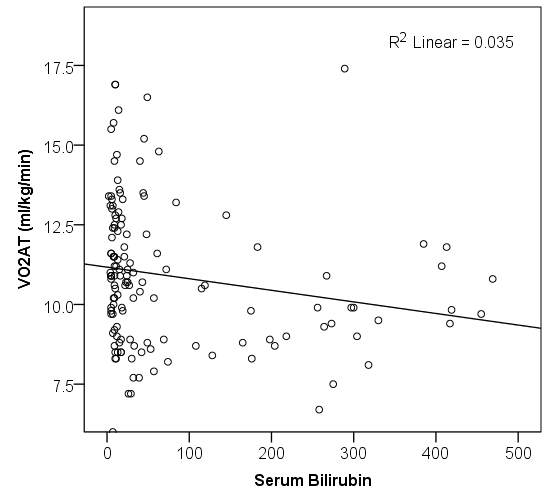
\includegraphics[width=\textwidth]{Figures/cpet_oj_scatter_at_bil}
		\caption{$\dot{V}_{O_2}$AT versus serum bilirubin}
		\label{fig:cpet_oj_scatter_at_bil}
	\end{subfigure}
	\begin{subfigure}{0.48\textwidth}
		\centering
		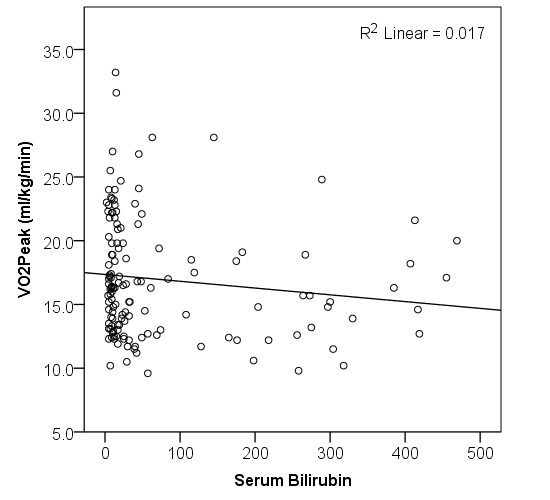
\includegraphics[width=\textwidth]{Figures/cpet_oj_scatter_peak_bil}
		\caption{$\dot{V}_{O_2}$Peak versus serum bilirubin}
		\label{fig:cpet_oj_scatter_peak_bil}
	\end{subfigure}
	
	\caption{Scatter-plot analysis comparing serum bilirubin versus $\dot{V}_{O_2}$AT and $\dot{V}_{O_2}$Peak.}
	\label{fig:cpet_oj_scatter}
	
\end{figure}

\subsection{Preoperative factors related to CPET}
Binary logistic regression analysis was undertaken to assess preoperative clinico-pathological patient factors associated with a low $\dot{V}_{O_2}$AT and low $\dot{V}_{O_2}$Peak. 
On univariate analysis, female sex (HR 2.74, 95\% CI 1.30-5.74, p=0.008), body mass index $>$ 25 (HR 3.09, 95\% CI 1.51-6.32, p=0.002), presence of malignancy (HR 3.59, 95\% CI 1.36-9.43, p=0.010), POSSUM Physiology Score $>$ 14 (HR 2.06, 95\% CI 1.02-4.17, p= 0.044), serum bilirubin $>$ 250 $\mu$mol/l (HR 5.66, 95\% CI 1.87-17.16, p=0.002), haemoglobin $<$ 12 g/dl (HR 2.74, 95\% CI 1.30-5.74, p=0.008) and serum C-reactive protein $>$ 10 mg/l (HR 2.18, 95\% CI 1.06-4.51, p=0.035) were associated with $\dot{V}_{O_2}$AT $<$ 10 ml/kg/min. 
Age, cardiovascular and respiratory comorbidity, PBD, mild jaundice and serum albumin were not significantly related to a low $\dot{V}_{O_2}$AT. 

The statistically significant independent variables with p$<$0.05 were entered into a backward step-wise regression model with $\dot{V}_{O_2}$AT $<$ 10 ml/kg/min as a categorical, binomial, dependent variable. 
Female sex (HR 3.75, 95\% CI 1.57-8.95 p$<$0.005), body mass index $>$ 25 (HR 3.65, 95\% CI 1.61-8.26, p$<$0.005), malignancy (HR 4.02, 95\% CI 1.33-12.16, p$<$0.05) and C-reactive protein $>$ 10 mg/l (HR 2.98, 95\% CI 1.29-6.86, p$<$0.05) were independently related to low $\dot{V}_{O_2}$AT. 
Obstructive jaundice was not related to low $\dot{V}_{O_2}$AT on multivariate analysis. (Table \ref{table:cpet_oj_at_regression})

Binary logistic regression analysis of the relationship between patient factors and low $\dot{V}_{O_2}$Peak ($<$ 16 ml/kg/min) is shown in Table \ref{table:cpet_oj_peak_regression}. 
On both univariate and multivariate analysis, female sex, body mass index $>$ 25 and haemoglobin $<$ 12 g/dl were significantly associated with a low $\dot{V}_{O_2}$Peak. 

\begin{sidewaystable}[p]
	\caption{The relationship between clinico-pathological characteristics and low $\dot{V}_{O_2}$AT ($<$ 10 ml/kg/min) in patients undergoing pancreaticoduodenectomy: Univariate and multivariate binary logistic regression analysis}
	\label{table:cpet_oj_at_regression}
	\setlength{\tabcolsep}{9pt} %sets the space between columns
	\centering
	\begin{tabular}{|l l c| c c c| c c c|}
		\hline
		Variable                   &           & n   & HR   & 95\% CI    & \textit{p} & HR   & 95\% CI    & \textit{p} \\ \hline
		Age (years)                & $\leq$ 65 & 70  &      &            &            &      &            &  \\
		                           & $>$ 65    & 68  & 1.19 & 0.60-2.35  & 0.628      &      &            &  \\
		Sex                        & Male      & 95  &      &            &            &      &            &  \\
		                           & Female    & 43  & 2.74 & 1.30-5.74  & 0.008      & 3.75 & 1.57-8.95  & 0.003      \\
		Body Mass Index ($kg/m^2$) & $\leq$ 25 & 69  &      &            &            &      &            &  \\
		                           & $>$ 25    & 69  & 3.09 & 1.51-6.32  & 0.002      & 3.65 & 1.61-8.26  & 0.002      \\
		Smoking                    & No        & 88  &      &            &            &      &            &  \\
		                           & Yes       & 50  & 1.38 & 0.68-2.79  & 0.378      &      &            &  \\
		Cardiovascular disease     & No        & 78  &      &            &            &      &            &  \\
		                           & Yes       & 58  & 0.82 & 0.41-1.64  & 0.569      &      &            &  \\
		Respiratory disease        & No        & 124 &      &            &            &      &            &  \\
		                           & Yes       & 12  & 2.37 & 0.71-7.91  & 0.159      &      &            &  \\
		Cancer                     & No        & 32  &      &            &            &      &            &  \\
		                           & Yes       & 106 & 3.59 & 1.36-9.43  & 0.010      & 4.02 & 1.33-12.16 & 0.014      \\
		POSSUM Physiology Score    & $\leq$ 14 & 72  &      &            &            &      &            &  \\
		                           & $>$ 14    & 61  & 2.06 & 1.02-4.17  & 0.044      &      &            & 0.164      \\
		Biliary stent              & No        & 56  &      &            &            &      &            &  \\
		                           & Yes       & 49  & 0.69 & 0.32-1.50  & 0.347      &      &            &  \\
		Bilirubin ($\mu$mol/l)     & $\leq$ 17 & 65  &      &            &            &      &            &  \\
		                           & 18-35     & 22  & 1.49 & 0.54-4.16  & 0.444      &      &            & 0.911      \\
		                           & 36-250    & 32  & 2.30 & 0.95-5.56  & 0.064      &      &            & 0.537      \\
		                           & $>$ 250   & 19  & 5.66 & 1.87-17.16 & 0.002      &      &            & 0.443      \\
		Haemoglobin (g/dl)         & $\geq$ 12 & 95  &      &            &            &      &            &  \\
		                           & $<$ 12    & 43  & 2.74 & 1.30-5.74  & 0.008      &      &            & 0.214      \\
		C-reactive protein (mg/l)  & $\leq$ 10 & 90  &      &            &            &      &            &  \\
		                           & $>$ 10    & 46  & 2.18 & 1.06-4.51  & 0.035      & 2.98 & 1.29-6.86  & 0.010      \\
		Albumin (g/l)              & $\geq$ 35 & 65  &      &            &            &      &            &  \\
		                           & $<$ 35    & 73  & 1.53 & 0.76-3.05  & 0.231      &      &            &  \\ \hline
	\end{tabular}
	\medskip
	\caption*{Impaired oxygen consumption at the anaerobic threshold ($\dot{V}_{O_2}$AT $<$ 10 ml/kg/min) was independently associated with female sex, body mass index $>$ 25 $kg/m^2$, presence of cancer and raised preoperative C-reactive protein (CRP) level ($>$ 10mg/l).}
\end{sidewaystable}
\begin{sidewaystable}[p]
	\caption{The relationship between clinico-pathological characteristics and low $\dot{V}_{O_2}$Peak ($<$ 16 ml/kg/min) in patients undergoing pancreaticoduodenectomy: Univariate and multivariate binary logistic regression analysis}
	\label{table:cpet_oj_peak_regression}
	\setlength{\tabcolsep}{9pt} %sets the space between columns
	\centering
	\begin{tabular}{|l l c| c c c| c c c|}
		\hline
		Variable                   &           & n   & HR   & 95\% CI   & \textit{p} & HR   & 95\% CI   & \textit{p} \\ \hline
		Age (years)                & $\leq$ 65 & 70  &      &           &            &      &           &  \\
		                           & $>$ 65    & 68  & 1.50 & 0.77-2.94 & 0.237      &      &           &  \\
		Sex                        & Male      & 95  &      &           &            &      &           &  \\
		                           & Female    & 43  & 7.44 & 3.18-17.4 & $<$0.001   & 7.57 & 3.09-18.5 & $<$0.001   \\
		Body Mass Index ($kg/m^2$) & $\leq$ 25 & 69  &      &           &            &      &           &  \\
		                           & $>$ 25    & 69  & 2.02 & 1.03-3.99 & 0.042      & 2.57 & 1.18-5.63 & 0.018      \\
		Smoking                    & No        & 88  &      &           &            &      &           &  \\
		                           & Yes       & 50  & 1.90 & 0.94-3.85 & 0.073      &      &           &  \\
		Cardiovascular disease     & No        & 78  &      &           &            &      &           &  \\
		                           & Yes       & 58  & 1.68 & 0.85-3.33 & 0.139      &      &           &  \\
		Respiratory disease        & No        & 124 &      &           &            &      &           &  \\
		                           & Yes       & 12  & 2.35 & 0.67-8.21 & 0.181      &      &           &  \\
		Cancer                     & No        & 32  &      &           &            &      &           &  \\
		                           & Yes       & 106 & 2.06 & 0.90-4.69 & 0.085      &      &           &  \\
		POSSUM Physiology Score    & $\leq$ 14 & 72  &      &           &            &      &           &  \\
		                           & $>$ 14    & 61  & 1.76 & 0.89-3.51 & 0.107      &      &           &  \\
		Preop Biliary Drainage     & No        & 56  &      &           &            &      &           &  \\
		                           & Yes       & 49  & 0.91 & 0.42-1.97 & 0.814      &      &           &  \\
		Bilirubin ($\mu$mol/l)     & $\leq$ 17 & 65  &      &           &            &      &           &  \\
		                           & 18-35     & 22  & 2.31 & 0.86-6.19 & 0.096      &      &           &  \\
		                           & 36-250    & 32  & 1.60 & 0.68-3.76 & 0.281      &      &           &  \\
		                           & $>$ 250   & 19  & 2.74 & 0.95-7.90 & 0.062      &      &           &  \\
		Haemoglobin (g/dl)         & $\geq$ 12 & 95  &      &           &            &      &           &  \\
		                           & $<$ 12    & 43  & 2.80 & 1.32-5.93 & 0.007      & 2.43 & 1.05-5.63 & 0.038      \\
		C-reactive protein (mg/l)  & $\leq$ 10 & 90  &      &           &            &      &           &  \\
		                           & $>$ 10    & 46  & 1.42 & 0.69-2.90 & 0.333      &      &           &  \\
		Albumin (g/l)              & $\geq$ 35 & 65  &      &           &            &      &           &  \\
		                           & $<$ 35    & 73  & 1.28 & 0.65-2.49 & 0.476      &      &           &  \\ \hline
	\end{tabular}
	\medskip
	\begin{flushleft}
		Oxygen consumption at peak exercise ($\dot{V}_{O_2}$Peak) $<$ 16 ml/kg/min was independently associated with female sex, body mass index $>$ 25 $kg/m^2$, presence of cancer and raised preoperative C-reactive protein (CRP) level ($>$ 10 mg/l).
	\end{flushleft}
\end{sidewaystable}

\clearpage

\section{Discussion}

The results of the present study demonstrate that obstructive jaundice, even when severe, is not an independent risk factor for poor preoperative cardiopulmonary exercise physiology in patients undergoing pancreaticoduodenectomy. 
The results also demonstrate that obstructive jaundice is associated with elevated preoperative systemic inflammation with the severity of systemic inflammation related to the severity of the jaundice.
The results also appear to suggest that there may be multiple other determinants of aerobic capacity including female sex, body mass index, haemoglobin, presence of cancer and systemic inflammation.

%History of CPET
The use of CPET in preoperative risk prediction was first made popular over two decades ago by Older and co-workers \parencite{older_preoperative_1993}. 
Since then cardiopulmonary exercise testing has been reported to be useful in identifying high risk patients prior to major general \parencite{snowden_submaximal_2010}, pancreatic \parencite{ausania_effects_2012}[Chapter \ref{ch_cpet_outcomes} of this thesis], oesophagogastric \parencite{nagamatsu_preoperative_2001} as well as vascular \parencite{carlisle_mid-term_2007} surgery. 
Cardiopulmonary exercise testing is superior to conventional measures of fitness due to the dynamic nature of the test that evaluates the adequacy of oxygen delivery to tissues under physiological stress. 
However, the factors responsible for poor aerobic capacity in surgical patients have not been adequately studied. 
The present study aimed to address this in patients undergoing major pancreatic surgery.

%History of jaundice - reason for PBD
Experimental and animal studies have shown that obstructive jaundice was associated with myocardial depression \parencite{green_jaundiced_1986}, poor myocardial response to inotropic stimulation \parencite{lumlertgul_jaundiced_1991}, impaired sympathetic baroreflex sensitivity \parencite{song_baroreflex_2009} and deranged atrial natriuretic peptide levels \parencite{pereira_increased_1994,gallardo_increased_1998}. 

Historically, obstructive jaundice has also been reported to be associated with adverse haemodynamic events in patients undergoing major surgery. 
Intra-operative blood loss, postoperative hypotension, increased susceptibility to shock and renal dysfunction were more common in patients with obstructive jaundice \parencite{dixon_factors_1983, pain_perioperative_1985, green_systemic_1995}.
A recent review noted that bile acids had a complex range of receptor mediated effects on the cardiovascular system \parencite{khurana_bile_2011}. 
Moreover, some of these effects appear to be partly reversible by biliary drainage as demonstrated by Padillo and co-workers \parencite{padillo_improved_2001}.

These observations led to routine pre-operative biliary drainage being recommended in all jaundiced patients before undertaking major surgery. 
Pancreaticoduodenectomy was described by Whipple initially as a two-stage operation, with the first stage involving a cholecysto-gastrostomy aimed at relieving biliary obstruction before undertaking the resection at a later second operation \parencite{whipple_treatment_1935}.

%Reasons for not doing PBD
However, several recent studies have reported that PBD is associated with increased incidence of complications and that surgery in the jaundiced patients is safe.
Pitt and co-workers in a prospective randomised trial compared outcomes in jaundiced patients undergoing surgery with or without PBD. They reported that PBD was associated with increased cost without any decrease in postoperative complications \parencite{pitt_does_1985}. 
A recent meta-analysis \parencite{sewnath_meta-analysis_2002} pooled data from 5 randomised controlled trials comparing surgery with PBD versus surgery without drainage.
The authors concluded that PBD not only did not improve postoperative complication rates or mortality but resulted in a higher overall complication rate due to the morbidity associated with the procedure itself. 
These findings have been reproduced in a more recent multicenter, randomised trial \parencite{van_der_gaag_preoperative_2010}.
A recent Cochrane Collaboration review of six trials including 520 patients concluded that PBD may be associated with serious adverse events and must not be performed routinely outside trial settings \parencite{wang_preoperative_2008}.

%CPET vs Jaundice
In the present study, obstructive jaundice was not independently related to $\dot{V}_{O_2}$AT or $\dot{V}_{O_2}$Peak.
There was only a weak negative correlation between serum bilirubin and $\dot{V}_{O_2}$AT in our cohort.
These findings are similar to those of Parker and co-workers who reported that there was only a weak negative correlation between serum bilirubin and  $\dot{V}_{O_2}$Peak (Pearson's $\rho$ -0.21, p=0.02) and no correlation with $\dot{V}_{O_2}$AT ($\rho$ = -0.15, p=NS) in patients undergoing pancreaticoduodenectomy \parencite{parker_serum_2014}. 
Junejo and co-workers studied oxygen extraction in 9 jaundiced patients during cardiopulmonary exercise test by placing catheters within the femoral vein and reported that oxygen extraction was normal during cardiopulmonary exercise even in the presence of jaundice \parencite{junejo_peripheral_2014}

Taken together, these results appear to suggest that preoperative biliary drainage and resolution of jaundice are unlikely to improve aerobic capacity and cardiopulmonary physiology in these patients.
\todo{Remove this conclusion not based on thesis}

%Obstructive jaundice and systemic inflammation
However, jaundice was associated with elevated preoperative systemic inflammation as measured by C-reactive protein levels and serum albumin. 
Obstructive jaundice is known to be associated with wide ranging abnormalities of both humoral and innate immune systems \parencite{nehez_compromise_2002, padillo_cytokines_2001, scott-conner_pathophysiology_1994}. 
It is unclear if this preoperative immune dysfunction continues after surgery as an abnormal postoperative systemic inflammatory response and this is explored further in Chapter \ref{ch_pre_post_sirs}.
However, studies suggest that the immunological abnormalities associated with obstructive jaundice did not improve after biliary drainage \parencite{kimmings_endotoxin_2000}.

Elevated preoperative CRP was also independently associated with a low $\dot{V}_{O_2}$AT suggesting that impaired aerobic capacity may be associated with a systemic inflammatory response.
This finding is similar to that reported by Sultan and co-workers who found that low $\dot{V}_{O_2}$AT was independently associated with an elevated preoperative neutrophil-lymphocyte ratio in patients undergoing colorectal surgery \parencite{sultan_cardiopulmonary_2014}.

%CPET vs Haemoglobin
The association between low haemoglobin and low $\dot{V}_{O_2}$Peak would appear to be more easily explained since the oxygen carrying capacity of blood depends on haemoglobin concentration.  
Indeed, the linear relationship between oxygen consumption during exercise and haemoglobin concentration has been shown both in disease states \parencite{agostoni_relationship_2010} as well as in healthy volunteers \parencite{dellweg_cardiopulmonary_2008}.
This would suggest that maintaining optimal haemoglobin levels in the perioperative period will improve oxygen delivery and perhaps outcome as well. 
Excessive intra-operative blood loss has been reported to be associated with postoperative complications \parencite{pratt_risk_2008} and this may in part be due impaired oxygen delivery at a time of maximal physiological burden.

%CPET vs BMI, Sex
In the present study, it was of interest that $\dot{V}_{O_2}$, both at anaerobic threshold and at peak exercise, was significantly lower in females as well as in patients with  a high body mass index.
The basis of this relationship is not clear and may be related to body composition differences between these groups.
However, such an association has been previously reported \parencite{horwich_relationship_2009}.
This may reflect the difficulty in obtaining accurate $\dot{V}_{O_2}$ values in obese patients as a result of the calculations involved rather than due to true cardiopulmonary dysfunction. 
Other authors have suggested that different thresholds for CPET parameters may have to be considered in obese patients to improve risk-prediction \parencite{donnelly_criteria_1990,hulens_exercise_2001}.
Presence of cancer was also an independent predictor of low $\dot{V}_{O_2}$AT.
Sarcopenia is associated with reduced aerobic capacity \parencite{evans_sarcopenia_1993} and is common in pancreatic cancer \parencite{joglekar_sarcopenia_2015}.
$\dot{V}_{O_2}$AT and $\dot{V}_{O_2}$Peak must be interpreted with caution in these patient groups.
This is the subject of further study in Chapter \ref{ch_bodycomp}.

%\subsection{Conclusion}
In conclusion, obstructive jaundice, including severe obstructive jaundice did not affect preoperative cardiopulmonary exercise physiology. 
Therefore, preoperative biliary drainage cannot be expected to improve aerobic capacity in patients undergoing pancreaticoduodenectomy.
Both obstructive jaundice and low $\dot{V}_{O_2}$AT were associated with elevated preoperative systemic inflammation and provide further evidence of the role of jaundice and impaired aerobic capacity in immune dysregulation in these patients.

%% Chapter 04
\chapter{An investigation into the relationship between cardiopulmonary exercise testing and body composition in patients undergoing major pancreatic surgery.}
\label{ch_bodycomp}

\lhead{Chapter \ref{ch_bodycomp}. \emph{CPET and Body Composition}} % This is for the header on each page - perhaps a shortened title

\clearpage
%----------------------------------------------------------------------------------------
\todo{Consider including relationship with systemic inflammation} 

zotero - richards-relationships-2012

\section{Introduction}
Major abdominal surgery especially for pancreatic disease is associated with significant morbidity and mortality. Patient selection is as important as identifying surgical treatable pathology in ensuring optimal outcomes \parencite{balthazar_acute_2002}.

\subsection{Role of preoperative CPET}
The role of cardiopulmonary exercise testing in the preoperative evaluation and risk assessment/stratification of patients undergoing major thoracic and abdominal surgery has become well established. A number of studies have shown that poor aerobic fitness demonstrated by a low $\dot{V}_{O_2}$AT or low $\dot{V}_{O_2}$Peak or both as measured at cardiopulmonary exercise testing is associated with increased morbidity and mortality after major surgery including bariartic\parencite{mccullough_cardiorespiratory_2006}, pancreatic\parencite{ausania_effects_2012}[Chapter \ref{ch_cpet_outcomes}], liver \parencite{epstein_aerobic_2004}, cardiothoracic\parencite{brunelli_risk_2010, campione_oxygen_2010,torchio_exercise_2010} and abdominal aortic aneurysm surgery \parencite{carlisle_mid-term_2007,thompson_cardiopulmonary_2011}. CPET is now routinely used as part of the preoperative processes used to select patients for surgery as well as to help in decision making regarding preoperative care including the need for additional tests, preoperative and intraoperative optimisation, admission to critical care and postoperative care.
Patients are sometimes denied surgery if their performance at cardiopulmonary exercise testing is felt to be poor based on currently available evidence.

\subsection{The pathophysiological basis of CPET}
Aerobic fitness, as defined by the ability to perform physical exercise, is dependant on and often limited by the ability of the cardiorespiratory and circulatory systems (henceforth simply the cardiorespiratory system) to supply O2 to skeletal muscles at times of increased demand as well as remove the main end product of aerobic metabolism, namely CO2. Several factors play an important role in this increased response of the cardiorespiratory system. The most important factor is an increase in cardiac output which in healthy adults can increase by upto six-fold during exercise. Aside from increased stroke volume and heart rate, the redistribution of blood volume from the splanchnic circulation increases venous return to the heart. A consequent increase in pulmonary blood flow and skeletal blood flow occurs which in turn is assisted by vasodilation in these circulatory beds.

Oxygenation of the increased pulmonary blood flow and removal of the excess CO2 generated by aerobic exercise is effected by increased minute ventilation as a result of increase in its constituent factors namely respiratory rate and tidal volume. Oxygenation of skeletal muscle is further dependant on numerous other factors including the oxygen carrying capacity of blood (primary determinant being haemoglobin), adequate peripheral circulation and the ability of the mitochondria within the skeletal muscle to utilise the oxygen that is being delivered to them. 

It is clear that limitations in the patient's physiology resulting in inadequate or inappropriate response in any of the above mentioned factors will result in overall limitation of their aerobic fitness. Cardiopulmonary exercise testing allows the accurate measurement of most of these factors either directly or indirectly during dynamic exercise thus allowing identifying not only limitations in aerobic fitness but also the cause for such limitation. 

\subsection{Factors influencing aerobic fitness}
A low $\dot{V}_{O_2}$ has universally been attributed to low aerobic fitness due to an inadequate response of the cardiovascular and respiratory systems to increased oxygen demand during exercise. This is often thought to be due to cardiorespiratory disease, overt or sub-clinical. Occasionally, other factors such as anaemia, peripheral vascular disease and rarely, mitochondrial diseases have been recognised as factors contributing to low $\dot{V}_{O_2}$ or abnormalities in other parameters measured at cardiopulmonary exercise testing but these causes are less common in patients undergoing major abdominal surgery.

The most common parameters used to quantify perioperative risk in surgical patients are oxygen consumption at the anaerobic threshold ($\dot{V}_{O_2}$AT) and at peak exercise capacity ($\dot{V}_{O_2}$Peak). Conventionally these have been reported as per weight ratios (ml/kg/min) to allow comparison between patients. However, numerous studies on cardiorespiratory exercise physiology have reported that normalising $\dot{V}_{O_2}$ using total body weight leads to spurious correlation errors unfairly penalising obese subjects \parencite{seltzer_body_1940, tanner_fallacy_1949, toth_examination_1993, batterham_modeling_1999, goran_total_2000, krachler_cardiopulmonary_2014} 

\subsection{Aims}
In chapter \ref{ch_cpet_outcomes}, we reported that low $\dot{V}_{O_2}$AT in patients undergoing pancreaticoduodenectomy was associated with increased incidence of postoperative pancreatic fistula and prolonged hospital stay. We also reported that patients with a $\dot{V}_{O_2}$AT less than 10 ml/kg/min were less likely to receive postoperative adjuvant chemotherapy as a result of postoperative complications, prolonged hospital stay and possibly due to lack of physiological reserve after surgery. However, we also observed that high BMI was associated with a low $\dot{V}_{O_2}$AT independent of all other clinicopathological characteristics. Moreover, most of our patients did not have overt cardiac or respiratory comorbidity to explain the very low levels of $\dot{V}_{O_2}$AT.

The aim of the present study was to explore the association between body composition, total body weight and the physiological parameters measured at cardiopulmonary exercise testing.

\clearpage
\section{Methods}

\subsection{Patients}
Patients scheduled to undergo pancreaticoduodenectomy for malignant or benign disease involving the head of the pancreas and periampullary region between August 2008 and October 2010 were included in this study. All data were recorded in a prospectively maintained database. Data was collected on demographics, preoperative clinicopathological characteristics including blood tests, body mass index, weight, height and the underlying surgical pathology. Detailed breath-by-breath data on a variety of physiological and gas-exchange parameters measured at cardiopulmonary exercise testing were also collected from a prospectively maintained database. Cardiopulmonary exercise testing methodolgy is discussed in Section \ref{sec:cpx_method} (p\pageref{sec:cpx_parameters})and a description of the parameters measured at cardiopulmonary exercise testing is provided in Section \ref{sec:cpx_parameters} (p\pageref{sec:cpx_parameters}).

\subsection{Calculation of body composition}
\label{sec:bodycomp_calculation}
Computed tomography of the abdomen, performed as part of the routine preoperative staging, was used to calculate body composition based on previously published and well established methods \parencite{bredella_comparison_2010,shen_total_2004}.

%http://regionstraumapro.com/post/16349545265 - Excellent description of CT window width(W) and level/center(C)
The coronal and sagittal reconstructions were used to accurately identify the L3 and L4 vertebrae. The CT window width (W) was set at 400 and the level/center (C) was set at 40. This allowed tissue between -160 HU and +240 HU to be represented in grayscale with adequate contrast between tissues of interest. The cross-sectional images at these levels where then exported as gray-scale bitmap images. The scale in millimeters was included with every image. A representative image is shown in Fig. 1.The GNU Image Manipulation Program (GIMP), an advanced, free, open-source, raster graphics editor was used for analysis of all images (www.gimp.org). The use of GIMP to analyse cross-sectional imaging for body composition has been described previously although by using a different technique to what has been employed by us \parencite{anblagan_measurement_2013}.

The first step involved converting the bitmap images into JPEG images using lossy compression set at 85\% to minimise sharp transitions between grey areas of very similar colour values. This allowed more consistent selection of contiguous areas of similar grey shades. 

The next step involved standardising the scale of all images by dividing the length of the scale on every image by the number of pixels along the scale thus providing a length in millimetres for each pixel in each image. As pixels on a CT image are square, the area of each pixel was calculated as a square of its length. 

The Fuzzy Select (Magic Wand) tool was used to select contiguous areas of similar colour while simultaneously using visual confirmation that the correct anatomical structures had been selected without overspill into unwanted areas. The number of pixels within the selection was obtained using the 'Histogram' dialog window and entered into an excel spreadsheet against the selected area of interest. The area in mm2 was calculated by multiplying the number of pixels by the area of each pixel.

\textbf{Selecting tissue compartments}:

The sequence of steps followed to calculate the area of each tissue compartment is depicted in Fig. \ref{fig:bc_ct_gimp} on p \pageref{fig:bc_ct_gimp}. The total cross-sectional area of the abdomen at the level of L3/L4 was calculated by first selecting all the empty space outside the image followed by inverting this selection. This is depicted in Fig. \ref{fig:bc_ct_csa}. Subcutaneous fat in the image was selected using the Fuzzy Select tool (if necessary by choosing multiple times and removing any unnecessary areas) as depicted in Fig. \ref{fig:bc_ct_sat}. The same process was repeated for visceral adipose tissue and skeletal muscle as depicted in Fig. \ref{fig:bc_ct_vat} and Fig. \ref{fig:bc_ct_sm} respectively. Every selection was visually confirmed for anatomical accuracy by using the layer selection tool to inspect the area under selection as shown in the insets in each of the images.
%CT slices images x 4
\begin{figure}[htbp]
	\centering
	\begin{subfigure}{0.45\textwidth}
		\centering
		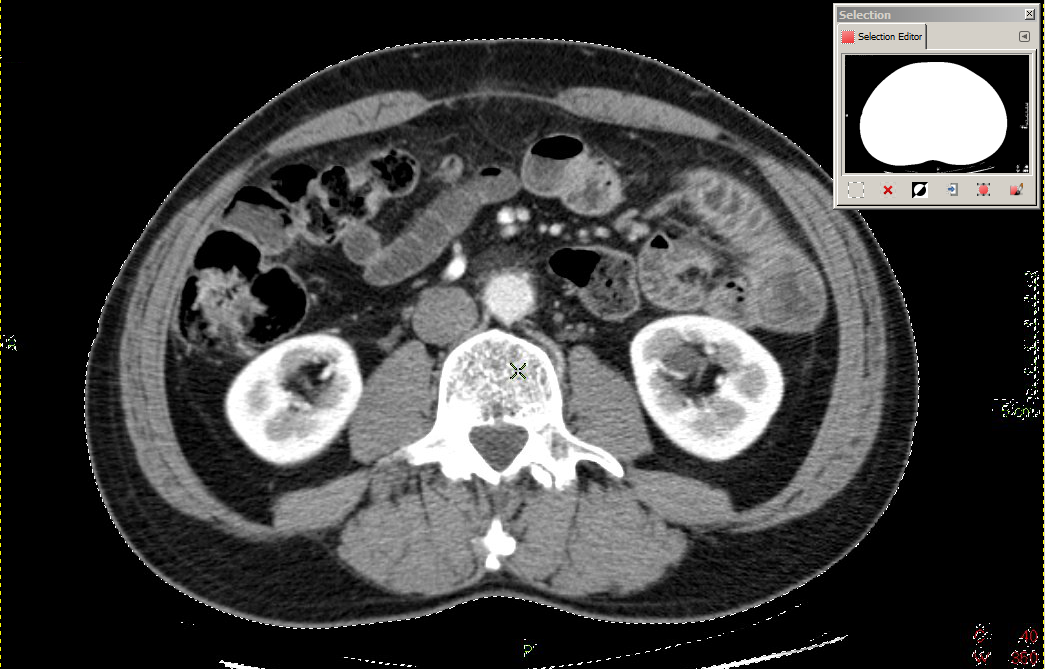
\includegraphics[width=\textwidth]{Figures/bc_ct_csa}
		\caption{Total Cross-sectional Area}
		\label{fig:bc_ct_csa}
	\end{subfigure}
	\begin{subfigure}{0.45\textwidth}
		\centering
		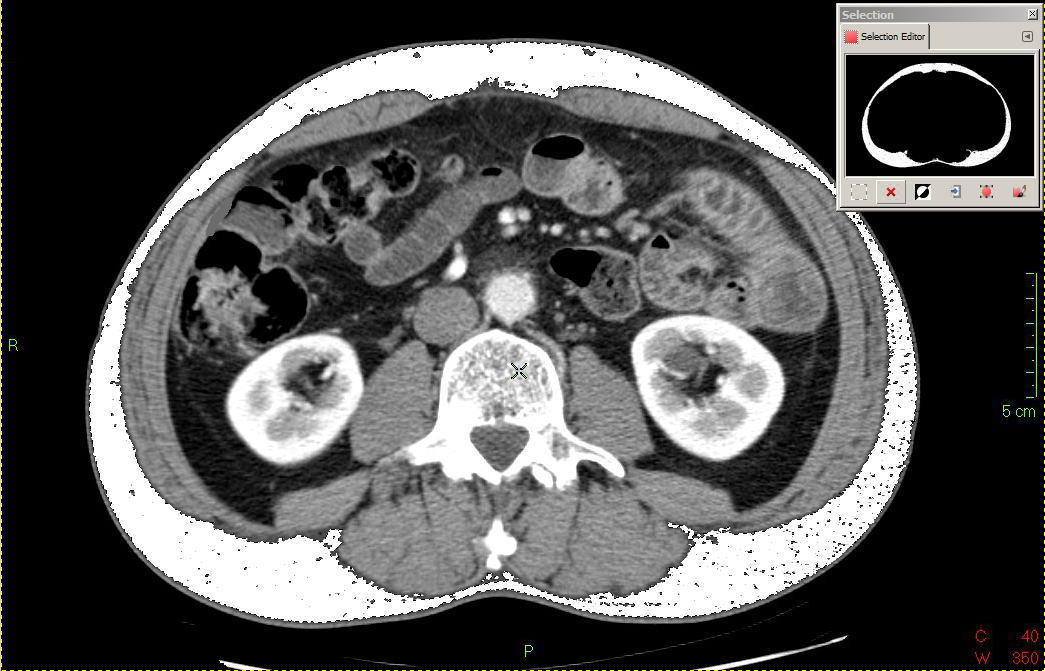
\includegraphics[width=\textwidth]{Figures/bc_ct_sat}
		\caption{Subcutaneous Adipose Tissue$^*$}
		\label{fig:bc_ct_sat}
	\end{subfigure}
	\hfill
	\begin{subfigure}{0.45\textwidth}
		\centering
		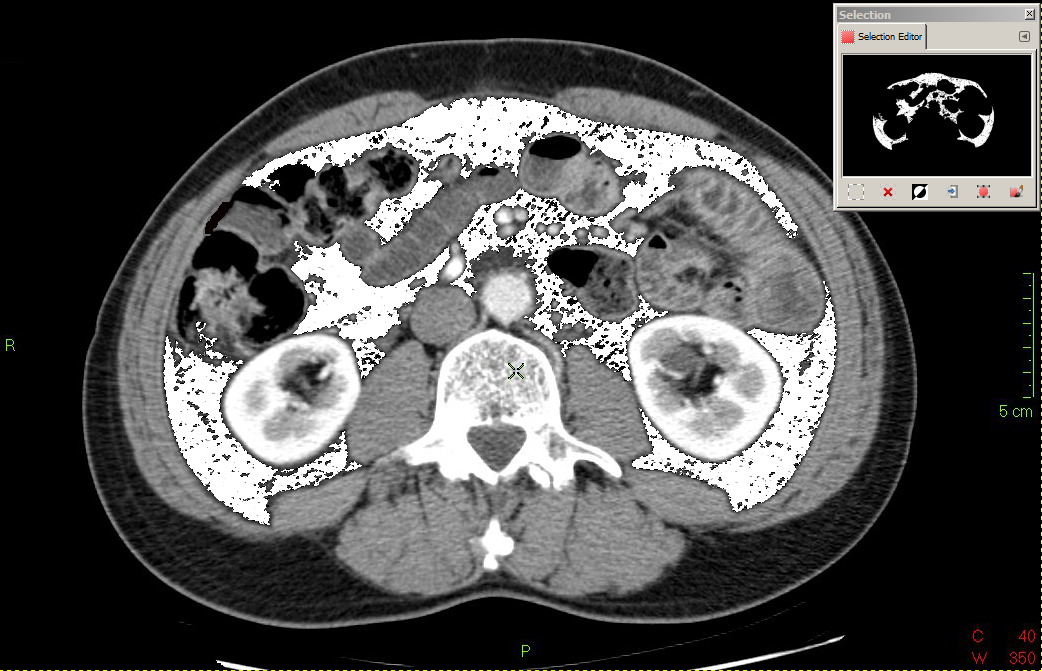
\includegraphics[width=\textwidth]{Figures/bc_ct_vat}
		\caption{Visceral Adipose Tissue$^*$}
		\label{fig:bc_ct_vat}
	\end{subfigure}
	\begin{subfigure}{0.45\textwidth}
		\centering
		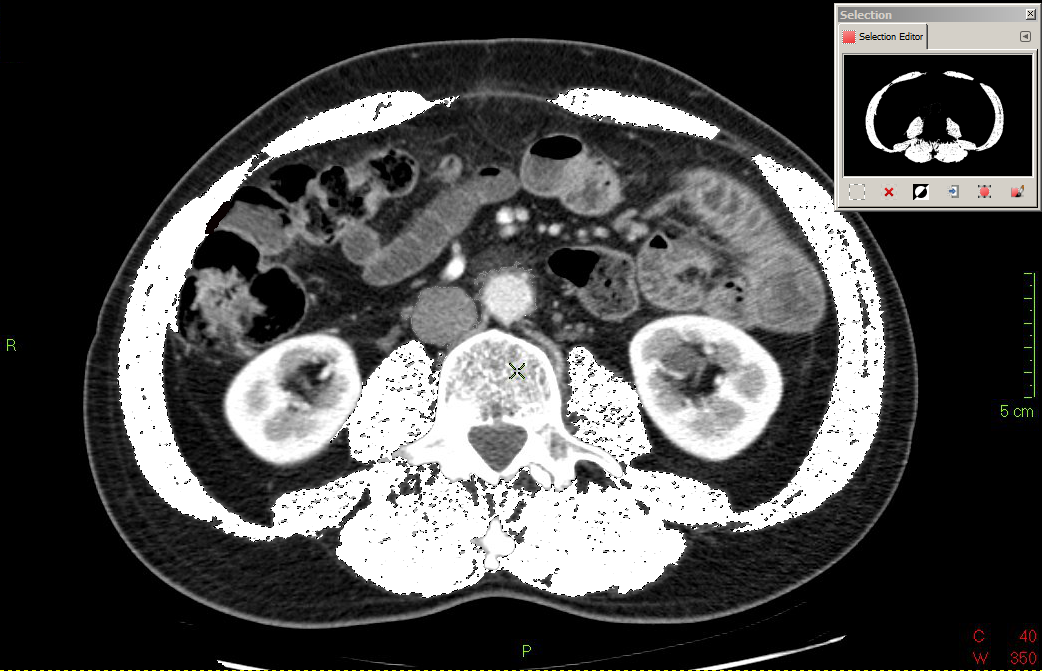
\includegraphics[width=\textwidth]{Figures/bc_ct_sm}
		\caption{Skeletal Muscle$^*$}
		\label{fig:bc_ct_sm}
	\end{subfigure}
	
	\caption{Selection of components of body composition from CT images using GIMP.}($^*$ The selected area has been removed for representation purposes. The inset confirms the area selected.)
	\label{fig:bc_ct_gimp}
	
\end{figure}

\subsection{Cardiopulmonary exercise testing}
All patients performed cardiopulmonary exercise testing on a cycle ergometer as described in Section \ref{sec:cpx_method}. Raw data of all breath-by-breath parameters averaged every 10 seconds was collected for analysis. The first three minutes of the recorded data were during the rest period when the patients were on the exercise bike but did not exercise. The average of each parameter measured between the first and second minute (6 readings) was treated as the rest value. Anaerobic threshold was identified using previously established methods and all corresponding parameters at this point were recorded \parencite{beaver_new_1986,sue_metabolic_1988}. Peak exercise was identified by the maximum oxygen consumption recorded towards the end of the exercise period and all other parameters recorded at this point were considered as peak exercise values. 

\subsection{Statistics}

All analyses were performed using the SPSS statistical package for Microsoft Windows (version 22 ). Comparison between body composition and cardiopulmonary exercise testing parameters was done using Partial correlations controlling for the effect of gender (and/or age). All p-values reported are two-sided. The relationship between body composition and preoperative clinico-pathological characteristics (as categorical variables) was analysed using the Mann-Whitney U test for variables with two categories or the Kruskal-Wallis test for variables with more than two categories. Previously established cut-offs were used for categorising continuous variables where applicable. The level of significance was set at $p<0.05$.

\clearpage
\section{Results}

\subsection{Body composition and Clinico-pathological characteristics}
Eighty-two patients (52 male) were included in the study. 
The clinico-pathological characteristics of the study patients and their relationship to body composition is shown in Table \ref{table:bc_clinical} on page \pageref{table:bc_clinical}. 
There were several significant associations between clinico-pathological variables and body composition as shown in this table. 
Females had a greater area of subcutaneous adipose tissue (223.9 versus 141.6 cm$^2$, p$<$0.001) but less visceral adipose tissue (79.1 versus 174.9 cm$^2$, p$<$0.001).
However, there was no difference in the total adipose tissue area between men and women (316.6 versus 303.0 cm$^2$, p=0.665).
Skeletal muscle area was greater in males than in females (141.3 versus 99.7 cm$^2$).

Patients from more deprived areas of Scotland as defined by the Scottish Index of Multiple Deprivation (SIMD) had a greater amount of subcutaneous adipose tissue (p=0.041) but no difference in the other body composition parameters.
Hypoalbuminemia was associated with less visceral adipose tissue (p=0.013) and less skeletal muscle area that did not reach statistical significance (p=0.054). 
Anaemia (haemoglobin $<$ 12 g/dl) was associated with increased adiposity in the subcutaneous plane and reduced skeletal muscle area. 
	%%Table 1
\begin{sidewaystable}[p]
 \caption{Body composition parameters distributed by sex in patients undergoing major pancreatic surgery.}
 \label{table:bc_sex_specific_distrib}
 \renewcommand{\arraystretch}{1.2} %Increases space between rows
 %\setlength{\tabcolsep}{9pt} %sets the space between columns
 \centering
 \begin{tabular}{|l|c c c | c c c |c|}
 	\hline
 	                                                  &       \multicolumn{3}{c}{Male}       &       \multicolumn{3}{c}{Female}       & p        \\
 	                                                  &  Mean (SD)   & Range       & n(\%)   & Mean (SD)    & Range       & n(\%)     &  \\ \hline
 	\textbf{Body Mass Index}                          &  26.1 (3.9)  & 18.7-37.6   &         & 24.9 (3.5)   & 18.4-32.4   &           &  \\
 	Underweight ($<$18.5)                             &              &             & 0 (0)   &              &             & 1 (3)     &  \\
 	Normal (18.5-24.9)                                &              &             & 23 (44) &              &             & 15 (50)   &  \\
 	Overweight (25.0-29.9)                            &              &             & 20 (39) &              &             & 11 (37)   &  \\
 	Obese ($>$30)                                     &              &             & 9 (17)  &              &             & 3 (10)    &  \\ \hline
 	\textbf{Total fat index (cm$^2$/m$^2$)}           & 106.7 (55.7) & 30.4-319.1  &         & 118.8 (65.7) & 24.3-357.7  &           & 0.408    \\
 	Sex-specific tertile "Low"                        & 51.4 (14.9)  & 30.4-74.8   & 17 (33) & 61.6 (25.6)  & 24.3-89.6   & 10 (33.3) &  \\
 	Sex-specific tertile "Medium”                     & 98.9 (17.5)  & 75.1-129.1  & 17 (33) & 111.2 (11.1) & 93.0-124.7  & 10 (33.3) &  \\
 	Sex-specific tertile "High”                       & 166.2 (44.2) & 130.3-319.1 & 18 (34) & 183.6 (69.2) & 125.1-357.7 & 10 (33.3) &  \\ \hline
 	\textbf{Subcutaneous fat index (cm$^2$/m$^2$) }   & 47.4 (31.7)  & 13.7-202.8  &         & 87.8 (51.4)  & 20.8-293.7  &           & $<$0.001 \\
 	Sex-specific tertile "Low”                        &  22.6 (6.8)  & 13.7-31.5   & 17 (33) & 49.5 (17.5)  & 20.8-68.3   & 10 (33.3) &  \\
 	Sex-specific tertile "Medium”                     &  40.4 (5.0)  & 32.2-49.1   & 17 (33) & 77.5 (5.2)   & 71.1-89.3   & 10 (33.3) &  \\
 	Sex-specific tertile "High”                       & 77.5 (36.4)  & 50.2-202.8  & 18 (34) & 136.4 (61.7) & 89.5-293.7  & 10 (33.3) &  \\ \hline
 	\textbf{Visceral fat index (cm$^2$/m$^2$)}        & 59.3 (34.6)  & 9.1-164.4   &         & 31.0 (20.7)  & 0.9-82.5    &           & $<$0.001 \\
 	Sex-specific tertile "Low”                        &  23.0 (8.9)  & 9.1-38.1    & 17 (33) & 10.4 (7.9)   & 0.9-20.2    & 10 (33.3) &  \\
 	Sex-specific tertile "Medium”                     & 54.8 (12.7)  & 38.4-77.4   & 17 (33) & 26.9 (5.8)   & 20.8-35.5   & 10 (33.3) &  \\
 	Sex-specific tertile "High”                       & 97.7 (21.6)  & 79.3-164.4  & 18 (34) & 55.8 (10.9)  & 46.7-82.5   & 10 (33.3) &  \\ \hline
 	\textbf{Skeletal muscle fat index (cm$^2$/m$^2$)} &  47.9 (8.8)  & 30.2-72.5   &         & 38.8 (5.3)   & 24.9-49.9   &           & $<$0.001 \\
 	Sex-specific tertile "Low”                        &  38.5 (4.2)  & 30.2-43.8   & 17 (33) & 32.9 (3.3)   & 24.9-36.2   & 10 (33.3) &  \\
 	Sex-specific tertile "Medium”                     &  47.8 (2.1)  & 44.5-51.1   & 17 (33) & 39.5 (1.0)   & 37.8-40.6   & 10 (33.3) &  \\
 	Sex-specific tertile "High”                       &  56.9 (6.1)  & 51.3-72.5   & 18 (34) & 43.9 (3.4)   & 40.9-49.9   & 10 (33.3) &  \\ \hline
 \end{tabular}
\end{sidewaystable}
	%%Table 1
\begin{sidewaystable}[p]
	\tiny
	\caption{The relationship between body composition and clinico-pathological characteristics of patients undergoing major pancreatic surgery.}
	\label{table:bc_clinical}
	%\renewcommand{\arraystretch}{1.2} %Increases space between rows
	\setlength{\tabcolsep}{9pt} %sets the space between columns
	\centering
	\begin{tabular}{|l l| c c | c c| c c | c c |c c |}
		                    &           & \multicolumn{2}{c}{Body Mass} & \multicolumn{2}{c}{Total fat} & \multicolumn{2}{c}{Subcutaneous fat } & \multicolumn{2}{c}{Visceral fat} & \multicolumn{2}{c}{Skeletal Muscle} \\
		                    &           & index           & p           & index        & p              & index        & p                      & index        & p                 & index        & p                    \\
		                    &           & norm/Over/Obese &             & low/med/high &                & low/med/high &                        & low/med/high &                   & low/med/high &  \\
		Age                 & $<$65     & 19/10/6         & 0.752       & 13/12/10     & 0.353          & 16/7/12      & 0.230                  & 11/14/10     & 0.699             & 12/8/15      & 0.486                \\
		                    & $\geq$65  & 19/21/6         &             & 14/15/18     &                & 11/20/16     &                        & 16/13/18     &                   & 15/19/13     &  \\
		SMID                & 0         & 27/18/4         & 0.053       & 22/11/16     & 0.066          & 19/15/15     & 0.211                  & 21/13/15     & 0.094             & 22/12/15     & 0.129                \\
		                    & 1         & 6/8/6           &             & 3/9/9        &                & 5/7/9        &                        & 3/10/8       &                   & 4/9/8        &  \\
		Pathology           & Benign    & 7/2/1           & 0.239       & 5/1/4        & 0.646          & 4/4/2        & 0.385                  & 4/2/4        & 0.960             & 7/1/2        & 0.036                \\
		                    & Malignant & 31/29/11        &             & 22/26/24     &                & 23/23/26     &                        & 23/25/24     &                   & 20/26/26     &  \\
		$\dot{V}_{O_2}$AT   & $\geq$ 10 & 23/12/3         & 0.010       & 20/10/9      & 0.002          & 16/13/10     & 0.082                  & 17/14/8      & 0.011             & 15/11/13     & 0.506                \\
		                    & $<$ 10    & 15/19/9         &             & 7/17/19      &                & 11/14/18     &                        & 10/13/20     &                   & 12/16/15     &  \\
		$\dot{V}_{O_2}$Peak & $\geq$ 16 & 21/12/1         & 0.002       & 18/11/6      & 0.001          & 14/14/7      & 0.044                  & 17/13/5      & 0.001             & 13/10/12     & 0.699                \\
		                    & $<$ 16    & 17/19/11        &             & 9/16/22      &                & 13/13/21     &                        & 10/14/23     &                   & 14/17/16     &  \\
		CRP                 & $\leq$ 10 & 24/18/7         & 0.556       & 16/17/17     & 0.915          & 18/18/14     & 0.205                  & 15/17/18     & 0.511             & 17/15/18     & 0.915                \\
		                    & $>$ 10    & 14/13/5         &             & 11/10/11     &                & 9/9/14       &                        & 12/10/10     &                   & 10/12/10     &  \\
		Albumin             & $\geq$ 35 & 14/14/4         & 0.777       & 10/8/14      & 0.321          & 9/14/9       & 0.915                  & 9/9/14       & 0.205             & 13/9/10      & 0.352                \\
		                    & $<$ 35    & 24/17/8         &             & 17/19/14     &                & 18/13/19     &                        & 18/18/14     &                   & 14/18/18     &  \\
		Haemglobin          & $\geq$ 12 & 26/16/8         & 0.777       & 20/13/17     & 0.321          & 15/21/14     & 0.658                  & 17/17/16     & 0.658             & 16/15/19     & 0.511                \\
		                    & $<$ 12    & 12/15/4         &             & 7/14/11      &                & 12/6/14      &                        & 10/10/12     &                   & 11/12/9      &  \\
		PPS                 & $\leq$ 14 & 16/18/7         & 0.136       & 12/12/17     & 0.228          & 8/19/14      & 0.140                  & 14/12/15     & 0.893             & 13/15/13     & 0.893                \\
		                    & $>$ 14    & 22/13/5         &             & 15/15/11     &                & 19/8/14      &                        & 13/15/13     &                   & 14/12/15     &  \\
		Cardiac             & No        & 25/10/7         & 0.112       & 18/13/12     & 0.080          & 17/14/12     & 0.138                  & 20/10/13     & 0.043             & 21/12/10     & 0.002                \\
		disease             & Yes       & 13/21/5         &             & 9/14/16      &                & 10/13/16     &                        & 7/17/15      &                   & 6/15/18      &  \\
		Respiratory         & No        & 32/27/12        & 0.239       & 22/24/26     & 0.201          & 22/24/26     & 0.201                  & 23/23/26     & 0.385             & 25/23/24     & 0.442                \\
		disease             & Yes       & 6/4/0           &             & 5/3/2        &                & 5/3/2        &                        & 4/4/2        &                   & 2/4/4        &
	\end{tabular}
\end{sidewaystable}

		
	%Table 1
\begin{sidewaystable}[p]
\caption{The relationship between body composition and clinico-pathological characteristics of patients undergoing major pancreatic surgery.}
\label{table:bc_clinical}
\centering
\begin{tabular}{l c c | c c c | c c c | c c c}
	           &           &    & CSA   &       &          & TAT   &       &          & SM    &      &  \\
	           &           & n  & Mean  & SD    & p        & Mean  & SD    & p        & Mean  & SD   & p        \\ \hline
	Age        & $<$ 65    & 35 & 688.6 & 192.8 & 0.386    & 297.0 & 178.5 & 0.309    & 128.7 & 29.4 & 0.590    \\
	           & $\geq$ 65 & 47 & 704.3 & 150.6 &          & 322.7 & 156.6 &          & 124.1 & 31.3 &  \\
	Gender     & M         & 52 & 738.4 & 171.2 & $<$0.001 & 316.6 & 170.8 & 0.665    & 141.3 & 26.1 & $<$0.001 \\
	           & F         & 30 & 626.9 & 141.6 &          & 303.0 & 159.3 &          & 99.7  & 15.6 &  \\
	BMI        & $\leq$ 25 & 39 & 579.9 & 103.6 & $<$0.001 & 205.9 & 97.0  & $<$0.001 & 114.6 & 26.6 & 0.002    \\
	           & 25-30     & 31 & 754.0 & 109.4 &          & 350.6 & 99.6  &          & 136.0 & 30.4 &  \\
	           & $>$ 30    & 12 & 934.6 & 145.4 &          & 554.6 & 185.9 &          & 137.6 & 30.9 &  \\
	SMID       & $>$ 3     & 49 & 684.4 & 163.1 & 0.366    & 288.7 & 175.5 & 0.040    & 123.2 & 31.6 & 0.380    \\
	           & $\leq$ 3  & 21 & 718.5 & 187.2 &          & 365.7 & 165.0 &          & 128.2 & 31.9 &  \\
	Pathology  & Benign    & 10 & 737.9 & 228.4 & 0.766    & 352.8 & 278.1 & 0.955    & 122.4 & 24.0 & 0.788    \\
	           & Malignant & 72 & 692.0 & 160.3 &          & 305.9 & 145.9 &          & 126.6 & 31.3 &  \\
	VO$_2$AT   & $\geq$ 10 & 39 & 659.8 & 173.1 & 0.035    & 257.2 & 144.3 & 0.003    & 131.5 & 33.2 & 0.111    \\
	           & $<$ 10    & 43 & 731.9 & 159.4 &          & 361.0 & 170.1 &          & 121.2 & 27.1 &  \\
	VO$_2$Peak & $\geq$ 16 & 35 & 663.8 & 172.5 & 0.112    & 249.3 & 143.0 & 0.002    & 136.9 & 31.1 & $<$0.001 \\
	           & $<$ 16    & 47 & 722.8 & 163.6 &          & 358.1 & 167.7 &          & 118.0 & 27.5 &  \\
	CRP        & $\leq$ 10 & 50 & 691.4 & 183.1 & 0.512    & 303.7 & 145.2 & 0.985    & 128.7 & 33.5 & 0.392    \\
	           & $>$ 10    & 32 & 707.3 & 146.4 &          & 324.0 & 195.6 &          & 122.0 & 24.7 &  \\
	Albumin    & $\geq$ 35 & 32 & 743.8 & 173.5 & 0.062    & 339.4 & 179.3 & 0.213    & 134.5 & 34.1 & 0.054    \\
	           & $<$ 35    & 50 & 668.1 & 160.8 &          & 293.8 & 155.8 &          & 120.7 & 26.7 &  \\
	Hb         & $\geq$ 12 & 50 & 698.0 & 172.4 & 0.725    & 292.5 & 145.4 & 0.372    & 133.4 & 32.1 & 0.005    \\
	           & $<$ 12    & 32 & 697.1 & 166.2 &          & 341.5 & 192.2 &          & 114.6 & 23.6 &  \\
	PPS        & $\leq$ 14 & 41 & 708.7 & 169.8 & 0.444    & 323.2 & 155.0 & 0.347    & 129.8 & 34.5 & 0.351    \\
	           & $>$ 14    & 41 & 686.5 & 169.5 &          & 300.0 & 177.1 &          & 122.4 & 25.5 &  \\
	Cardiac    & No        & 43 & 675.2 & 185.7 & 0.109    & 305.5 & 195.5 & 0.208    & 120.7 & 33.0 & 0.047    \\
	disease    & Yes       & 39 & 722.3 & 146.8 &          & 318.4 & 127.6 &          & 132.0 & 26.4 &  \\
	Resp.      & No        & 72 & 704.8 & 170.8 & 0.269    & 319.0 & 169.3 & 0.342    & 125.8 & 30.5 & 0.810    \\
	disease    & Yes       & 10 & 646.1 & 153.2 &          & 258.3 & 133.3 &          & 128.0 & 30.9 &
\end{tabular}
\end{sidewaystable}

\subsection{Body composition differences between the sexes with increasing BMI}
The body composition differences between male and female patients with increasing body mass index is shown in Figure \ref{fig:bc_gender_bmi} on page \pageref{fig:bc_gender_bmi}. There were significant differences in the proportion of subcutaneous adipose tissue versus visceral adipose tissue between males and females. Men generally had less subcutaneous fat but more visceral fat and skeletal muscle areas. However, the proportion of skeletal muscle in both males and females decreased significantly with increasing body mass index.

\begin{figure}[h]
	\centering
	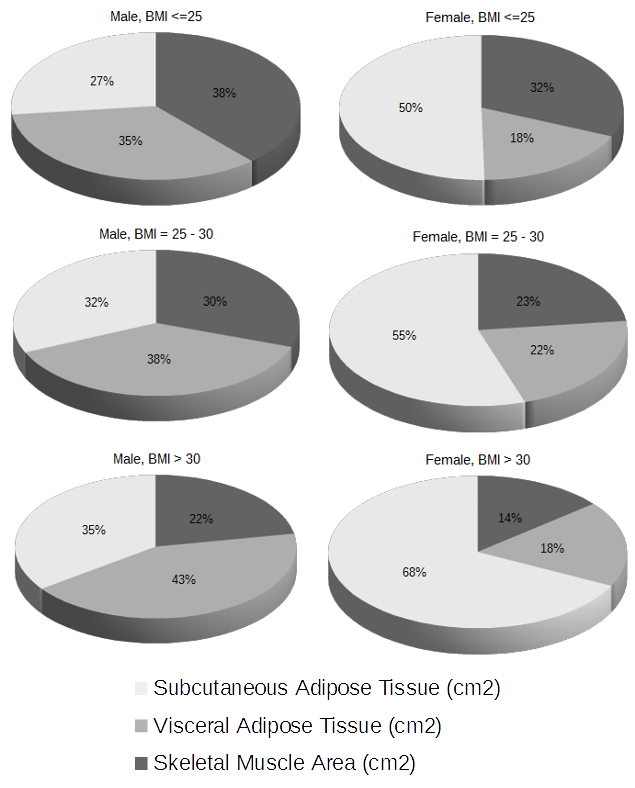
\includegraphics[width=0.8\textwidth]{Figures/bc_gender_bmi_pie}
	\caption{Differences in body composition according to sex and body mass index.}
	\label{fig:bc_gender_bmi}
\end{figure}

The proportion of skeletal muscle area decreases from 38\% in male patients with normal BMI to 22\% in males who are obese. There was a greater decrease in the proportion of skeletal muscle in females with increasing BMI, with skeletal muscle area decreasing from 32\% in females with normal BMI to 14\% in obese females. The higher weight in the high BMI patients was due to a disproportionate increase in adipose tissue rather than skeletal muscle. Moreover, the distribution of the adipose tissue differed between males and females with visceral adipose tissue contributing more to weight in obese males (43\% VAT vs. 35\% SAT) while obese females had a greater proportion of subcutaneous adipose tissue than visceral adipose tissue (18\% VAT vs. 68\% SAT).

\subsection{Correlation with Pulmonary Function Tests}

Partial correlation analysis was performed to study the relationship between pulmonary function tests and body composition. It has been well-established in previous studies that pulmonary function tests are correlated with age and gender and the analysis was therefore adjusted for these two variables. Forced Vital Capacity (FVC, litres), Forced Expiratory Volume in 1 second (FEV1, litres) and the ratio FEV1/FVC (Tiffeneau-Pinelli index,\%) were compared against the various components of body composition. Both FVC and FEV1 were positively correlated with skeletal muscle area but not with adipose tissue area or total cross-sectional area. FEV1/FVC was not correlated with any of the body composition components. 
\todo{move this to discussion}
This would indicate that pulmonary function was dependent on skeletal muscle area while FEV1/FVC, a calculated index to quantify restrictive or obstructive lung disease, was not associated with skeletal muscle area. These results are shown in Table \ref{table:bc_cpet} on page \pageref{table:bc_cpet}.

\subsection{Correlation with Exercise Load}

\begin{figure}[htb]
	\centering
	\begin{subfigure}[b]{0.45\textwidth}
		\centering
		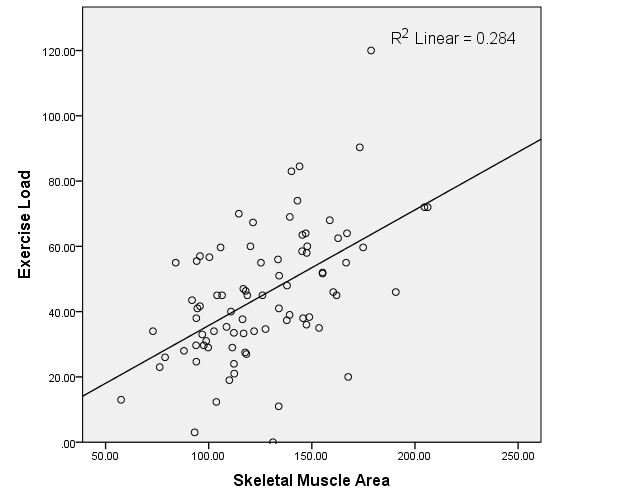
\includegraphics[width=\textwidth]{Figures/bc_scatter_atLoad_skeletal}
		\caption{Anaerobic Threshold}
		\label{fig:bc_at_load_vs_sm}
	\end{subfigure}
	\hfill
	\begin{subfigure}[b]{0.45\textwidth}
		\centering
		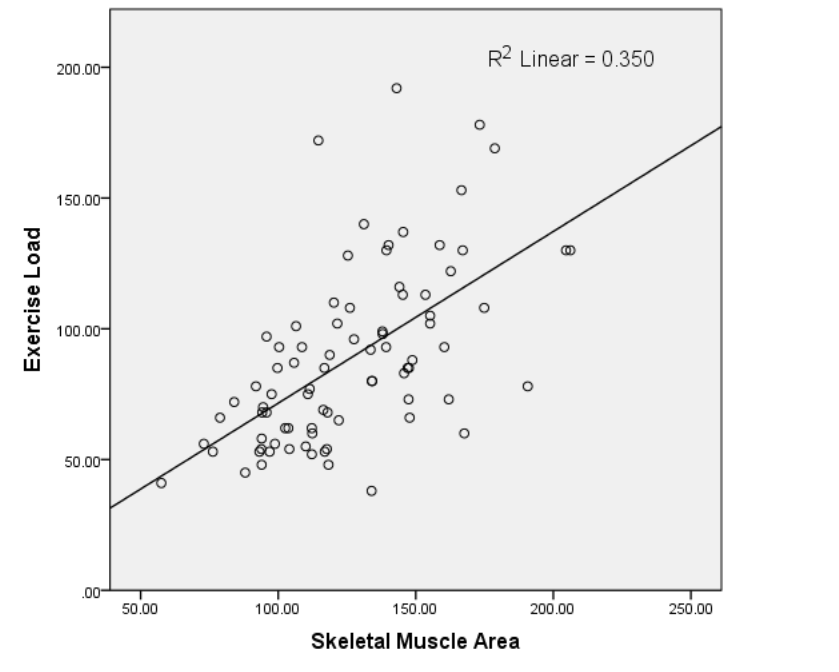
\includegraphics[width=\textwidth]{Figures/bc_scatter_pkLoad_skeletal}
		\caption{Peak Exercise}
		\label{fig:bc_pk_load_vs_sm}
	\end{subfigure}
	\caption{Correlation between exercise load and skeletal muscle area.}	
	\label{fig:bc_load_vs_sm}
	
\end{figure}

Exercise loads achieved at anaerobic threshold and at peak exercise capacity (at volitional stop rather than maximal exercise) were plotted against skeletal muscle area to create scatter-plots(Fig. \ref{fig:bc_load_vs_sm}, p\pageref{fig:bc_load_vs_sm}. Exercise load correlated positively with skeletal muscle area both at anaerobic threshold ($r^{2} = 0.284, p < 0.001$, Fig. \ref{fig:bc_at_load_vs_sm}) and at peak exercise ($r^{2} = 0.350, p < 0.001$, Fig. \ref{fig:bc_pk_load_vs_sm}). However, no correlation was identified between exercise loads achieved and adipose tissue area either at anaerobic threshold ($r^{2} = 0.004, p = 0.587$) or peak exercise ($r^{2} = 0.020, p = 0.206$) as shown in Table \ref{table:bc_cpet} on p\pageref{table:bc_cpet}. 

%This would suggest as one would expect that exercise capacity is mostly related to skeletal muscle volume rather than subcutaneous adipose tissue. - Move this to discussion 

\subsection{Correlation with Oxygen consumption}

%Table 2
\begin{table}[p]
	\caption{The relationship between body composition and cardiopulmonary exercise testing controlled for sex in patients undergoing major pancreatic surgery.}
	\label{table:bc_cpet}
	\footnotesize
	\centering
	\renewcommand{\arraystretch}{1.5} %Increases space between rows
	%\setlength{\tabcolsep}{9pt} %sets the space between columns
	%\hline\noalign{\smallskip} %increases space after the line
	\begin{tabular}{|l| c c | c c | c c | c c|}
		\hline
		                          &  \multicolumn{2}{c|}{Subcut Fat}   & \multicolumn{2}{c|}{Visceral Fat}  &   \multicolumn{2}{c|}{Total Fat}   &    \multicolumn{2}{c|}{Skeletal}     \\
		                          & \multicolumn{2}{c|}{area (cm$^2$)} & \multicolumn{2}{c|}{area (cm$^2$)} & \multicolumn{2}{c|}{area (cm$^2$)} & \multicolumn{2}{c|}{muscle (cm$^2$)} \\
		Variable                  & $\rho$ & p                         & $\rho$ & p                         & $\rho$ & p                         & $\rho$ & p                           \\ \hline
		\multicolumn{9}{|c|}{Pulmonary Function Tests$^a$}                                                                                                                              \\ \hline
		FVC                       & -0.084 & 0.461                     & -0.111 & 0.332                     & -0.112 & 0.325                     & 0.303  & 0.007                       \\
		FEV1                      & -0.050 & 0.659                     & 0.043  & 0.704                     & -0.012 & 0.919                     & 0.350  & 0.002                       \\
		FEV1/FVC                  & 0.0    & 1.0                       & 0.200  & 0.077                     & 0.101  & 0.374                     & 0.003  & 978                         \\ \hline
		\multicolumn{9}{|c|}{At Rest$^b$}                                                                                                                                               \\ \hline
		Minute Ventilation        & 0.117  & 0.303                     & 0.076  & 0.504                     & 0.116  & 0.307                     & 0.136  & 0.230                       \\
		Tidal Volume              & 0.076  & 0.505                     & 0.130  & 0.252                     & 0.116  & 0.305                     & 0.301  & 0.007                       \\
		Absolute $\dot{V}_{O_2}$  & 0.123  & 0.277                     & 0.163  & 0.148                     & 0.164  & 0.145                     & 0.353  & 0.001                       \\
		Corrected $\dot{V}_{O_2}$ & -0.424 & $<$0.001                  & -0.396 & $<$0.001                  & -0.482 & $<$0.001                  & -0.194 & 0.085                       \\
		$O_2$ Pulse               & 0.110  & 0.330                     & 0.134  & 0.238                     & 0.141  & 0.212                     & 0.192  & 0.087                       \\ \hline
		\multicolumn{9}{|c|}{At Anaerobic Threshold$^b$}                                                                                                                                \\ \hline
		Exercise Load             & 0.085  & 0.454                     & 0.085  & 0.454                     & 0.105  & 0.349                     & 0.377  & 0.001                       \\
		Minute Ventilation        & 0.194  & 0.085                     & 0.127  & 0.261                     & 0.198  & 0.076                     & 0.263  & 0.018                       \\
		Tidal Volume              & 0.124  & 0.274                     & 0.154  & 0.172                     & 0.170  & 0.128                     & 0.436  & $<$0.001                    \\
		Absolute $\dot{V}_{O_2}$  & 0.191  & 0.089                     & 0.184  & 0.103                     & 0.231  & 0.038                     & 0.463  & $<$0.001                    \\
		Corrected $\dot{V}_{O_2}$ & -0.326 & 0.003                     & -0.365 & 0.001                     & -0.400 & $<$0.001                  & -0.078 & 0.487                       \\
		$O_2$ Pulse               & 0.181  & 0.108                     & 0.227  & 0.043                     & 0.242  & 0.029                     & 0.338  & 0.002                       \\ \hline
		\multicolumn{9}{|c|}{At Peak Exercise$^b$}                                                                                                                                      \\ \hline
		Exercise Load             & 0.029  & 0.799                     & -0.025 & 0.824                     & 0.020  & 0.859                     & 0.373  & 0.001                       \\
		Minute Ventilation        & 0.080  & 0.483                     & 0.080  & 0.483                     & 0.112  & 0.321                     & 0.242  & 0.029                       \\
		Tidal Volume              & 0.061  & 0.593                     & 0.153  & 0.174                     & 0.138  & 0.219                     & 0.409  & $<$0.001                    \\
		Absolute $\dot{V}_{O_2}$  & 0.087  & 0.444                     & 0.041  & 0.716                     & 0.093  & 0.407                     & 0.375  & 0.001                       \\
		Corrected $\dot{V}_{O_2}$ & -0.295 & 0.008                     & -0.365 & 0.001                     & -0.374 & 0.001                     & -0.027 & 0.813                       \\
		$O_2$ Pulse               & 0.200  & 0.075                     & 0.240  & 0.032                     & 0.261  & 0.019                     & 0.363  & 0.001                       \\ \hline
		\multicolumn{9}{l}{$\rho$ - Pearson's r adjusted for \textit{a} - age and sex and \textit{b} - sex.}
	\end{tabular}
\end{table}

Partial correlations between cardiopulmonary exercise parameters at rest, anaerobic threshold and peak exercise versus body composition were adjusted for gender. Our own findings (\ref{ch_cpet_jaundice}) and the findings of other authors suggest that age is not related to $\dot{V}_{O_2}$AT or $\dot{V}_{O_2}$Peak and therefore no adjustments were made for age. The results of this analysis are shown in Table \ref{table:bc_cpet} (p\pageref{table:bc_cpet}).

Tidal volume ($\dot{V}_T$, litres) was significantly correlated with skeletal muscle area at all phases of exercise including at rest, anaerobic threshold and peak exercise. There was a statistically significant but weak positive correlation between minute ventilation ($\dot{V}_E$, litres) and skeletal muscle at anaerobic threshold and peak exercise but not at rest. There was no correlation between either of these measures of pulmonary function and adipose tissue area at any phase of exercise.

%----------------------------------------------------------------------------------------------
% Correlation between body composition and $\dot{V}_{O_2}$AT before and after correction for total body weight.
\begin{figure}[htb]
	\centering
	\begin{subfigure}[b]{0.45\textwidth}
		\centering
		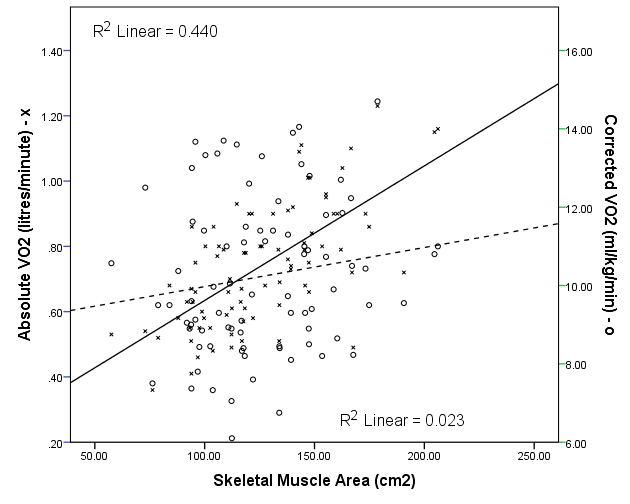
\includegraphics[width=\textwidth]{Figures/bc_scatter_VO2_skeletal}
		\caption{$\dot{V}_{O_2}$AT vs. Skeletal Muscle}
		\label{fig:bc_scatter_VO2_skeletal}
	\end{subfigure}
	\hfill
	\begin{subfigure}[b]{0.45\textwidth}
		\centering
		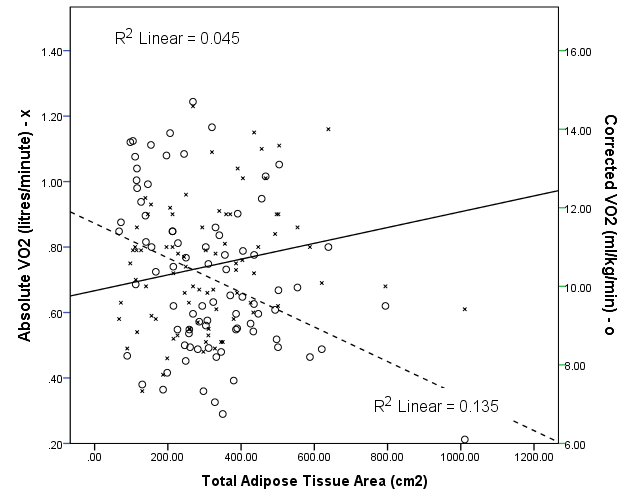
\includegraphics[width=\textwidth]{Figures/bc_scatter_VO2_TAT}
		\caption{$\dot{V}_{O_2}$AT vs. Total Adipose Tissue}
		\label{fig:bc_scatter_VO2_TAT}
	\end{subfigure}
	\caption{Correlation between body composition and $\dot{V}_{O_2}$AT before and after correction for total body weight.}	
	\label{fig:bc_scatter_VO2_bodycomp_reversal}
\end{figure}
%----------------------------------------------------------------------------------------------

Absolute $\dot{V}_{O_2}$ (litres/min) had a strong positive correlation with skeletal muscle area at rest ($\rho = 0.353, p = 0.001$), at anaerobic threshold ($\rho = 0.463, p<0.001$) and at peak exercise ($\rho = 0.375, p = 0.001$). However, this correlation was lost after correction of $\dot{V}_{O_2}$ for total body weight and in fact there was a non-significant change in the direction of correlation to the negative.

Absolute $\dot{V}_{O_2}$ (litres/min) had no correlation with total adipose tissue at rest or at peak exercise and only a weak correlation at anaerobic threshold. However, when it was corrected for total body weight, there was a strong correlation between corrected $\dot{V}_{O_2}$ (mls/kg/min)and total adipose tissue at rest ($\rho = -0.482, p<0.001$), anaerobic threshold ($\rho = -0.400, p<0.001$) and peak exercise ($\rho = -0.374, p = 0.001$).

The loss of the physiological relationship between $\dot{V}_{O_2}$ and skeletal muscle after correcting for total body weight is shown in Fig.\ref{fig:bc_scatter_VO2_skeletal} and the creation of a spurious relationship with total adipose tissue after correction for total body weight is shown in Fig. \ref{fig:bc_scatter_VO2_TAT}.

$O_2$Pulse at the anaerobic thresold and peak exercise was strongly associated with skeletal muscle area with weaker positive correlations with visceral fat and total fat content. There was no correlation between $O_2$Pulse and subcutaneous adipose tissue at any phase of exercise.

%$\dot{V}_{O_2}$ corrected to height seems to correlate best with BC and everything else

\subsection{Scaling $\dot{V}_{O_2}$ to body composition and other factors}


Absolute $\dot{V}_{O_2}$ at the anaerobic threshold was corrected for weight, the square of height, body mass index, skeletal muscle area and estimated lean body mass. Estimated lean body mass (eLBM) was calculated using the Boer formula \parencite{boer_estimated_1984} as shown below.

Men:\ eLBM = 0.407*weight(kg) + 0.267*height(cm) - 19.2

Women:\ eLBM = 0.252*weight(kg) + 0.473*height(cm) - 48.3

The resulting values were compared to body composition, height, weight and body mass index using partial correlations controlling for sex. These results are shown in Table \ref{table:bc_at_new_indices} on p\pageref{table:bc_at_new_indices}. The results from Table \ref{table:bc_cpet} comparing absolute $\dot{V}_{O_2}$ and corrected $\dot{V}_{O_2}$ at the anaerobic threshold with body composition are reproduced in the first two columns of this table to allow comparison with the new indices. $\dot{V}_{O_2}$ scaled for skeletal muscle area had no significant correlation with adipose tissue, height, weight or BMI but had a negative correlation with skeletal muscle area. However, $\dot{V}_{O_2}$ corrected for the square of patient's height had no correlation with adipose tissue but retained a postive correlation with skeletal muscle area. However, there was also a positive correlation with weight and BMI. 

However, when absolute $\dot{V}_{O_2}$ was corrected for lean body mass, there was no correlation with any of the body composition indices or with height, weight or body mass index. The negative correlation that occurs between adipose tissue and $\dot{V}_{O_2}$ corrected for total body weight does not occur when $\dot{V}_{O_2}$ is corrected for lean body mass (Fig. \ref{fig:bc_scatter_VO2_TAT_elbm}). Moreover, the correlation with skeletal muscle area remains unchanged regardless of whether $\dot{V}_{O_2}$ is corrected for total body weight or lean body mass (Fig. \ref{fig:bc_scatter_VO2_skeletal_elbm}).

%----------------------------------------------------------------------------------------------
% Correlation between body composition and $\dot{V}_{O_2}$AT before and after correction for total body weight.
\begin{figure}[htb]
	\centering
	\begin{subfigure}[b]{0.45\textwidth}
		\centering
		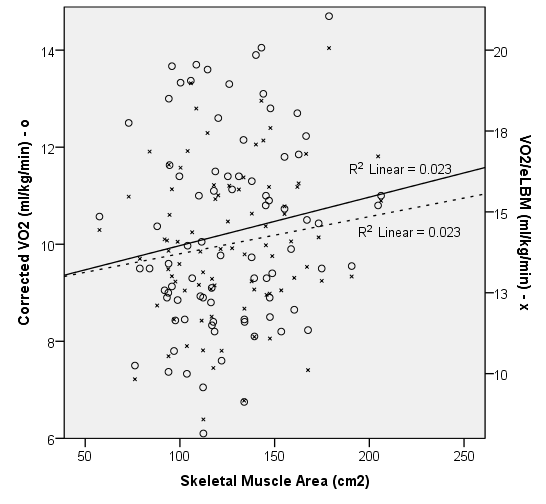
\includegraphics[width=\textwidth]{Figures/bc_scatter_VO2_skeletal_elbm}
		\caption{$\dot{V}_{O_2}$AT vs. Skeletal Muscle}
		\label{fig:bc_scatter_VO2_skeletal_elbm}
	\end{subfigure}
	\hfill
	\begin{subfigure}[b]{0.45\textwidth}
		\centering
		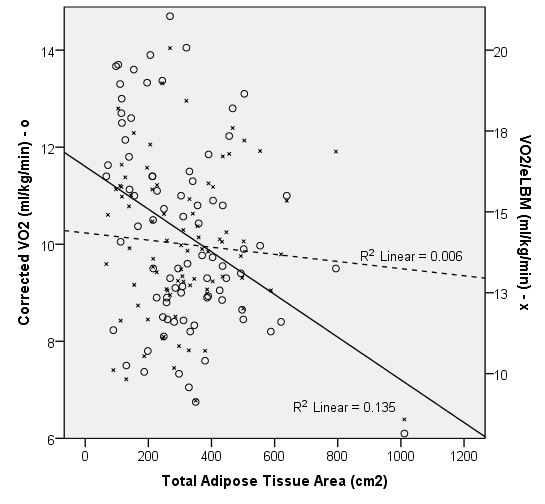
\includegraphics[width=\textwidth]{Figures/bc_scatter_VO2_TAT_elbm}
		\caption{$\dot{V}_{O_2}$AT vs. Total Adipose Tissue}
		\label{fig:bc_scatter_VO2_TAT_elbm}
	\end{subfigure}
	\caption{Correlation between body composition and $\dot{V}_{O_2}$AT corrected for total body weight and estimated lean body mass.}
	\label{fig:bc_scatter_VO2_bodycomp_elbm}
\end{figure}
%----------------------------------------------------------------------------------------------

\begin{sidewaystable}[p]
	\caption{The relationship between body composition, body habitus and $\dot{V}_{O_2}$AT scaled using different factors (controlled for sex) in patients undergoing major pancreatic surgery.}
	\label{table:bc_at_new_indices}
	\footnotesize
	\centering
	\renewcommand{\arraystretch}{1.5} %Increases space between rows
	%\setlength{\tabcolsep}{9pt} %sets the space between columns
	%\hline\noalign{\smallskip} %increases space after the line
	\begin{tabular}{|l|cc|cc|cc|cc|cc|cc|}
		\hline
		& \multicolumn{2}{c|}{Absolute $\dot{V}_{O_2}$} & \multicolumn{2}{c|}{$\frac{\dot{V}_{O_2}}{Weight}$} & \multicolumn{2}{c|}{$\frac{\dot{V}_{O_2}}{Height^2}$} & \multicolumn{2}{c|}{$\frac{\dot{V}_{O_2}}{BMI}$} & \multicolumn{2}{c|}{$\frac{\dot{V}_{O_2}}{Skeletal\ Muscle}$}  & \multicolumn{2}{c|}{$\frac{\dot{V}_{O_2}}{Lean\ Body\ Mass}$}\\
		
		Variable              	& $\rho$ &\textit{p}& $\rho$ &\textit{p}& $\rho$ &\textit{p}& $\rho$ &\textit{p}& $\rho$ &\textit{p}& $\rho$ &\textit{p} \\ \hline
		Subcut. fat (cm$^2$)     & 0.191  &  0.089   & -0.326 &  0.003   & 0.169  &  0.132   & -0.217 &  0.051   & 0.018  &  0.872   & -0.041 & 0.716 \\
		Visceral fat (cm$^2$)    & 0.184  &  0.103   & -0.365 &  0.001   & 0.154  &  0.168   & -0.279 &  0.012   & -0.065 &  0.563   & -0.108 & 0.339\\
		Total fat (cm$^2$)       & 0.231  &  0.038   & -0.400 & $<$0.001 & 0.191  &  0.088   & -0.286 &  0.010   & -0.021 &  0.851   & -0.082 & 0.466\\
		Skeletal Muscle (cm$^2$) & 0.463  & $<$0.001 & -0.078 &  0.487   & 0.329  &  0.003   & 0.105  &  0.353   & -0.429 & $<$0.001 & 0.133 & 0.237 \\
		Height (cm)               & 0.446  & $<$0.001 & 0.019  &  0.870   & 0.001  &  0.993   & 0.475  & $<$0.001 & 0.105  &  0.350   & 0.019 & 0.865\\
		Weight (kg)               & 0.545  & $<$0.001 & -0.302 &  0.006   & 0.358  &  0.001   & -0.043 &  0.703   & 0.001  &  0.995   & 0.033 & 0.770\\
		Body Mass Index (kg/m$^2$)      & 0.357  &  0.001   & -0.363 &  0.001   & 0.425  & $<$0.001 & -0.345 &  0.002   & -0.059 &  0.603   & 0.035 & 0.756\\ \hline
		\multicolumn{11}{l}{$\rho$ - Pearson's partial correlation adjusted for sex.}
	\end{tabular}
	\medskip
	\begin{flushleft}
		$\dot{V}_{O_2}$AT normalised using different measures of body habitus (including weight, square of height, body mass index, skeletal muscle area and estimated lean body mass) was compared to body composition as well as weight, height and BMI in an exploratory analysis. Scaling $\dot{V}_{O_2}$AT using estimated lean body mass was the only method studied that did not result in any 'spurious' correlations with body composition or body habitus. This is also depicted in Fig. \ref{fig:bc_scatter_VO2_bodycomp_elbm} on page \pageref{fig:bc_scatter_VO2_bodycomp_elbm}.
	\end{flushleft}
\end{sidewaystable}




\clearpage

\section{Discussion}

The results of this study demonstrate that the most important cardiopulmonary exercise test parameters used for preoperative risk evaluation in surgery are influenced significantly by the patient's body composition. Both $\dot{V}_{O_2}$AT and $\dot{V}_{O_2}$Peak are significantly affected by patient's body habitus when scaled using total body weight. 
Furthermore, the results suggest that there may be alternate methods of scaling of $\dot{V}_{O_2}$ that removes the effect of body composition on these parameters. 
The results also demonstrate the disproportionate decrease in skeletal muscle area with associated increased in adipose tissue with increasing body mass index. 
Taken together, these results would suggest that caution should be exercised in interpreting $\dot{V}_{O_2}$ (corrected for total body weight, mls/kg/min) in patients with a raised BMI as abnormally low values in these patients may not necessarily be due to poor aerobic fitness or lack of cardiopulmonary reserve. 

\subsection{Oxygen consumption and body composition}

Increased physical activity such as during cardiopulmonary exercise testing results in greater oxygen consumption ($\dot{V}_{O_2}$). The increased demand for oxygen is primarily due to increased metabolic activity within the exercising skeletal muscle.  Therefore, the positive correlation between absolute $\dot{V}_{O_2}$ and skeletal muscle area as has been found here is easily explained by the physiology of aerobic exercise. 

However, current convention is to report $\dot{V}_{O_2}$ measured at cardiopulmonary exercise testing according to the following formula: 
\[Corrected\ \dot{V}_{O_2} (mls.kg^{-1}.min^{-1}) = \frac{Absolute\ \dot{V}_{O_2}\ (litres.min^{-1}) * 1000}{Total\ body\ weight\ (kg)}\]

In chapter \ref{ch_cpet_jaundice}, we reported that there was a significant negative correlation between corrected $\dot{V}_{O_2}$ (ml/kg/min) at the anaerobic threshold as well as at peak exercise and the patient's body mass index in spite of no observable cardiopulmonary comorbid disease (Tables \ref{table:cpet_oj_at_regression} and \ref{table:cpet_oj_peak_regression}). The results of the present study demonstrate that this negative correlation is consequent to the scaling convention used rather than due to any pathophysiological effect of obesity. 

The loss of the strong positive correlation between absolute $VO_{2}$ (litres/min) and skeletal muscle area after correcting for total body weight further supports the argument that the corrected value for $\dot{V}_{O_2}$ under-reports aerobic capacity in obese patients. Moreover, the lack of correlation between pulmonary function tests, tidal volume and minute ventilation and adipose tissue area as well as the slight but statistically significant positive correlation between adipose tissue and $O_2$Pulse at anaerobic threshold as well as peak exercise but not at rest appear to suggest that adiposity did not contribute to poor cardiopulmonary exercise performance in this cohort of patients.

\subsection{Comparison with previous studies}
Our findings are similar to those reported by several authors previously. The relationship between body size, body composition and aerobic capacity both at rest and during exercise has been studied extensively for over a hundred years.

Seltzer reported in his 1940 study of 34 subjects, that individuals who were more `lateral' than `linear' had lower oxygen intakes per kilo body weight.\parencite{seltzer_body_1940} Tanner in his article titled \textit{`Fallacy of per-weight and per-surface area standards, and their relation to spurious correlation'}\parencite{tanner_fallacy_1949} in the Journal of Applied Physiology in 1947 recognised the dangers of expressing physiological variables as a function of total body mass. In a detailed analysis comparing $\dot{V}_{O_2}$ and body build, he concluded that \textit{'as the index wt./stature increases, O2/wt. must be expected to decrease purely as a result of the method used for representing the data.'}

Batterham et al studied 1314 apparently healthy men employed at the National Aeronautics and Space Administration Johnson Space Center in Houston, Texas \parencite{batterham_modeling_1999}. The authors reported that as body mass increased, the proportion composed of fat-free mass decreased. They also found that fat-free mass had a linear relationship with oxygen consumption while total body mass did not. They suggest that ideally estimates of fat-free mass should be used in the representation of oxygen consumption to allow more reliable comparison between subjects. These findings are similar to our results where the proportion of skeletal muscle area decreasing significantly as body mass index increased with a greater decrease in females than males. Moreover, the linear relationship between skeletal muscle area and absolute $\dot{V}_{O_2}$ has also been clearly demonstrated in our findings. 

We used the Boer formula \parencite{boer_estimated_1984}to estimate lean body mass and used this to normalise $\dot{V}_{O_2}$. The resulting value for $\dot{V}_{O_2}$ showed no `spurious' correlations with body composition, height, total body weight or body mass index. These findings are similar to the recommendations made by Janz et al who studied oxygen consumption and aerobic capacity in adolescents over several years as part of the Muscatine study and reported their findings in 1997\parencite{janz_three-year_1997} and 1998 \parencite{janz_longitudinal_1998}. Aerobic capacity in the form of $\dot{V}_{O_2}$peak was evaluated annually in 126 children (mean age 10.3 years) for five years. Body composition changes were also tracked over this period. They reported on the changes in body composition that occur over time and the differences in these changes between circum-pubertal boys and girls. They reported on the significant difficulties in normalising $\dot{V}_{O_2}$ using total body mass and suggested that fat-free mass was the most appropriate variable for normalising $\dot{V}_{O_2}$. They found that $\dot{V}_{O_2}$ normalised using total body mass underestimated aerobic fitness levels of heavier boys and girls. However, this underestimation was greater in girls than in boys. 

Our results demonstrate that there is no correlation between absolute oxygen consumption at rest or during exercise and the amount of adipose tissue. This further emphasises the fact that adipose tissue is metabolically inactive during exercise although it contributes to increased work load. Therefore, dividing absolute $\dot{V}_{O_2}$ by total body weight in overweight/obese subjects whose extra weight is largely due to adipose tissue results in lower corrected $\dot{V}_{O_2}$ as we have demonstrated here. 
Goran et al reported that total body fat did not affect maximal aerobic capacity \parencite{goran_total_2000}. They reported on $\dot{V}_{O_2}$max in obese women before and after weight loss. $\dot{V}_{O_2}$max corrected for total body weight was significantly lower in the obese state while $\dot{V}_{O_2}$max corrected for fat-free mass did not change significantly after weight loss. They also reported that the limiting factor in the obese state was not the cardio-respiratory system but the fact that it was more difficult for obese individuals to do the same amount of work as a normal weight person in weight-bearing activities. This is likely due to the extra fat mass in these individuals that did not contribute to aerobic capacity but instead may increase the exercise load.

These findings have been replicated by several other authors in different subject groups \parencite{loftin_scaling_2001,  lemaitre_maximum_2006,savonen_current_2012, krachler_cardiopulmonary_2014}. Several of the above studies also recommended using allometric scaling to avoid the confounding effects of total body weight. However, this has not gained widespread clinical use.

In a study aimed at determining the optimal method of expressing $\dot{V}_{O_2}$max, Maciejczyk and coworkers analysed the differing influence of body fat and lean body mass on aerobic performance in two groups of physically fit men categorised based on their body fat percentage \parencite{maciejczyk_influence_2014}. They reported that high body mass regardless of composition was correlated negatively with $\dot{V}_{O_2}$ when it was corrected for total body weight penalising otherwise fit men purely based on the proportion of body weight that was contributed by body fat. However, when $\dot{V}_{O_2}$ was corrected for lean body mass, they found that the results were similar between the low body fat and high fat body groups. They, similar to Goran et al\parencite{goran_total_2000}, recommend that $\dot{V}_{O_2}$ be normalised to lean body mass rather than total body weight.

The conclusion from the above studies would be that oxygen consumption normalised for total body weight unfairly penalises obese patients in the absence of true impairment of cardio-respiratory function. This has significant clinical implications as outlined below.

\subsection{Clinical implications of spurious correlation}

The term \textit{`spurious correlation'} was first introduced by English mathematician and biometrician, Karl Pearson in 1896. He used the term to describe correlations that occurred as a result of using ratios instead of absolute values rather than because of any actual correlations between the variables being studied \parencite{pearson_mathematical_1896}.

Older et al in their pioneering study in 1993 reported that $\dot{V}_{O_2}$AT < 11mls/kg/min was associated with increased mortality in elderly patients undergoing major abdominal surgery \parencite{older_preoperative_1993}. While they did not provide any data on other preoperative or intra-operative factors, they concluded that cardiopulmonary exercise testing was useful in predicting postoperative outcome. However, this first report on the use of cardiopulmonary exercise testing as a preoperative risk assessment tool concluded that a $\dot{V}_{O_2}$AT < 11mls/kg/min represented cardiac failure. This association is repeated in their later work on 548 patients which also showed a clear association between $\dot{V}_{O_2}$AT < 11mls/kg/min and mortality due to cardiovascular causes \parencite{older_cardiopulmonary_1999}. The concepts of \textit{'surgical anaerobic threshold'} and \textit{'postoperative cardiac failure'} were introduced later and were described as the \textit{'inability of the heart to meet the demand of postoperative stress.'}\parencite{society_ats/accp_2003}.

Swart and Carlisle reported that $\dot{V}_{O_2}$AT < 11mls/kg/min in patients undergoing open colorectal surgery was associated with adverse outcomes \parencite{swart_case-controlled_2012}. However, the proportion of females in the low $\dot{V}_{O_2}$AT group was significantly greater than that in the normal $\dot{V}_{O_2}$AT groups (24\% vs 51\%). The average corrected $\dot{V}_{O_2}$AT in men calculated from the data presented in their paper was 11.02 mls/kg/min while in women it was 9.81 mls/kg/min. In a study by Wilson et al that reported cardiopulmonary exercise testing predicted outcome in major elective intra-abdominal surgery, the proportion of females in the low $\dot{V}_{O_2}$AT group was 51\% while it was 28\% in the group with normal AT \parencite{wilson_impaired_2010}. There was no data presented on body mass index in this study. We reported in Chapter \ref{ch_cpet_jaundice} that females were more likely to have a lower $\dot{V}_{O_2}$AT (Table \ref{table:cpet_oj_at_regression}) and lower $\dot{V}_{O_2}$Peak (Table \ref{table:cpet_oj_peak_regression}). However, all the results in the present study were controlled for the effect of sex. 

The `obesity paradox' would suggest that, in fact, obese patients are not necessarily at an increased risk of postoperative complications. Several authors have reported that obesity is not a risk factor for major complications after pancreaticoduodenectomy \parencite{khan_does_2010, tsai_impact_2010, balentine_obesity_2011}. 
In a large study of 118,707 patients undergoing non-bariatric general surgery, the authors reported that the risk of death was `paradoxically' low in the overweight and obese group of patients \parencite{mullen_obesity_2009}. The results of the present study show that $\dot{V}_{O_2}$ as is currently reported for clinical use will also be low in this very same cohort of patients. 
This obesity paradox is particularly apparent in patients with heart failure where in spite of a low $\dot{V}_{O_2}$ (corrected for total body weight), obese patients have better survival rates. Horwich and co-workers reported in a study of 2331 patients that body mass index was associated with a low $\dot{V}_{O_2}$Peak (ml/kg/min) independent of all other factors including age, diabetes, cardiac disease, New York Heart Association Class of cardiac failure and race \parencite{horwich_relationship_2009}.

It is clear from the review presented in Chapter \ref{ch_intro} as well as the results presented in Chapter \ref{ch_cpet_outcomes}, that cardiopulmonary exercise testing is useful in predicting risk after major surgery. Cardiopulmonary exercise testing has become ubiquitous in the preoperative assessment of complex surgical patients. However, the present study demonstrates that cardiopulmonary exercise test parameters in the overweight/obese patient must be interpreted with caution, especially when used to select patients who may be declined surgery based on these results. 

\subsection{Measuring impact of prehabilitation}

Where time to surgery is not critical, prehabilitation has gained an increasingly important role in optimising patients for surgery, reducing complications \parencite{jones_effects_2007, dronkers_preoperative_2010, valkenet_effects_2010, gillis_prehabilitation_2014} and mitigating the effects of neoadjuvant oncological therapy\parencite{west_effect_2015}.
Cardiopulmonary exercise testing has been reported to be a useful objective measure of the impact of prehabilitation in surgical patients \parencite{west_effect_2015}.

The success of such prehabilitation programs must not be determined solely by $\dot{V}_{O_2}$ corrected for total body weight. Instead, improvement in the absolute values of $\dot{V}_{O_2}$AT and $\dot{V}_{O_2}$Peak in conjunction with improvement in other parameters that are not affected by body composition such as $O^2$Pulse, tidal volume\parencite{jones_effects_2007} or maximal exercise load may provide more reliable evidence of improvement in aerobic capacity. The combination of nutritional assessment and advice, home-based exercise programs and weight loss will help improve aerobic capacity and eventually postoperative outcomes. 

Further studies are required to validate the findings presented here as well as to identify optimal scaling methods for cardiopulmonary exercise test parameters. This will improve the clinical utility of cardiopulmonary exercise testing in the preoperative risk assessment as well as optimisation of patients undergoing major surgery.

%This needs to be expanded significantly. 

%Mention studies that have used VE/VCO2. 
%I think there is a study in bariatrics where bmi and at were independent predictors. 
%Mention studies that used predicted VO2 or absolute $\dot{V}_{O_2}$ where calculated AT was not useful. 
%This should give me at least another 2 paragraphs














%% Chapter 05 - CPET, complications and survival

\chapter{An investigation into the relationship between cardiopulmonary exercise testing, comorbidity, systemic inflammation and survival after pancreaticoduodenectomy for cancer.}
\label{ch_survival}

\lhead{Chapter \ref{ch_survival}. \emph{CPET, Complications and Survival}} % This is for the header on each page - perhaps a shortened title

\clearpage
%----------------------------------------------------------------------------------------

\section{Introduction}
Median survival after pancreaticoduodenectomy for pancreatic ductal adenocarcinoma varies from approximately 18 months to 24 months.\parencite{winter_1423_2006,neoptolemos_adjuvant_2010} 

Selecting patients who will benefit from the survival advantage that a pancreaticoduodnectomy offers is important to maximise the usefulness of this morbid procedure.

Comorbidity is not only associated with postoperative morbidity and mortality (Section \ref{sec:comorbidity_risk_stratification}) but has also been reported to be associated with poor long-term survival in patients undergoing surgery several different cancers including colorectal cancer \parencite{} and breast cancer.\parencite{} With 10-year survival rates approaching 60\% and 80\% in these patients, it is not surprising that some patients with significant comorbidity may die from their comorbid disease rather than from cancer recurrence. However, cancer-specific survival is also shorter in patients with significant comorbidities.

Systemic inflammation has been proposed as one of the intermediary mechanism in these patients that increases rates of recurrence and decreases disease free survival. The modified Glasgow Prognostic Score, a measure of preoperative systemic inflammation in cancer patients, is associated with poor survival regardless of the site or stage of cancer. This is discussed in detail in Section \ref{sec:intro_systemic_inflammation_outcome}. 

However, an objective method to measure comorbidity itself remains elusive and various scores have been used for this purpose. The Charlson Comorbidity Index is one such score and has been reported to predict long-term survival in cancer patients. Cardiopulmonary exercise testing is an objective measure of aerobic fitness and of cardiorespiratory comorbidity and has been shown to be useful in predicting complications after major abdominal surgery including pancreatic surgery. (\parencite{ausania_effects_2012} and Chapter \ref{ch_cpet_outcomes})

Moreover, cardiopulmonary exercise testing has been used to predict medium term survival after aortic aneurysm surgery \parencite{carlisle_mid-term_2007} as well as overall survival in patients with medical diseases such as chronic heart failure or chronic obstructive airways disease. The relationship between cardiopulmonary exercise testing and long-term survival in patients undergoing pancreaticoduodenectomy for cancer has not been reported before. 

\section{Aim}
The aim of the present study was to investigate the relationship between cardiopulmonary exercise testing, comorbidity, systemic inflammation and survival in patients undergoing pancreaticoduodenectomy for pancreatic ductal adenocarcinoma.

\section{Patients and Methods}
All patients who underwent pancreaticoduodenectomy for pancreatic ductal adenocarcinoma between August 2008 and July 2012 were included in the study. Data was collected prospectively in a structured database and included demographics, preoperative clinico-pathological characteristics, cardiopulmonary exercise testing, postoperative complications, tumour characteristics and long-term survival. Survival data was collected using the Greater Glasgow and Clyde NHS Clinical Portal and the Scottish National Statutory Register of Deaths. The modified Glasgow Prognostic Score was calculated as described in Table \ref{table:mGPS} on p\pageref{table:mGPS}. The POSSUM Physiology Score was calculated as described in \ref{}. 

The Scottish Index of Multiple Deprivation (SMID) combines 38 indicators across 7 domains including  income, employment, health, education, skills and training, housing, geographic access and crime.  All of Scotland's population is placed into 6505 geographical groups ranked in descending order of deprivation. SMID quintiles place these into 5 categories with 1 representing the most deprived areas and 5 representing the least deprived. The SMID quintile for each patient was derived from the postcode of their primary residence.

\subsection{Statistics}
Standard thresholds were used to categorise continuous variables where applicable. Kaplan-Meir survival analysis and Cox-regression analysis were used to study the relationship between preoperative clinico-pathological characteristics and long-term survival. SPSS version 22 statistical software package was used for all analysis.



\section{Results}


\section{Discussion}

 This is considerably less than other common cancers such as colorectal cancer or breast cancer where 5-year survivals across all stages are 60\% and 90\% respectively. However, only 10-20\% of pancreatic cancers are suitable for potentially curative surgery and of patients who undergo curative surgery 5-year survival remains low at approximately 20\%.\parencite{cancerresearchuk_cancer_2014}
% Chapter 06 - Postop CRP and complications

\chapter{An investigation into the relationship between postoperative systemic inflammation and complications after pancreaticoduodenectomy.}
\label{ch_crp_comp}

\lhead{Chapter \ref{ch_crp_comp}. \emph{Postoperative CRP and complications}} % This is for the header on each page - perhaps a shortened title

\clearpage
%----------------------------------------------------------------------------------------
\section{Introduction}
Pancreaticoduodenectomy is associated with significant morbidity in spite of advances in patient selection, perioperative care and surgical technique. Early identification of complications can help improve outcomes by better allocation of critical care resources as well as goal-directed therapy. Postoperative pancreatic fistula is one of the most dreaded complications after a pancreaticoduodenectomy and can lead to a cascade of other complications including delayed haemorrhage, infected intra-abdominal collections, delayed gastric emptying, prolonged hospitalisation and in some cases, death. The International Study Group for Pancreatic Fistula (ISGPF) have not only defined what constitutes a post-operative pancreatic fistula but have also graded the severity of this complication based on its impact on the management of the patient. However, these definitions are applied after the event and there is no clear way of predicting the severity of complications.

Postoperative CRP levels have been shown to predict infective complications after major surgery including colorectal,  oesophago-gastric and pancreatic surgery. \parencite{mustard_c-reactive_1987, matthiessen_increase_2008, mcneer_early_2010, dutta_persistent_2011, mackay_c-reactive_2011, murakami_soft_2008, welsch_persisting_2008} It has been postulated that an unmitigated and exaggerated systemic inflammatory response in the early postoperative period is followed by a compensatory anti-inflammatory response that predisposes the patient to sepsis and impaired healing. 

But, the mechanisms underlying the pathogenesis of post-operative pancreatic fistula are largely attributed to anatomical factors including soft texture of the pancreas and small pancreatic duct diameter as well as surgical technique with increased intra-operative blood loss and pancreatico-jejunostomy rather than pancreatico-gastrostomy being associated with increased incidence of anastomotic leakage. The association between the early postoperative systemic inflammatory response and the incidence and severity of postoperative pancreatic fistula has not been reported. Moreover, the role postoperative CRP in predicting infective complications when these occur in association with postoperative pancreatic fistula has not been studied either. 

The aim of this study was to investigate the association between systemic inflammation, postoperative pancreatic fistula and infective complications in patients undergoing pancreaticoduodenectomy.

\section{Methods}
\todo{Check dates for this study}
Patients who underwent elective pancreaticoduodenectomy between January 2008 and July 2012 were included in this study. Patients who underwent only a trial dissection or trial dissection and surgical bypass during this period were excluded. All patients were given antibiotic prophylaxis at induction and this was continued for 24 hours after surgery. All patients had general anaesthesia supplemented either with patient-controlled epidural analgesia or spinal diamorphine and patient-controlled opiate analgesia for postoperative pain relief. Octreotide (200$\mu$g) was administered subcutaneously three times a day for 5 days in all patients and continued longer in patients diagnosed with a postoperative pancreatic fistula. Patients were routinely admitted to the surgical high dependency unit where a standardised regimen was followed for early mobilisation, chest physiotherapy and early enteral nutrition. All patients had one or two surgical drain(s) placed at the time of surgery which were removed at the clinician's discretion during the postoperative period based on the presence or absence of postoperative pancreatic fistula or other intra-abdominal collections. 

Patients had routine measurements of inflammatory markers including C-reactive protein (CRP) and differential white cell counts from the day before surgery and every day for at least a week after surgery. These results including the preoperative blood tests and the postoperative blood tests for the first 7 days after surgery were collected from the hospital laboratory databases.

All complications were discussed at a weekly morbidity meeting and prospectively recorded in an electronic database.  The diagnosis and grading of pancreas-specific complications including postoperative pancreatic fistula (POPF, Section \ref{sec:ch_intro_POPF}) and post-pancreatectomy haemorrhage (PPH, Section \ref{sec:ch_intro_PPH}) were made according to the International Study Group classifications as shown in Table \ref{table:isgps_popf} and Table \ref{table:isgps_pph} on p\pageref{table:isgps_popf} respectively.

All other complications were graded using the Clavien-Dindo classification system as shown in Table \ref{table:clavien-dindo}. This allowed the grading of the severity of the complications based on the magnitude of the intervention(s) required to treat them. Postoperative mortality was defined as death within 30-days of the operation or while still in hospital after the operation. Re-intervention in the form of radiological, endoscopic or surgical procedures was recorded prospectively.

\subsection{Statistics}
Mann-Whitney U test was used to compare the distribution of postoperative CRP (as a continuous variable) in patients who had a complication and those who did not. Data are presented as median (inter-quartile range, IQR) unless otherwise specified. Line plots with error bars depicting 95\% confidence intervals are used to depict the trends in CRP over time across different patient groups. 

Receiver operating characteristic (ROC) analysis \parencite{robertson_use_1981,zweig_receiver-operating_1993} was used to identify the optimum thresholds for postoperative CRP for predicting infective complications with a preference for thresholds that had a greater negative predictive value. Patients were categorised using these thresholds to analyse the relationship between CRP (as a categorical variable) and re-operation, hospital stay, critical care stay, number of critical care admissions as well as postoperative mortality using the Chi-square test. 

SPSS software (Version 22.0; IBM, USA) was used to perform statistical analysis. Effects were considered significant at $\alpha \leq0.05$. 

\todo{Complete this section - most of this can be modified from the stats sections in other chapters}


\section{Results}
\subsection{POPF, infective complications and other outcomes}
Pancreaticoduodenectomy was performed in 188 patients (126 male, 67\%) during the study period. The median age was 63.5 years (IQR 54 - 70 years). 79 (42\%) patients were over the age of 65 years. 

Post-operative pancreatic fistula (POPF) as defined by the International Study Group for Pancreatic Fistula (ISGPF) occurred in 62 (33\%) patients. Of these patients, 19 (10.1\%) had a Grade A POPF, 25 (13.3\%) had a Grade B POPF and 18 (9.6\%) had a Grade C POPF. Significant infective complications of Clavien-Dindo grade 3 or higher occurred in 84 patients. Infectious complications were more common in patients with age $>$65 years (35.6\% vs. 50.0\%, p=0.046) and $\dot{V}_{O_2}$AT$<$10 ml/kg/min (28.8\% vs. 52.4\%, p=0.006) were significantly associated with infective complications. Gender, body mass index, smoking status, modified Glasgow Prognostic Score, preoperative serum bilirubin and POSSUM physiology score were not associated with infective complications.

Infectious complications were also significantly associated with other complications including post-operative pancreatic fistula, post-pancreatectomy haemorrhage, length of stay in hospital, critical care stay, number of critical care admissions, re-operation rates and in-hospital mortality. (Table \ref{table:crp_comp_infect_vs_other_complications})

%12/07/15 - Started this table
\begin{table}[p]
	\centering
	\caption{The relationship between preoperative clinicopathological characteristics and infective complications in patients undergoing pancreaticoduodenectomy.}
	\label{table:crp_comp_preop_factors}
	\renewcommand{\arraystretch}{1.5} %Increases space between rows
	\setlength{\tabcolsep}{12pt} %sets the space between columns
	\begin{tabular}{|l l c c c|}
		\hline
		                  &          & \multicolumn{2}{c}{Infective complication} &  \\
		                  &          & CD 0 - 2    & CD 3 - 5                       & p     \\ \hline
		Age               & $\leq$65 & 67 (64.4\%) & 42 (50.0\%)                    & 0.046 \\
		                  & $>$65    & 37 (35.6\%) & 42 (50.0\%)                    &  \\
		Gender            & Male     & 70 (67.3\%) & 56 (66.7\% )                   & 0.926 \\
		                  & Female   & 34 (32.7\%) & 28 (33.3\%)                    &  \\
		BMI               & $\leq$25 & 48 (50.5\%) & 37 (46.3\%)                    & 0.573 \\
		                  & $>$25    & 47 (49.5\%) & 43 (53.8\%)                    &  \\
		Smoking           & No       & 53 (62.4\%) & 44 (59.5\%)                    & 0.709 \\
		                  & Yes      & 32 (37.6\%) & 30 (40.5\%)                    &  \\
		mGPS              & 0        & 67 (64.4\%) & 49 (59.8\%)                    & 0.570 \\
		                  & 1        & 7 (6.7\%)   & 9 (11.0\%)                     &  \\
		                  & 2        & 30 (28.8\%) & 24 (29.3\%)                    &  \\
		Bilirubin         & $\leq$35 & 66 (63.5\%) & 47 (56.0\%)                    & 0.574 \\
		                  & 35 - 250 & 22 (21.2\%) & 22 (26.2\%)                    &  \\
		                  & $>$250   & 16 (15.4\%) & 15 (17.9\%)                    &  \\
		$\dot{V}_{O_2}$AT & $\geq$10 & 47 (71.2\%) & 30 (47.6\%)                    & 0.006 \\
		                  & $<$10    & 19(28.8\%)  & 33 (52.4\%)                    &  \\
		PPS               & $\leq$14 & 56 (56.0\%) & 37 (46.3\%)                    & 0.193 \\
		                  & $>$14    & 44 (44.0\%) & 43 (53.8\%)                    &  \\ \hline
		\multicolumn{5}{l}{CD - Clavien-Dindo Grade, BMI - Body Mass Index}                 \\
		\multicolumn{5}{l}{mGPS - Modified Glasgow Prognostic Score}       \\
		\multicolumn{5}{l}{PPS - POSSUM Physiology Score}                                   \\
		\multicolumn{5}{l}{p - Chi-square test}
	\end{tabular}
\end{table}


		
		
		

%12/07/15 - Started this table
\begin{table}[p]
	\centering
	\caption{The relationship between infective complications and other adverse events in patients undergoing pancreaticoduodenectomy.}
	\label{table:crp_comp_infect_vs_other_complications}
	\renewcommand{\arraystretch}{1.2} %Increases space between rows
	\setlength{\tabcolsep}{9pt} %sets the space between columns
	\begin{tabular}{|l l | c c |c|}
		\hline
		                         &               & \multicolumn{2}{c|}{Infective complication} & \\
		                         &               & CD 0 - 2     & CD 3 - 5     & p              \\ \hline
		POPF                     & No            & 85 (81.7\%)  & 41 (48.8\%)  & $<$0.001       \\
		                         & Grade A       & 10 (9.6\%)   & 9 (10.7\%)   &  \\
		                         & Grade B       & 7 (6.7\%)    & 18 (21.4\%)  &  \\
		                         & Grade C       & 2 (1.9\%)    & 16 (19.0\%)  &  \\
		PPH                      & No            & 95 (92.2\%)  & 64 (77.1\% ) & 0.048          \\
		                         & Grade A       & 2 (1.9\%)    & 2 (2.4\%)    &  \\
		                         & Grade B       & 2 (1.9\%)    & 6 (7.2\%)    &  \\
		                         & Grade C       & 4  (3.9\%)   & 11 (13.2\%)  &  \\
		Postop Stay              & $\leq$14 days & 65 (62.5\%)  & 17 (20.2\%)  & $<$0.001       \\
		                         & $>$14 days    & 39 (37.5\%)  & 67 (79.8\%)  &  \\
		Critical Care Stay       & $\leq$7 days  & 84 (80.8\%)  & 34 (40.5\%)  & $<$0.001       \\
		                         & $>$7 days     & 20 (19.2\%)  & 50 (59.5\%)  &  \\
		Critical Care admissions & 1             & 92 (88.5\%)  & 53 (63.1\%)  & $<$0.001       \\
		                         & $>$1          & 12 (11.5\%)  & 31 (36.9\%)  &  \\
		Reoperation              & No            & 99 (95.2\%)  & 64 (76.2\%)  & $<$0.001       \\
		                         & Yes           & 5 (4.8\%)    & 20 (23.8\%)  &  \\
		In-hospital mortality    & No            & 103 (99.0\%) & 76 (90.5\%)  & 0.006          \\
		                         & Yes           & 1 (1.0\%)    & 8 (9.5\%)    &  \\ \hline
		\multicolumn{5}{l}{POPF - Post-operative pancreatic fistula}                            \\
		\multicolumn{5}{l}{PPH - Post-pancreatectomy haemorrhage}                               \\
		\multicolumn{5}{l}{p - Chi-square test}
	\end{tabular}
\end{table}


%CRP trends and pancreatic fistula
\subsection{Postoperative CRP and POPF}
Postoperative CRP levels on days 2 through 7 were significantly higher in patients who developed a postoperative pancreatic fistula (p = 0.002 for CRP on Day 2 and p<0.001 for CRP on Days 3 through 7, Mann-Whitney U test). These results are presented in Table \ref{table:crp_comp_vs_POPF_ISGPS_p_values_only} and Fig. \ref{fig:crp_comp_crp_popf} on p\pageref{fig:crp_comp_crp_popf}. Fig. \ref{fig:crp_comp_crp_popf_isgps} shows that CRP in the first postoperative week was not significantly different between postoperative pancreatic fistulae of ISGPF Grade A, B and C. 

However, there is no useful clinical application for the association between CRP in the early postoperative period and  pancreatic fistula as the diagnosis of POPF is based on the the amylase content in surgical drains on the third postoperative day. Moreover, early postoperative CRP did not predict the severity of the pancreatic fistula either.

%========================CRP vs POPF============================================
%CRP trends in a 2-panel figure and table showing p-values below it
\clearpage
\begin{figure}[t]
	\caption{Serum CRP levels in the first week after pancreaticoduodenectomy in patients with postoperative pancreatic fistula (POPF).}
	\label{fig:crp_comp_crp_popf}
	\centering
	\begin{subfigure}{0.48\textwidth}
		\centering
		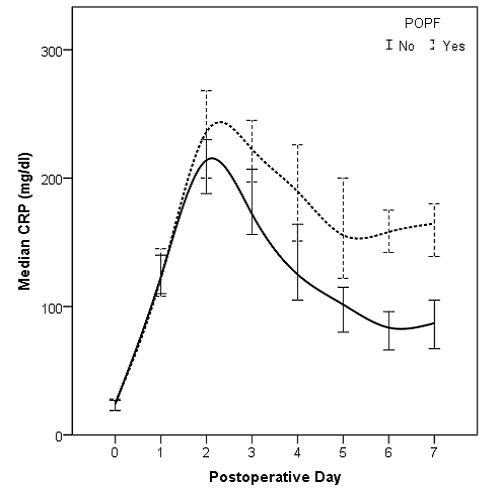
\includegraphics[width=\textwidth]{Figures/crp_comp_crp_popf_yes_no}
		\caption{POPF Absent vs. Any Grade}
		\label{fig:crp_comp_crp_popf_yes_no}
	\end{subfigure}
	\hfill
	\begin{subfigure}{0.48\textwidth}
		\centering
		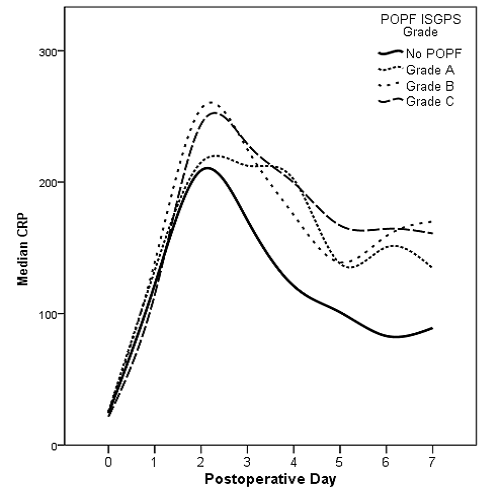
\includegraphics[width=\textwidth]{Figures/crp_comp_crp_popf_isgps}
		\caption{POPF ISGPF Grades}
		\label{fig:crp_comp_crp_popf_isgps}
	\end{subfigure}
\end{figure}
\hfill
%06/07/15 - Started this table
\begin{table}[h]
	\centering
	\caption{The relationship between CRP during the first postoperative week and post-operative pancreatic fistula (POPF) in patients undergoing pancreaticoduodenectomy.}
	\label{table:crp_comp_vs_POPF_ISGPS_p_values_only}
	\renewcommand{\arraystretch}{1.2} %Increases space between rows
	%\setlength{\tabcolsep}{9pt} %sets the space between columns
	\begin{tabular}{| c | c c c c |}
		\hline
		           &       \multicolumn{4}{c|}{POPF ISGPS Grades - \textit{p}}        \\
		Postop Day & No vs. Any Grade & No vs. A & A vs. B & B vs. C                 \\ \hline
		0          & 0.722            & 0.582    & 0.849   & 0.730                   \\
		1          & 0.242            & 0.331    & 0.740   & 0.295                   \\
		2          & 0.002            & 0.161    & 0.222   & 0.563                   \\
		3          & $<$0.001         & 0.022    & 0.602   & 0.530                   \\
		4          & $<$0.001         & 0.007    & 0.906   & 0.834                   \\
		5          & $<$0.001         & 0.035    & 0.611   & 0.959                   \\
		6          & $<$0.001         & 0.012    & 0.638   & 0.781                   \\
		7          & $<$0.001         & 0.006    & 0.235   & 0.356                   \\ \hline
		\multicolumn{5}{l}{\textit{p} - Mann-Whitney U test}                         \\
		\multicolumn{5}{l}{ISGPS - International Study Group for Pancreatic Surgery}	\\
				\multicolumn{5}{l}{POPF - Postoperative Pancreatic Fistula}
	\end{tabular}
	
	
\end{table}
%==============================================================================
\clearpage

\subsection{Postoperative CRP and infective complications}
The median CRP levels on or after postoperative day 3 were significantly higher in patients who developed clinically significant infective complications in the absence of a POPF (Fig. \ref{fig:crp_comp_infective_leak0}). Moreover, the median difference in CRP also increases from 56 mg/L on the third day to 79 mg/L on the seventh day. However, there was no such association in patients who did develop a POPF (Fig. \ref{fig:crp_comp_infective_leak1}).  For instance, difference in median CRP on Day 4 in patients who did not develop a POPF and did not have an infective complication was 97 mg/L (IQR 71 - 174) but was 173 mg/L if they had an infective complication. (p$<$0.001). However, in patients who had POPF, the CRP on day 4 was 214 mg/L (IQR 151 - 250) in the absence of infective complications and 190 mg/L (IQR 137 - 252) in the presence of infective complications. (p = 0.559)

Therefore, CRP on or after the third postoperative day appears to be useful in predicting infective complications only in patients who did not develop a POPF and these results are shown in Table \ref{table:crp_comp_vs_infections_popf_y1n0} and Fig. \ref{fig:crp_comp_infective_leak} on p\pageref{fig:crp_comp_infective_leak}. 

%========================CRP vs Infections====================================
%CRP trends vs infections in patients with or without popf in a 2-panel figure and table showing median, iqr and p-values below it
\clearpage
\begin{figure}[t]
	\caption{Relationship between postoperative CRP and clinically significant infective complications in patients without (A) and with (B) POPF.}
	\label{fig:crp_comp_infective_leak}
	\centering
	\begin{subfigure}{0.48\textwidth}
		\centering
		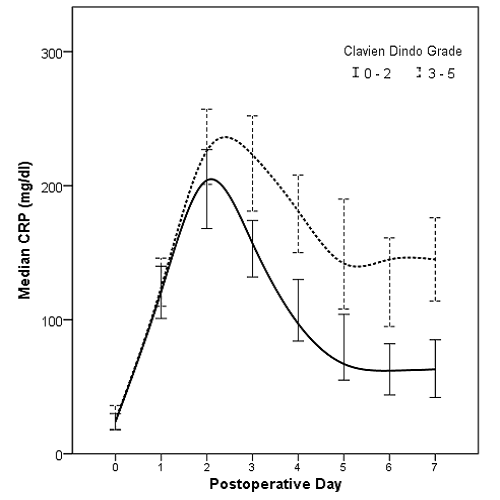
\includegraphics[width=\textwidth]{Figures/crp_comp_infective_leak0}
		\caption{Patients with \textbf{\underline{no}} POPF}
		\label{fig:crp_comp_infective_leak0}
	\end{subfigure}
	\hfill
	\begin{subfigure}{0.48\textwidth}
		\centering
		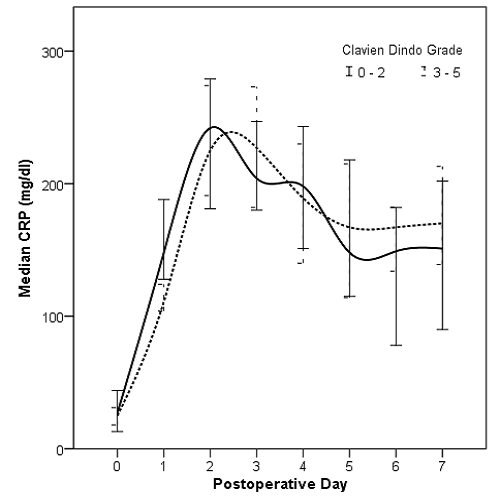
\includegraphics[width=\textwidth]{Figures/crp_comp_infective_leak1}
		\caption{Patients with POPF}
		\label{fig:crp_comp_infective_leak1}
	\end{subfigure}
\end{figure}
\vfill
%07/07/15 - Started this table
\begin{table}[h]
	\centering
	\caption{The relationship between postoperative CRP and infectious complications grouped by POPF. (Mann-Whitney U test)}
	\label{table:crp_comp_vs_infections_popf_y1n0}
	%\renewcommand{\arraystretch}{1.1} %Increases space between rows
	%\setlength{\tabcolsep}{9pt} %sets the space between columns
	\begin{tabular}{| c | c c c | c c c |}
		\hline
		           &       \multicolumn{3}{c}{POPF Absent}       &      \multicolumn{3}{c}{POPF Present}       \\
		           & \multicolumn{3}{c}{Infectious Complication} & \multicolumn{3}{c}{Infectious Complication} \\
		Postop Day & No          & Yes         & p               & No          & Yes         & p               \\
		           & (n=85)      & (n=41)      &                 & (n=19)      & (n=43)      &  \\ \hline
		0          & 24          & 25          & 0.379           & 27          & 25          & 0.629           \\
		           & (12 - 42)   & (14 - 41)   &                 & (13 - 44)   & (16 - 34)   &  \\
		1          & 122         & 123         & 0.667           & 148         & 116         & 0.038           \\
		           & (85 - 156)  & (87 - 148)  &                 & (114 - )    & (94 - 161)  &  \\
		2          & 204         & 218         & 0.203           & 242         & 228         & 0.919           \\
		           & (136 - 242) & (165 - 262) &                 & (181 - 279) & (186 - 296) &  \\
		3          & 157         & 213         & 0.011           & 206         & 226         & 0.846           \\
		           & (105 - 211) & (150 - 258) &                 & (180 - 297) & (175 - 281) &  \\
		4          & 97          & 173         & $<$0.001        & 214         & 190         & 0.559           \\
		           & (71 - 174)  & (118 - 216) &                 & (151 - 250) & (137 - 252) &  \\
		5          & 76          & 122         & $<$0.001        & 140         & 167         & 0.639           \\
		           & (40 - 129)  & (87 - 202)  &                 & (115 - 218) & (111 - 222) &  \\
		6          & 64          & 121         & $<$0.001        & 148         & 168         & 0.275           \\
		           & (31 - 133)  & (87 - 172)  &                 & (78 - 182)  & (109 - 224) &  \\
		7          & 62          & 141         & $<$0.001        & 158         & 167         & 0.644           \\
		           & (25 - 106)  & (90 - 190)  &                 & (90 - 231)  & (101 - 226) &  \\ \hline
		\multicolumn{7}{l}{Values are median (inter-quartile range.)}                                          \\
		\multicolumn{7}{l}{p - Mann-Whitney U test)}
	\end{tabular}
\end{table}
%==============================================================================
\clearpage

\subsection{Postoperative white cell counts, albumin and infective complications}

Patients who developed infective complications in the absence of POPF had a raised total white cell counts on postoperative days 5, 6 and 7 which were statistically significant However, these differences were small with wide, overlapping 95\% confidence intervals (Fig. \ref{fig:crp_comp_WCC_infective_leak0}) and not clinically significant. For instance, the median white cell count on the fifth postoperative day in patients who did not have an infective complication was 8.9 (IQR 6.6 - 11) while in patients who had an infective complication it was 9.8 (IQR 7.9 - 13). While this difference was statistically significant (p = 0.028), both medians were within the normal limits for healthy adults. There was no association between white cell counts and infective complications in patients who had a POPF. (Table \ref{table:crp_comp_WCC_vs_infections_popf_y1n0} and Fig. \ref{fig:crp_comp_WCC_infective_leak} on p\pageref{fig:crp_comp_WCC_infective_leak})

Similar statistically significant differences were noted in the postoperative neutrophil counts on postoperative days 5, 6 and 7 in patients without a POPF while there was no difference in patients with a POPF. (Table \ref{table:crp_comp_Neutrophil_vs_infections_popf_y1n0})	However, these differences were associated with a large overlap between the 95\% confidence intervals (error bars in Fig. \ref{fig:crp_comp_Neutrophil_infective_leak0}).

Patients with infective complications in the absence of POPF had a lower median serum albumin  during the entire first postoperative week with statistically significant differences from days 3 through 7. There was no association between serum albumin and infective complications in patients who had a POPF. (Table \ref{table:crp_comp_Albumin_vs_infections_popf_y1n0} and Fig. \ref{fig:crp_comp_Albumin_infective_leak} on p\pageref{fig:crp_comp_Albumin_infective_leak})

%========================WCC vs Infections====================================
%WCC trends vs infections in patients with or without popf in a 2-panel figure and table showing median, iqr and p-values below it
\clearpage
\begin{figure}[t]
	\caption{Relationship between postoperative white cell count and clinically significant infective complications in patients without (A) and with (B) POPF.}
	\label{fig:crp_comp_WCC_infective_leak}
	\centering
	\begin{subfigure}{0.48\textwidth}
		\centering
		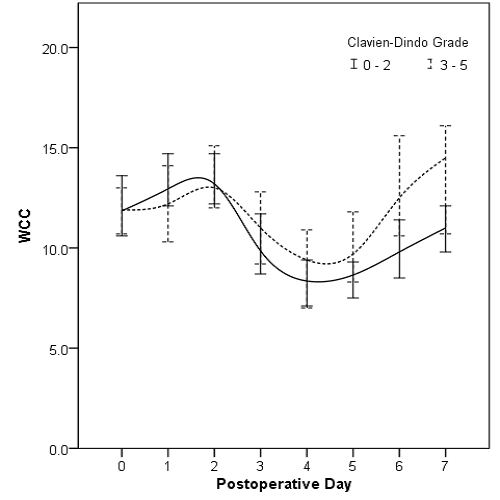
\includegraphics[width=\textwidth]{Figures/crp_comp_WCC_infective_leak0}
		\caption{Patients with \textbf{\underline{no}} POPF}
		\label{fig:crp_comp_WCC_infective_leak0}
	\end{subfigure}
	\hfill
	\begin{subfigure}{0.48\textwidth}
		\centering
		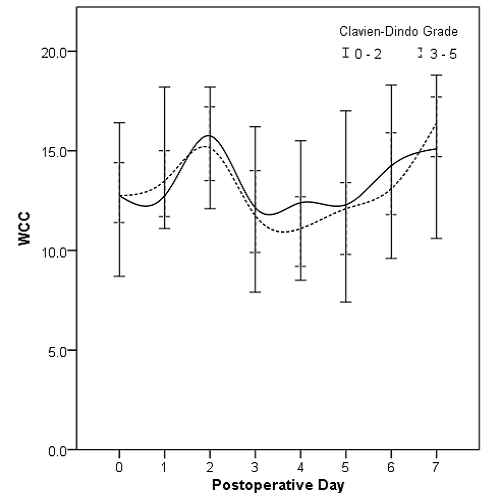
\includegraphics[width=\textwidth]{Figures/crp_comp_WCC_infective_leak1}
		\caption{Patients with POPF}
		\label{fig:crp_comp_WCC_infective_leak1}
	\end{subfigure}
\end{figure}
\vfill
%13/07/15 - Started this table
\begin{table}[h]
	\centering
	\caption{The relationship between postoperative white cell count and infective complications grouped by POPF. (Mann-Whitney U test)}
	\label{table:crp_comp_WCC_vs_infections_popf_y1n0}
	%\renewcommand{\arraystretch}{1.1} %Increases space between rows
	%\setlength{\tabcolsep}{9pt} %sets the space between columns
	\begin{tabular}{| c | c c c | c c c |}
		\hline
		           &       \multicolumn{3}{c|}{POPF Absent}       &      \multicolumn{3}{c|}{POPF Present}       \\
		           & \multicolumn{3}{c|}{Infective Complication} & \multicolumn{3}{c|}{Infective Complication} \\
		Postop Day & No            & Yes           & p            & No            & Yes           & p            \\
		           & (n=85)        & (n=41)        &              & (n=19)        & (n=43)        &  \\ \hline
		0          & 12.1          & 11.9          & 0.843        & 12.6          & 12.6          & 0.658        \\
		           & (9.7 - 14.6)  & (9.8 - 15.6)  &              & (8 - 16.4)    & (10.1 - 15.4) &  \\
		1          & 13.0          & 12.7          & 0.297        & 13.6          & 13.6          & 0.708        \\
		           & (11.6 - 15.8) & (9.5 - 16.4)  &              & (11.1 - 18.2) & (10.6 - 16.4) &  \\
		2          & 13.6          & 13.7          & 0.998        & 14.5          & 14.8          & 0.754        \\
		           & (11.3 - 16.9) & (10.5 - 17.2) &              & (10.8 - 18.2) & (12.4 - 19.3) &  \\
		3          & 9.9           & 11.0          & 0.223        & 12.0          & 11.7          & 0.843        \\
		           & (8.1 - 13.3)  & (8.6 - 14.9)  &              & (7.9 - 16.2)  & (8.2 - 15.3)  &  \\
		4          & 8.4           & 9.4           & 0.095        & 12.1          & 11.1          & 0.523        \\
		           & (6.5 - 10.8)  & (6.8 - 13.4)  &              & (8.5 - 15.5)  & (8.7 - 12.9)  &  \\
		5          & 8.9           & 9.8           & 0.028        & 12.3          & 12.3          & 0.849        \\
		           & (6.6 - 11)    & (7.9 - 13)    &              & (7.4 - 17)    & (9.5 - 14.7)  &  \\
		6          & 9.8           & 12.5          & 0.007        & 14.3          & 13.6          & 0.782        \\
		           & (7.8 - 13.2)  & (9.9 - 16)    &              & (9.6 - 18.3)  & (10.8 - 16.7) &  \\
		7          & 11.2          & 14.6          & 0.003        & 14.9          & 16.4          & 0.302        \\
		           & (9 - 14.1)    & (10.5 - 18.7) &              & (10.6 - 18.8) & (14.5 - 19.4) &  \\ \hline
		\multicolumn{7}{l}{Values are median (inter-quartile range)}                                            \\
		\multicolumn{7}{l}{p - Mann-Whitney U test}
	\end{tabular}
\end{table}
%==============================================================================

%==========Neutrophil-Neutrophil-Neutrophil-Neutrophil-Neutrophil-Neutrophil=====
%Neutrophil trends vs infections in patients with or without popf in a 2-panel figure and table showing median, iqr and p-values below it
\clearpage
\begin{figure}[t]
	\caption{Relationship between postoperative neutrophil count and clinically significant infective complications in patients without (A) and with (B) POPF.}
	\label{fig:crp_comp_Neutrophil_infective_leak}
	\centering
	\begin{subfigure}{0.48\textwidth}
		\centering
		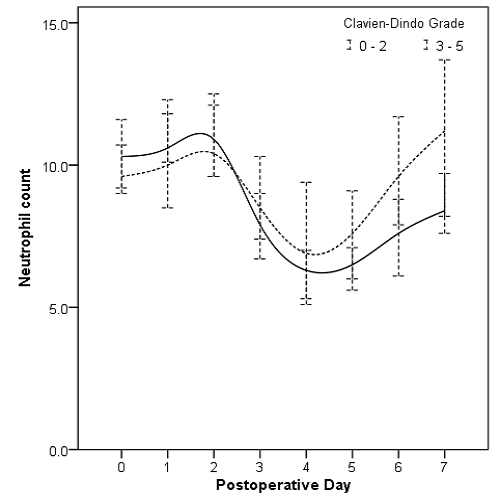
\includegraphics[width=\textwidth]{Figures/crp_comp_Neutrophil_infective_leak0}
		\caption{Patients with \textbf{\underline{no}} POPF}
		\label{fig:crp_comp_Neutrophil_infective_leak0}
	\end{subfigure}
	\hfill
	\begin{subfigure}{0.48\textwidth}
		\centering
		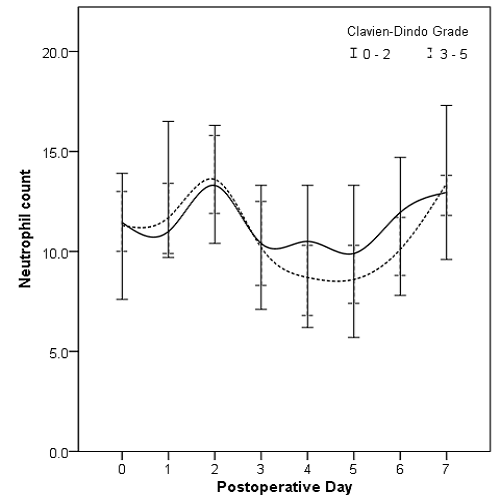
\includegraphics[width=\textwidth]{Figures/crp_comp_Neutrophil_infective_leak1}
		\caption{Patients with POPF}
		\label{fig:crp_comp_Neutrophil_infective_leak1}
	\end{subfigure}
\end{figure}
\vfill
%13/07/15 - Started this table
\begin{table}[h]
	\centering
	\caption{The relationship between postoperative neutrophil count and infectious complications grouped by POPF.}
	\label{table:crp_comp_Neutrophil_vs_infections_popf_y1n0}
	%\renewcommand{\arraystretch}{1.1} %Increases space between rows
	%\setlength{\tabcolsep}{9pt} %sets the space between columns
	\begin{tabular}{| c | c c c | c c c |}
		\hline
		           &       \multicolumn{3}{c|}{POPF Absent}       &      \multicolumn{3}{c|}{POPF Present}       \\
		           & \multicolumn{3}{c|}{Infectious Complication} & \multicolumn{3}{c|}{Infectious Complication} \\
		Postop Day & No           & Yes          & p             & No           & Yes           & p            \\
		           & (n=85)       & (n=41)       &               & (n=19)       & (n=43)        &  \\ \hline
		0          & 10.5         & 9.9          & 0.694         & 11.4         & 11.0          & 0.840 \\
		           & (8.4 - 12.7) & (8.5 - 13.9) &               & (7.3 - 13.9) & (8.6 - 13.5)  &  \\
		1          & 10.6         & 10.4         & 0.517         & 11.3         & 11.6          & 0.375 \\
		           & (9.1 - 13.2) & (7.7 - 14.2) &               & (9.7 - 16.5) & (8.5 - 13.8)  &  \\
		2          & 10.9         & 11.3         & 0.704         & 12.8         & 12.1          & 0.843 \\
		           & (8.7 - 13.9) & (9.4 - 14.2) &               & (8.6 - 16.3) & (10.5 - 16.5) &  \\
		3          & 7.9          & 8.5          & 0.086         & 10.1         & 10.1          & 0.855 \\
		           & (6 - 10.9)   & (7.1 - 12.2) &               & (7.1 - 13.3) & (7 - 13.3)    &  \\
		4          & 6.3          & 7.0          & 0.072         & 10.2         & 9.0           & 0.445 \\
		           & (4.8 - 8.4)  & (5.2 - 10.8) &               & (6.2 - 13.3) & (6.5 - 10.8)  &  \\
		5          & 6.6          & 7.6          & 0.021         & 9.9          & 9.1           & 0.693 \\
		           & (4.7 - 8.3)  & (5.6 - 10.7) &               & (5.7 - 13.3) & (7.1 - 11.3)  &  \\
		6          & 7.6          & 9.6          & 0.004         & 12.0         & 10.5          & 0.675 \\
		           & (5.8 - 9.7)  & (7.5 - 13.1) &               & (7.8 - 14.7) & (8 - 13.1)    &  \\
		7          & 8.7          & 11.6         & 0.001         & 12.4         & 13.4          & 0.412 \\
		           & (6.7 - 10.8) & (7.9 - 16.1) &               & (8.6 - 17.3) & (11.5 - 15.9) &  \\ \hline
		\multicolumn{7}{l}{Values are median (inter-quartile range)}                                          \\
		\multicolumn{7}{l}{p - Mann-Whitney U test}
	\end{tabular}
\end{table}

%==============================================================================

%==========Albumin-Albumin-Albumin-Albumin-Albumin-Albumin-Albumin-Albumin-=====
%Albumin trends vs infections in patients with or without popf in a 2-panel figure and table showing median, iqr and p-values below it
\clearpage
\begin{figure}[t]
	\caption{Relationship between postoperative serum albumin and clinically significant infective complications in patients without (A) and with (B) POPF.}
	\label{fig:crp_comp_Albumin_infective_leak}
	\centering
	\begin{subfigure}{0.48\textwidth}
		\centering
		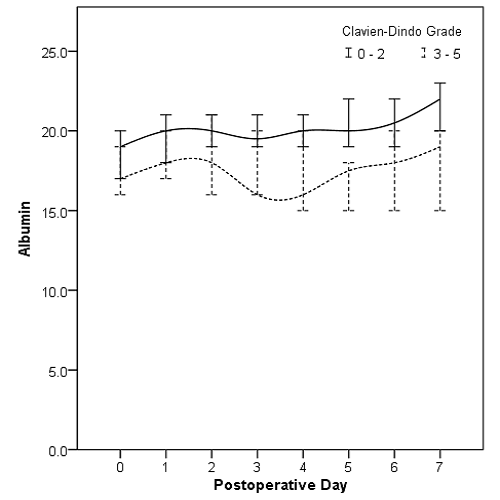
\includegraphics[width=\textwidth]{Figures/crp_comp_Albumin_infective_leak0}
		\caption{Patients with \textbf{\underline{no}} POPF}
		\label{fig:crp_comp_Albumin_infective_leak0}
	\end{subfigure}
	\hfill
	\begin{subfigure}{0.48\textwidth}
		\centering
		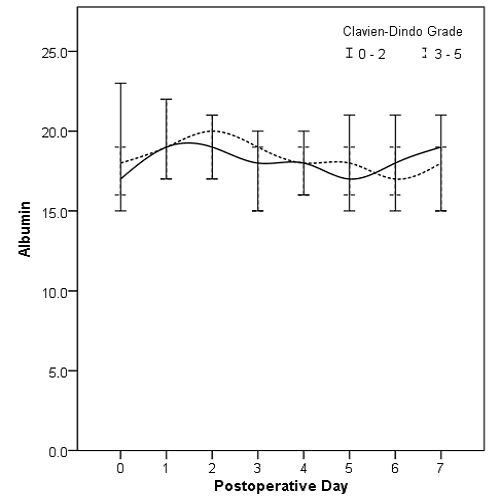
\includegraphics[width=\textwidth]{Figures/crp_comp_Albumin_infective_leak1}
		\caption{Patients with POPF}
		\label{fig:crp_comp_Albumin_infective_leak1}
	\end{subfigure}
\end{figure}
\vfill
%13/07/15 - Started this table
\begin{table}[b]
	\centering
	\caption{The relationship between postoperative serum albumin and infective complications grouped by POPF. (Mann-Whitney U test)}
	\label{table:crp_comp_Albumin_vs_infections_popf_y1n0}
	%\renewcommand{\arraystretch}{1.1} %Increases space between rows
	%\setlength{\tabcolsep}{9pt} %sets the space between columns
	\begin{tabular}{| c | c c c | c c c |}
		\hline
		           &       \multicolumn{3}{c|}{POPF Absent}       &      \multicolumn{3}{c|}{POPF Present}       \\
		           & \multicolumn{3}{c|}{Infective Complication} & \multicolumn{3}{c|}{Infective Complication} \\
		Postop Day & No        & Yes         & p                  & No        & Yes       & p                    \\
		           & (n=85)    & (n=41)      &                    & (n=19)    & (n=43)    &  \\ \hline
		0          & 20        & 17          & 0.101              & 18        & 18        & 0.981                \\
		           & (15 - 22) & (14 - 21)   &                    & (15 - 22) & (15 - 20) &  \\
		1          & 20        & 18          & 0.115              & 20        & 19        & 0.612                \\
		           & (16 - 23) & (15 - 21)   &                    & (17 - 22) & (16 - 23) &  \\
		2          & 20        & 18          & 0.090              & 18        & 19        & 0.545                \\
		           & (17 - 23) & (15 - 21.5) &                    & (15 - 21) & (16 - 22) &  \\
		3          & 20        & 16          & 0.001              & 18        & 19        & 0.689                \\
		           & (17 - 22) & (13 - 20)   &                    & (15 - 20) & (15 - 20) &  \\
		4          & 20        & 16          & $<$0.001           & 17        & 18        & 0.945                \\
		           & (17 - 23) & (14 - 20)   &                    & (16 - 19) & (15 - 20) &  \\
		5          & 20        & 18          & $<$0.001           & 16        & 18        & 0.667                \\
		           & (17 - 23) & (13.5 - 20) &                    & (15 - 20) & (15 - 20) &  \\
		6          & 20        & 18          & 0.001              & 17        & 17        & 0.981                \\
		           & (18 - 24) & (14 - 20)   &                    & (15 - 20) & (15 - 20) &  \\
		7          & 22        & 19          & $<$0.001           & 18        & 18        & 0.655                \\
		           & (18 - 25) & (14 - 20)   &                    & (15 - 20) & (15 - 21) &  \\ \hline
		\multicolumn{7}{l}{Values are median (inter-quartile range)}                                             \\
		\multicolumn{7}{l}{p - Mann-Whitney U test}
	\end{tabular}
\end{table}

%=============================================================================
\clearpage

\subsection{Receiver operating characteristic (ROC) analysis}
Receiver operating characteristic (ROC) analysis was undertaken in order to find the optimum threshold for the relationship between CRP and infective complications in patients without POPF. ROC curves were plotted with CR as a continuous variable and infective complications as a dichotomous outcome variable for postoperative days 3 through 7. 

The area under curve (AUC) was significantly higher than 0.5 for CRP on days 3 though 7. The optimum thresholds along with the corresponding sensitivity, specificity, negative predictive value, positive predictive value, 95\% confidence intervals (CI) and p-values are shown in Table \ref{table:crp_comp_ROC_infections_noPOPF} and the corresponding ROC curves are shown in Fig. \ref{fig:crp_comp_ROC_infection} on p\pageref{fig:crp_comp_ROC_infection}. The thresholds were identified with a bias towards a higher negative predictive value to allow identification of patients who did not develop an infective complication. A CRP level of 125 mg/L on the fourth postoperative day had a sensitivity of 74\% and specificity of 64\% with a negative predictive value of 83\% for predicting infective complications (AUC 0.71, 95\%CI 0.61 - 0.80, p$<$0.001). The AUC improved to 0.80 on day 7 but only with a modest increase in the negative predictive value to 87\%, with corresponding sensitivity, specificity of 65\% and 81\% respectively (95\%CI 0.72 - 0.88, p$<$0.001).

The relationship between CRP on the fourth day and other postoperative events is shown in Table \ref{table:crp_comp_CRP4_vs_LOS}. There were no deaths in this group of patients who did not have a POPF. 

%SPSS results and graphs are stored in crp_complications_graphs_etc.spv file

%========================ROC Curves==========================================
\clearpage
\begin{figure}[t]
	\caption{Receiver operating characteristics curve analysis of C-reactive protein as a marker of postoperative infective complications.}
	\label{fig:crp_comp_ROC_infection}

	\centering
	\begin{subfigure}{0.3\textwidth}
		\centering
		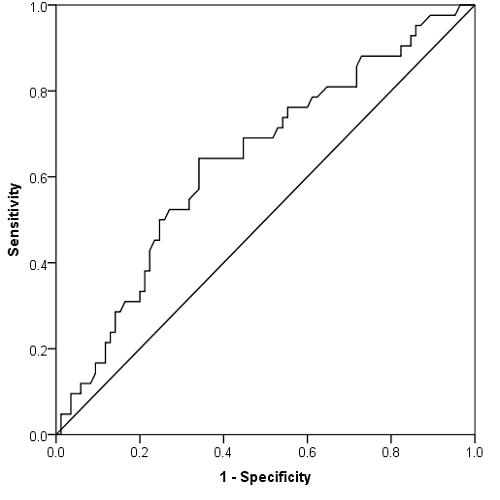
\includegraphics[width=\textwidth]{Figures/crp_comp_ROC_infection_D3}
		\caption{Day 3}
		\label{fig:crp_comp_ROC_infection_D3}
	\end{subfigure}
	\hfill
	\begin{subfigure}{0.3\textwidth}
		\centering
		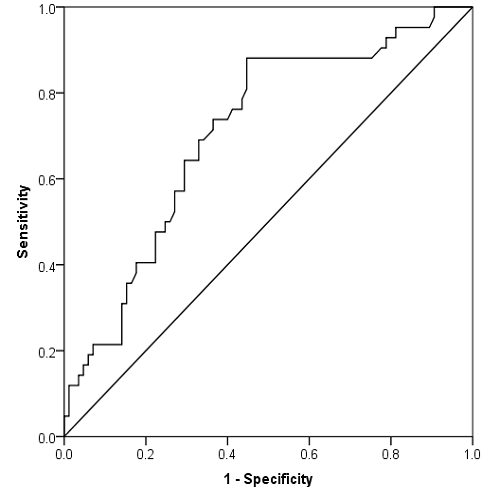
\includegraphics[width=\textwidth]{Figures/crp_comp_ROC_infection_D4}
		\caption{Day 4}
		\label{fig:crp_comp_ROC_infection_D4}
	\end{subfigure}
	\hfill
	\begin{subfigure}{0.3\textwidth}
		\centering
		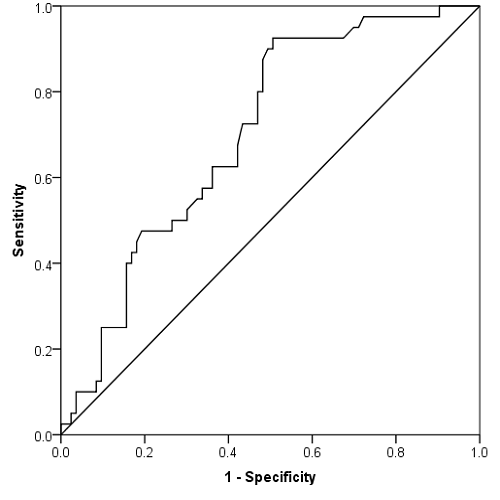
\includegraphics[width=\textwidth]{Figures/crp_comp_ROC_infection_D5}
		\caption{Day 5}
		\label{fig:crp_comp_ROC_infection_D5}
	\end{subfigure}
	\begin{subfigure}{0.3\textwidth}
		\centering
		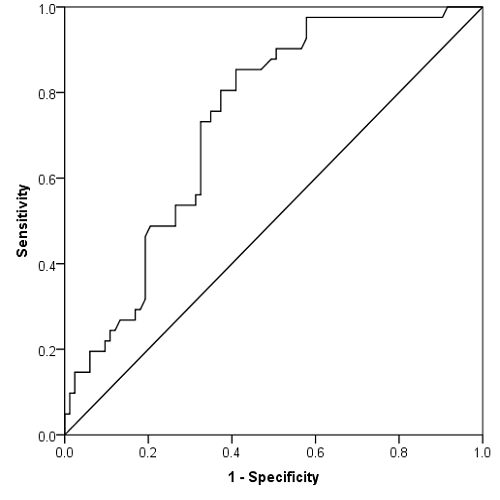
\includegraphics[width=\textwidth]{Figures/crp_comp_ROC_infection_D6}
		\caption{Day 6}		
		\label{fig:crp_comp_ROC_infection_D6}
	\end{subfigure}
	\begin{subfigure}{0.3\textwidth}
		\centering
		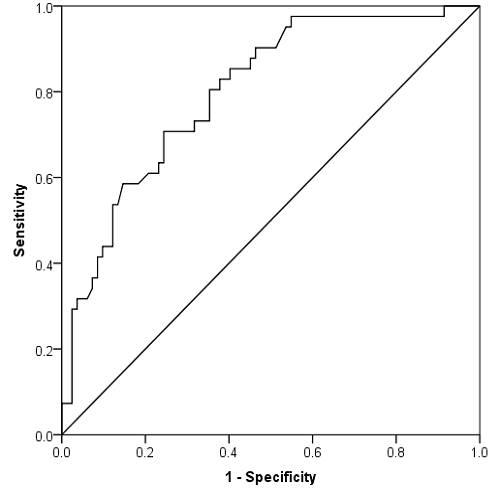
\includegraphics[width=\textwidth]{Figures/crp_comp_ROC_infection_D7}
		\caption{Day 7}
		\label{fig:crp_comp_ROC_infection_D7}
	\end{subfigure}
\end{figure}
\vfill
%07/07/15 - Started this table
\begin{table}[h]
	\centering
	\caption{Receiver operating characteristics curve analysis of C-reactive protein as a marker of postoperative infective complications in patients who did not develop a POPF}
	\label{table:crp_comp_ROC_infections_noPOPF}
	\renewcommand{\arraystretch}{1.4} %Increases space between rows
	%\setlength{\tabcolsep}{9pt} %sets the space between columns
	\begin{tabular}{| c | c c c | c c c c c |}
		\hline
		Day & AUC  & p        & 95\% CI     & CRP & Spec. & Sens. & NPV  & PPV               \\ \hline
		3   & 0.64 & 0.011    & 0.54 - 0.74 & 178 & 0.66  & 0.64  & 0.79 & 0.48              \\
		4   & 0.71 & $<$0.001 & 0.61 - 0.80 & 125 & 0.64  & 0.74  & 0.83 & 0.50              \\
		5   & 0.70 & $<$0.001 & 0.61 - 0.80 & 107 & 0.64  & 0.63  & 0.78 & 0.45              \\
		6   & 0.73 & $<$0.001 & 0.65 - 0.82 & 92  & 0.68  & 0.73  & 0.84 & 0.53              \\
		7   & 0.80 & $<$0.001 & 0.72 - 0.88 & 87  & 0.65  & 0.81  & 0.87 & 0.52              \\ \hline
		\multicolumn{9}{l}{AUC - Area under curve, Spec. - Specificity, Sens. - Sensitivity} \\
		\multicolumn{9}{l}{NPV - Negative Predictive Value, PPV - Positive Predictive Value}
	\end{tabular}
\end{table}
%=============================================================================

%===================CRP Day 4 vs LOS=========================================

%12/07/15 - Started this table
\begin{table}[p]
	\centering
	\caption{The relationship between CRP on Day 4 and other postoperative events in patients with no POPF.}
	\label{table:crp_comp_CRP4_vs_LOS}
	\renewcommand{\arraystretch}{1.4} %Increases space between rows
	\setlength{\tabcolsep}{9pt} %sets the space between columns
	\begin{tabular}{|l l  c c r |}
		\hline
		                      &          & \multicolumn{2}{c}{Day 4 CRP (mg/l)} &  \\
		                      &          & $\leq$125   & $>$125                   & \textit{p}   \\ \hline
		Postoperative stay    & Days     & 12 (9 - 16) & 15 (13 - 26)             & $<$0.001$^a$ \\
		(days)                & $\leq$14 & 43 (66.2\%) & 30 (49.2\%)              & $<$0.054$^b$ \\
		                      & $>$14    & 22 (33.8\%) & 31 (50.8\%)              &  \\
		Critical care stay    & Days     & 6 (4 - 7)   & 7 (5 - 10)               & 0.001$^a$    \\
		(days)                & $\leq$7  & 57 (87.7\%) & 38 (62.3\%)              & 0.001$^b$    \\
		                      & $>$7     & 8 (12.3\%)  & 23 (37.7\%)              &  \\
		Crit. care admissions & 1        & 60 (92.3\%) & 48 (78.7\%)              & 0.029$^b$    \\
		                      & $>$1     & 5 (7.7\%)   & 13 (21.3\%)              &  \\
		Reoperation           & No       & 63 (96.9\%) & 57 (93.4\%)              & $<$0.359$^b$ \\
		                      & Yes      & 2 (3.1\%)   & 4 (6.6\%)                &  \\ \hline
		\multicolumn{5}{l}{a - Mann-Whitney U test; b - Chi-square test}
	\end{tabular}
	\medskip
	\begin{flushleft}
		In patients who did not develop a postoperative pancreatic fistula (n=126), CRP $\leq$ 125 mg/l on the fourth postoperative day was associated with shorter stay in hospital, fewer days in critical care and lower rate of readmission to critical care.
	\end{flushleft}
\end{table}





%Quick analysis of CPET vs postop CRP - maybe one table
%ROC analysis of CRP vs LOS
%Multivariate analysis of CRP as continuous or categorical vs complications, 
\clearpage
\section{Discussion}

The results of the present study show that the severity of the postoperative systemic inflammatory response as measured by serial serum CRP levels in the first week is associated with postoperative complications after pancreaticoduodenectomy. While numerous studies have reported on a variety of methods to predict as well as diagnose POPF, few have reported on the role of CRP in predicting complications other than POPF.

The introduction of the ISGPF definition for POPF has made the diagnosis of this complication simple and uniform. The rate of POPF before the standardised definition was introduced varied anywhere between 2\% and 40\%. However, in the post-ISGPF era, the rate of POPF in published literature has remained approximately 25\%. The sole criterion for the diagnosis of POPF is a drain amylase content on or after the third postoperative day three times the upper limit of normal for serum amylase in the testing laboratory. 

In the present study, while CRP was significantly greater in patients with POPF, this difference did not occur until the second postoperative day and therefore had no further clinical use in the prediction of this complication. The early rise in CRP in patients who developed a POPF is expected as the most common risk factors for POPF are encountered intra-operatively including soft pancreatic texture, small pancreatic duct size and operative blood loss. Soft pancreatic texture has in fact been reported to be associated with elevated CRP levels after pancreaticoduodenectomy.\parencite{murakami_soft_2008}

However, the magnitude of increase in CRP during the first postoperative week was not associated with the severity of POPF. This lack of association appears to suggest that the determinants of the severity of POPF may occur later in the postoperative course and are not related to the magnitude of the initial systemic inflammatory response.

The presumed cascade of events following a POPF involves accumulation of amylase rich fluid in the peritoneal cavity around recently dissected tissues and ligated blood vessels. This can lead to localised collections that can become secondarily infected, result in erosion of blood vessels resulting in post-pancreatectomy haemorrhage, result in delayed gastric emptying or postoperative ileus as well as respiratory complications including sympathetic pleural effusions or pneumonic consolidation. In fact, most large series report a close association between POPF and PPH with the latter often following the former. The eventual outcome in patients with POPF is often determined by the cascade of complications associated with the POPF itself. In fact, all deaths in this study were in patients who developed POPF.

However, in patients without a POPF, CRP in the first week after surgery was associated with infective complications and preceded the clinical manifestation of complications. The postoperative course of patients who do not develop a POPF is not dissimilar to that in patients undergoing other major gastrointestinal resectional surgery such as colorectal or oesophago-gastric surgery. The impact of the systemic inflammatory response and the compensatory anti-inflammatory response in these patients is not confounded by the presence of POPF. Our results show that once the absence of POPF is confirmed by normal drain amylase content on the third postoperative day, serum CRP on the next (fourth) postoperative day less than 125 mg/L had a negative predictive value of 83\% in excluding an infective complication. 

The results of this study are similar to the findings of Welsch and co-workers who analysed 688 patients undergoing a variety of pancreatic resections with pancreaticojejunal anastomosis.\parencite{welsch_persisting_2008} They compared 91 patients who developed an 'inflammatory postoperative complication' with a random subset of 60 consecutive pancreatic resections. They reported that a threshold of 140 mg/L serum CRP level on the fourth postoperative day had the best diagnostic accuracy for the prediction of inflammatory postoperative complications (sensitivity 69.5\%, specificity 87.1\%, positive predictive value 48.7\% for an estimated prevalence of 15\%). However, the definitions used for POPF in this study were different from the ISGPF definition and the authors did not report on the predictive ability of CRP in the presence or absence of a POPF. Moreover, Grade A and B POPF were not included in the analysis. Our results clearly demonstrate that early CRP elevation occurs in all grades of POPF with no difference between the different grades.

In the present study, preoperative systemic inflammation as measured by the modified Glasgow Prognostic Score was not associated with infective complications. A preoperative acute phase response has been reported to be associated with an exaggerated postoperative systemic inflammatory response and septic complications. \parencite{haupt_association_1997} The modified Glasgow Prognostic Score, a validated measure of preoperative systemic inflammation, has also been reported to be associated with postoperative infective complications in patients undergoing curative colorectal resections.\parencite{moyes_preoperative_2009} The lack of association between the modified Glasgow Prognostic Score and complications in the present study may have been due to the multiple factors that are responsible for preoperative systemic inflammation in these patients including obstructive jaundice, cholangitis, biliary drainage procedures and pancreatitis consequent to intervention or pancreatic duct obstruction by tumours. These findings are similar to those reported by Dutta and co-workers who did not find any relationship between preoperative systemic inflammation and postoperative complications in patients undergoing oesophago-gastric surgery.\parencite{dutta_persistent_2011}

The difference in white cell count and neutrophil count was not clinically significant between patients who did or did not have an infective complication. This finding is similar to one of the earliest reports on the role serial CRP measurements in predicting septic complications after surgery.\parencite{mustard_c-reactive_1987} as well as in several subsequent reports. \parencite{matthiessen_increase_2008, welsch_persisting_2008, dutta_persistent_2011} The temporal association between CRP and infective complications may reflect the sensitivity of CRP as a marker of systemic inflammation. This study was not designed to look at inflammatory markers later in the postoperative period. However, Mustard and co-workers monitored CRP, white cell count and temperature for 14 days after surgery and found that CRP was the only reliable marker of septic complications.

Several mechanisms have been postulated to explain the association between postoperative CRP and complications. The most common explanation is that the CRP rise is consequent to tissue ischaemia, necrosis at the anastomotic site, bacterial translocation from the gut or bacterial infection of wounds. However, our findings and that of other authors show that the difference in CRP occurs very early in the postoperative period before infective complications become clinically manifest. 

More recently, the compensatory anti-inflammatory response with the associated immunosuppressive effects has been recognised as a possible factor in predisposing the patient to infective complications and delayed wound healing. Such an anti-inflammatory response is proportional to the initial systemic inflammatory response and therefore patients with an exaggerated inflammatory response in the immediate aftermath of surgery may be at increased risk of developing complications. Mokart and co-workers studied trends in inflammatory cytokine levels in the serum of 30 patients undergoing major abdominal surgery for cancer. They reported that the levels of anti-inflammatory cytokines IL-10 and IL-1ra were significantly greater in patients who developed infective complications and were correlated with IL-6 levels on the first postoperative day. T-cell function is also depressed after surgical trauma and the degree of suppression is related to the initial pro-inflammatory response and IL-6.\parencite{faist_immunosuppression_1997} The complex interactions between the pro and anti-inflammatory processes, neurohormonal factors of the stress response, the role of the blood-gut barrier in bacterial translocation, local factors including tissue ischaemia and damage, the immunological effects of anaesthesia, blood transfusion and hypothermia remain the subject of ongoing research.\parencite{buttenschoen_effect_2010}

%=========Strengths and limitations==========================
One of the most important strengths of this study is the separate analysis of infective complications in patients who did not develop a POPF. Other strengths of this study include the homogeneous cohort of patients all of who underwent a pancreaticoduodenectomy, the serial measurements of CRP on every day of the first postoperative week, prospective record of complications and use of the ISGPF definition for POPF. We did not measure levels of other inflammatory cytokines routinely in these patients. Future work should be aimed at characterising the inflammatory cytokine profile after pancreaticoduodenectomy to identify potential targets for immunomodulation in the perioperative period. 

In summary, the advent of enhanced recovery protocols in surgery including pancreatic surgery requires the early identification of patients not only at increased risk of complications but also those who are likely to have an uncomplicated course. This allows early identification of patients who are expected to continue on the enhanced recovery pathway and allocation of resources to improve the management of patients who are likely to develop complications. This study shows that CRP on the third postoperative day is associated with infective complications in patients undergoing pancreaticoduodenectomy who do not develop a POPF but not in patients with a POPF.

%% Discussion

\chapter{Discussion}
\label{ch_discussion}

\lhead{Chapter \ref{ch_discussion}. \emph{Discussion}} % This is for the header on each page - perhaps a shortened title

\clearpage
%----------------------------------------------------------------------------------------
\section{Aims of thesis}

The overall aim of the thesis was to examine the inter-relationships between preoperative clinico-pathological characteristics including cardiopulmonary exercise physiology, obstructive jaundice, body composition and preoperative systemic inflammation and post-operative complications and the post-surgical systemic inflammatory response in patients undergoing pancreaticoduodenectomy.

The present work also examined the factors that affect cardiopulmonary exercise physiology in order to enable a better understanding of the complex pathophysiology in these patients that is a consequence of the interaction of the patient's chronic conditions with the acute derangements brought on by pancreatic disease, including obstructive jaundice.

%################################################################################
\section{Clinical utility of CPET in predicting postoperative complications}
%################################################################################

\subsection{Risk assessment and predicting complications}

The results presented in chapter \ref{ch_cpet_outcomes} demonstrated that cardiopulmonary exercise testing has a role in identifying high risk patients who are more likely to develop complications, stay longer in hospital and are less likely to receive adjuvant therapy after pancreaticoduodenectomy. 
These findings have since been replicated by other authors examining the role of cardiopulmonary exercise testing in pancreatic surgery. 

Ausania and co-workers evaluated the role of cardiopulmonary exercise testing in 122 patients who underwent a pancreaticoduodenectomy \parencite{ausania_effects_2012}
Low $\dot{V}_{O_2}$AT ($<$10.1 ml/kg/min) was the only independent predictor of a postoperative pancreatic fistula.
The incidence of a postoperative pancreatic fistula was 45\% in patients with a low $\dot{V}_{O_2}$AT while it was only 19\% in patients with a normal $\dot{V}_{O_2}$AT (p=0.02).
The association between $\dot{V}_{O_2}$AT and postoperative pancreatic fistula was independent of pancreatic duct size, body mass index, obstructive jaundice or preoperative biliary drainage.
They also reported in a separate study of 50 patients that complication  rates were higher in patients with a low $\dot{V}_{O_2}$AT undergoing palliative surgical bypass for advanced pancreatic cancer \parencite{ausania_double_2012}.

Junejo and co-workers identified elevated $\dot{V}_E/\dot{V}_{CO_2}$ to be an independent predictor of 30-day mortality after pancreaticoduodenectomy in their study that included 64 patients who had undergone cardiopulmonary exercise testing \parencite{junejo_cardiopulmonary_2014}.
$\dot{V}_{O_2}$AT and $\dot{V}_{O_2}$Peak  were not related to mortality or complications in this study.
However, they also noted that a high $\dot{V}_E/\dot{V}_{CO_2}$ was also associated with poor long-term survival.

\subsection{Assessing impact of prehabilitation or neoadjuvant treatment}
The results of our work as well as that of several others over the past 2 decades support the use of cardiopulmonary exercise testing as a clinical risk assessment tool in patients undergoing major surgery.
However, as presented in the subsequent chapters of this thesis, a better understanding of the determinants of aerobic capacity as well as the perioperative systemic inflammatory response will enable clinicians to identify high risk patients and optimise their perioperative care.

In a recent study of 8266 patients undergoing pancreaticoduodenectomy in the United States, Tzeng and co-workers reported that a third (3033) were of borderline fitness as a consequence of advanced age ($>$ 80), poor performance status, weight loss $>$ 10\%, pulmonary disease, recent myocardial infarction/angina, stroke history, and/or preoperative sepsis. 
Major complications (31.3 vs. 26.2\%) and mortality (4.1 vs. 2.3\%) were greater in patients with borderline fitness \parencite{tzeng_morbidity_2014}.
The authors recommended that surgeons identify these patients early, institute interventions to optimise their comorbidities and enrol these patients for prehabilitation. 

Neoadjuvant treatments were associated with significant reduction in $\dot{V}_{O_2}$AT and $\dot{V}_{O_2}$Peak in patients with rectal cancer \parencite{west_effects_2014} and oesphago-gastric cancer \parencite{jack_effect_2014}.
West and co-workers used prehabilitation to return aerobic capacity to baseline levels in patients with locally advanced rectal cancer undergoing neo-adjuvant chemoradiotherapy.
They used cardiopulmonary exercise testing to monitor the impact of neo-adjuvant treatment and prehabilitation \parencite{west_effect_2015}.
Neoadjuvant therapy in borderline resectable pancreatic cancer is the subject of several trials with generally promising results \parencite{evans_preoperative_2008, gillen_preoperative/neoadjuvant_2010, golcher_neoadjuvant_2015, kim_multi-institutional_2013, sahora_phase_2014}.

It is likely that the impact of such treatment on fitness in these patients will be similar to that observed in patients with colorectal and oesophago-gastric cancer.
Prehabilitation would play an important role in improving outcomes in these patients while cardiopulmonary exercise testing will serve as an important clinical tool to objectively measure the impact of prehabilitation.

\subsection{Assessing impact on long-term survival}

Poor aerobic capacity is associated with reduced long-term survival after abdominal aortic aneurysm surgery \parencite{tang_cardiopulmonary_2012, grant_cardiopulmonary_2015}.
There is some evidence that cardiopulmonary exercise testing may predict long-term survival after pancreaticoduodenectomy for pancreatic cancer \parencite{junejo_cardiopulmonary_2014}.
Reduced aerobic capacity was also associated with poor survival in patients with lung cancer \parencite{jones_peak_2010}.

While the an elevated preoperative systemic inflammatory response has been shown to have an adverse impact on long-term survival in patients with pancreatic cancer both in those who underwent potentially curative surgery or palliation, the impact of aerobic capacity and comorbidity on long-term survival in patients with pancreatic cancer is less clear.
Some have suggested that comorbidity was associated with shorter survival in patients with pancreatic cancer \parencite{dias-santos_charlson_2015}.
However, other authors have reported that the relatively short median survival after pancreatic cancer is not affected by comorbidity in patients who underwent potentially curative surgery \parencite{kos_evaluation_2014}

The relationship between aerobic capacity and cancer-survival is important as it provides for a relatively easy therapeutic target.

% Different surgeries and patient groups may need different thresholds for risk prediction
% Done - CPET and long-term survival in PDAC
% Why is low $\dot{V}_{O_2}$ likely to leak - pancreatic perfusion 
%high lactate - popf de_schryver_early_2015

%karoliska - ansorge_early_2012
- better understanding of physiology
- role of sytemic inflammation \parencite{van_heek_hospital_2005, ho_effect_2003, birkmeyer_surgeon_2003, halm_is_2002}
- impact of sarcopenic-obesity \parencite{joglekar_sarcopenia_2015, reisinger_sarcopenia_2015, gonzalez_obesity_2014}
- role of tumour related factors \parencite{williams_surgical_2014}


%################################################################################
\section{Prehabilitation, improving aerobic capacity and mitigating risk}
%################################################################################
In Chapters \ref{ch_cpet_jaundice} and \ref{ch_bodycomp} we examined the preoperative patient factors that had an adverse effect on aerobic capacity.
A better understanding of the factors that affect $\dot{V}_{O_2}$ may identify potential therapeutic targets or modifiable risk factors that may be used to improve patient fitness and mitigate the risks of surgery.
We found that female sex, high body mass index, anaemia, presence of cancer and elevated CRP were all associated with either a low $\dot{V}_{O_2}$AT or a low $\dot{V}_{O_2}$Peak.

%################################################################################
\subsection{Obstructive jaundice}
%################################################################################
In our opinion, the most important observation made in chapter \ref{ch_cpet_jaundice} is the lack of association between obstructive jaundice and poor aerobic fitness. 
In chapter \ref{ch_outcomes} we reported that obstructive jaundice was not associated with increased incidence of postoperative complications or prolonged hospital stay. 

We are aware of only one other published study looking at cardiopulmonary exercise testing and peripheral oxygen extraction in jaundiced versus non-jaundiced patients undergoing pancreaticoduodenectomy. 
Junejo and co-workers reported that peripheral oxygen extraction was normal during exercise in patients with malignant obstructive jaundice.\parencite{junejo_peripheral_2014} 
Preoperative biliary drainage is unlikely to improve aerobic fitness or modify their cardiopulmonary response to exercise/surgery \parencite{parker_serum_2014}.

We also demonstrated the immunosuppressive effects of obstructive jaundice on the postoperative systemic inflammatory response in chapter \ref{ch_pre_post_sirs}. 
To our knowledge, this is the first detailed study of the postoperative systemic inflammatory response in jaundiced versus non-jaundiced patients undergoing pancreaticoduodenectomy.

In their, appropriately titled paper \textit{`The Quandary of Preresection Biliary Drainage for Pancreatic Cancer'}, the authors discuss the complex physiological effects of obstructive jaundice, its impact on immune function and the differences between findings in animal studies and humans \parencite{tol_quandary_2012}.
However, they also review recent literature where there appears to be overwhelming evidence that preoperative biliary drainage increases the incidence of postoperative complications, especially infective complications. \parencite{van_der_gaag_preoperative_2010, arkadopoulos_preoperative_2014, fujii_preoperative_2015, furukawa_negative_2015}.


Our results support the emerging view that routine preoperative biliary drainage should no longer be performed in all patients scheduled to undergo a pancreaticoduodenectomy.

%################################################################################
\subsection{Systemic inflammation}
%################################################################################
We reported on the preoperative factors affecting postoperative systemic inflammation in chapter \ref{ch_pre_post_sirs} and the clinical utility of monitoring trends in the early postoperative systemic inflammatory response in predicting complications in chapter \ref{ch_crp_comp}.

Preoperative systemic inflammation is increasingly recognised as playing an important role in determining not only long-term outcomes but also short-term outcomes after cancer surgery \parencite{kubo_elevated_2013, mohri_correlation_2014, moyes_preoperative_2009, neal_preoperative_2011, vashist_glasgow_2010,  haupt_association_1997}.
While we did not find an association between elevated preoperative systemic inflammation in our cohort of patients, we demonstrated in chapter \ref{ch_pre_post_sirs} that preoperative systemic inflammation had a significant impact on  the magnitude of the postoperative inflammatory response.
This supports the theory that abnormal systemic inflammation is a continuum that starts in the preoperative phase and continues into the postoperative phase.

It would appear that preoperative patient factors affect the postoperative systemic inflammatory response independent of intra-operative factors or postoperative complications. 
The mechanisms underlying the association between pre- and post-operative systemic inflammation require further study.

%################################################################################
\subsection{Body composition}
%################################################################################
Overweight and obese patients had significantly lower $\dot{V}_{O_2}$AT and $\dot{V}_{O_2}$Peak in spite of no significant increase in known cardiac or respiratory comorbidities. 
We present a detailed analysis of the relationship between body composition and preoperative cardiopulmonary exercise testing in chapter \ref{ch_bodycomp}.
This has not been reported before in surgical patients to the best of our knowledge. 

The loss of skeletal muscle mass in patients with pancreatic cancer and spurious correlation with obesity due to correction for total body weight may partly explain the low $\dot{V}_{O_2}$ in these patients. 
Low aerobic capacity as measured by cardiopulmonary exercise testing must be interpreted with caution in overweight/obese patients and in patients with pancreatic cancer. 
This is especially true for $\dot{V}_{O_2}$ that has been scaled for total body weight.
Further studies must evaluate other parameters such as $O_2$Pulse or $\dot{V}_E/\dot{V}_{O_2}$ for their ability to predict postoperative outcomes. 
The proportion of obese patients undergoing major surgery is increasing. 
Moreover, sarcopenia and sarcopenic-obesity are recognised as an important adverse prognostic feature in pancreatic cancer \parencite{tan_sarcopenia_2009, peng_impact_2012} and is associated with increased postoperative complications after pancreaticoduodenectomy \parencite{joglekar_sarcopenia_2015, pausch_cachexia_2012}.
Sarcopenia was also an independent risk factor for an elevated postoperative systemic inflammatory response in patients with colorectal cancer \parencite{reisinger_sarcopenia_2015}.

Our results suggest that poor performance at cardiopulmonary exercise testing may not necessarily be related to only cardiac or pulmonary function. 
Body composition appears to not only affect aerobic capacity but also systemic inflammation. 
Improvements in body composition are achievable through nutritional supplementation \parencite{machado_whey_2015} as well as increased physical activity.



%################################################################################
\subsection{Anaemia}
%################################################################################

Measures other than exercise may also improve aerobic capacity. 
Correction of anaemia was associated with an improvement in $\dot{V}_{O_2}$AT by 0.39 ml/kg/min for every 1 gm/dl improvement in haemoglobin \parencite{wright_cardiopulmonary_2014}. 
While anaemia did not change the effect of aerobic exercise in improving physical performance, the overall aerobic fitness was significantly lower in anaemic patients than in patients with normal haemoglobin \parencite{bellotto_anemia_2011}.
However, perioperative blood transfusion in pancreatic cancer patients was associated with poorer long-term outcomes \parencite{kneuertz_effects_2011, sutton_perioperative_2014}.

While iron supplementation is associated with correction of anaemia and reduction in the requirement for blood transfusion, the role of preoperative iron supplementation in improving outcomes is unclear. 
Further randomised controlled trials investigating the short-term and long-term consequences of preoperative iron supplementation in patients undergoing cancer surgery are required before this becomes accepted clinical practice \parencite{beris_perioperative_2008,hallet_impact_2014}.

%################################################################################
\subsection{Aerobic exercise}
%################################################################################

West and co-workers used prehabilitation to return aerobic capacity to baseline levels in patients with locally advanced rectal cancer undergoing neo-adjuvant chemoradiotherapy \parencite{west_effect_2015}.
Moderate aerobic and resistance exercises and protein supplementation started 4 weeks before surgery was noted to improve postoperative functional exercise capacity in patients undergoing colorectal cancer surgery \parencite{gillis_prehabilitation_2014}.
Exercise programs as short as 4 weeks in duration have been reported to improve aerobic capacity by upto 10\%  measured objectively by cardiopulmonary exercise testing.
This could potentially move approximately 30\% of high risk patients into the low risk category \parencite{dunne_pmo-029_2012}.

A recent consensus statement by the `Exercise Prehabilitation in Colorectal Cancer Delphi Study Group' in the United Kingdom showed agreement between colorectal surgeons that prehabilitation must form an important part of the preparation of elective patients for major surgery \parencite{boereboom_forming_2015}. 
The surgeons also agreed that improving aerobic capacity is likely to improve outcomes but recommended that further studies were needed before this became established clinical practice.

%%################################################################################
%Moreover, low aerobic capacity was not associated with documented cardiovascular or respiratory comorbidity or with an elevated POSSUM physiology score.
%It is possible that most patients with significant cardiac or respiratory comorbidity were identified as unsuitable for surgery and therefore were never subject to cardiopulmonary exercise testing. 
%Alternatively, it is possible that these patients did very poorly at cardiopulmonary exercise testing and this, in addition to their cardiorespiratory medical history precluded them from surgery.
%We did not include any patients who did not have an operation and this may have introduced a selection bias.
%%################################################################################

%################################################################################
\section{Improving outcomes after pancreaticoduodenectomy}
%################################################################################

\subsection{Centralisation and Specialisation}

One of the biggest factors in improving both short-term and long-term outcomes after cancer surgery has been the centralisation of cancer cancer and the associated specialisation of surgeons. 

Birkmeyer and co-workers reported in 1999 that hospital volume was not only related to postoperative mortality and morbidity but also to long-term cancer survival in patients undergoing pancreaticoduodenectomy.


\subsection{Early and aggressive management of complications}

Several recent studies have demonstrated the value of monitoring trends in postoperative CRP levels in predicting complications after pancreaticoduodenectomy.
These studies performed at large, specialist centres, have used a combination of postoperative CRP and drain amylase levels to identify patients who are at the least risk of developing a Grade B/C pancreatic fistula \parencite{hiyoshi_usefulness_2013, ansorge_diagnostic_2014, kosaka_multivariate_2014}.

Our approach to interpreting the postoperative systemic inflammatory reponse has been different from the above mentioned studies. 
We demonstrated in chapter \ref{ch_crp_comp} that postoperative CRP did not predict the severity of a pancreatic fistula and did not have any clinical utility in the prediction of a POPF (section \ref{Postoperative CRP vs. POPF}).
However, we demonstrated a clear role for the use of postoperative CRP in predicting infective complications in the absence of a POPF. 

In summary the combination of a low CRP and absence of POPF reduces the likelihood of any other infective complications and identifies patients who are suitable for early discharge.
Such patients will also be more likely to benefit from a full course of adjuvant chemotherapy although this requires further study.

Postoperative complications and the associated systemic inflammatory response are associated with early recurrence and poor-survival after colorectal \parencite{artinyan_infectious_2015, mcardle_impact_2005}, gastric \parencite{hayashi_impact_2015,kubota_prognostic_2014}  and pancreatic cancer surgery \parencite{aoyama_impact_2015, kamphues_postoperative_2012}.

Early recognition and aggressive management of complications is therefore important in mitigating the harmful long-term effects of such adverse events and the associated inflammation. 

\subsection{Enhanced Recovery Programmes}


- centralisation
- specialisation
- early rescue and aggressive management of complications \parencite{gouma_rates_2000}



\subsection{Intra-operative care}

The results of chapter \ref{ch_cpet_outcomes} and the work of Ausania and co-workers appeared to suggest a link between reduced oxygen delivery and increased incidence of pancreatic fistula. 
We hypothesised that tissue hypoperfusion may have played a role in the poor healing of the pancreatico-jejunal anastomosis. 

Reyad and co-workers performed a randomised trial to examine the effect of intra-operative dobutamine infusion during pancreaticoduodenectomy on splanchnic perfusion, hemodynamics, and overall postoperative outcome \parencite{reyad_effect_2013}. 
They reported that intra-operative dobutamine use was associated with improved global oxygen delivery as measured by arterial and venous blood gases, splanchnic perfusion as measured by gastric tonometry and postoperative complications.
It was interesting to note that the incidence of anastomotic leak was 30\% in the control group, 15\% in the group that received 3$\mu$g/kg/min of dobutamine and 5\% in the group that received 5$\mu$g/kg/min of dobutamine (p$<$0.05). The overall complication rate also decreased from 70\% in the control group to 40\% and 20\% in the dobutamine groups (p$<0.05$).

However, the benefit of goal-directed therapy to improve organ perfusion and oxygen delivery in improving postoperative outcomes remains unclear \parencite{grocott_perioperative_2013, pearse_effect_2014}. 
A recent randomised controlled trial evaluated the role of goal-directed therapy in high-risk patients undergoing major elective surgery that targeted individualised oxygen delivery \parencite{ackland_individualised_2015}.
The study did show that patients whose postoperative oxygen delivery was similar to their preoperative values had fewer complications.
However, oxygen delivery was not influenced by goal-directed therapy as any beneficial effect of the intervention was lost with the autonomic nervous system changes that accompanied the increased intravenous fluids and inotropes in the treatment cohort.









\subsection{Post-operative care}


\section{Future directions}


%Early recognition of patients at increased risk of postoperative complications facilitates prompt initiation of appropriate treatment and judicious allocation of critical care resources. 
%Moreover, identification of patients who are unlikely to develop a major postoperative complication allows their progress on enhanced recovery pathways with the benefits of rapid recovery, reduced morbidity and early discharge. 
%These patients are also more likely to receive adjuvant therapy without undue delay. 
%Recognition of these low risk patients helps improve outcomes, reduces hospital costs and releases valuable resources for the care of high risk patients. 
%The results reported in Chapter [ss] demonstrate the value of early post-operative C-reactive protein in identifying patients who are more likely to develop an infective complication. 
%The results show that CRP is only useful in the absence of a postoperative pancreatic fistula. 
%The combination of low drain amylase and low CRP on the third postoperative day identifies patients who do not have a pancreatic fistula and are less likely to develop an infective complication. 



%----------------------------------------------------------------------------------------
%	THESIS CONTENT - APPENDICES
%----------------------------------------------------------------------------------------

\addtocontents{toc}{\vspace{2em}} % Add a gap in the Contents, for aesthetics

\appendix % Cue to tell LaTeX that the following 'chapters' are Appendices

%\chapter{Visual Basic for Applications For CPET Analysis} % Main appendix title
\label{AppendixExcelMacros} % For referencing this appendix elsewhere, use \ref{AppendixA}
\lhead{Appendix \ref{AppendixExcelMacros}. \emph{Excel VBA For CPET Analysis}} % This is for the header on each page - perhaps a shortened title
\clearpage
%------------------------------------------

\setstretch{1.0}
The following VBA code was written by me to facilitate detailed analysis of large volumes of raw CPET data that would not have been otherwise available from the final report generated for clinical use. Where necessary, I have used information from the MSDN knowledgebase and internet fora to supplement my knowledge of coding.

\begin{lstlisting}
Option Explicit
Sub RenameSortSheets() 
   Dim ws As Worksheet
   Dim strName() As String
 
   For Each ws In Worksheets
     If ws.Range("$B$1").Value = "" Then
       Exit Sub
     End If
     If ws.Name <> "aaa_main" Then
       strName = Split(CStr(ws.Range("$B$1").Value), "(")
       ws.Name = LCase(strName(0))
       ws.Activate
       ws.Range("B4").Select
       ActiveWindow.FreezePanes = True
     End If
   Next ws
 
   Dim N As Integer
   Dim M As Integer
   Dim FirstWSToSort As Integer
   Dim LastWSToSort As Integer
   Dim SortDescending As Boolean
 
   SortDescending = False
   
   If ActiveWindow.SelectedSheets.Count = 1 Then
     'Change the 1 to the worksheet you want sorted first
     FirstWSToSort = 1
     LastWSToSort = Worksheets.Count
    Else
     With ActiveWindow.SelectedSheets
       For N = 2 To .Count
         If .Item(N - 1).Index <> .Item(N).Index - 1 Then
           MsgBox "You cannot sort non-adjacent sheets"
           Exit Sub
         End If
       Next N
  
       FirstWSToSort = .Item(1).Index
       LastWSToSort = .Item(.Count).Index
     End With
   End If
   
   For M = FirstWSToSort To LastWSToSort
     For N = M To LastWSToSort
       If SortDescending = True Then
         If UCase(Worksheets(N).Name) > UCase(Worksheets(M).Name) Then
           Worksheets(N).Move Before:=Worksheets(M)
         End If
       Else
         If UCase(Worksheets(N).Name) < UCase(Worksheets(M).Name) Then
           Worksheets(N).Move Before:=Worksheets(M)
         End If
       End If
     Next N
   Next M
   
   Dim x As Integer
   x = 2
   Sheets("aaa_main").Range("A:A").Clear
   Sheets("aaa_main").Cells(1, 1) = "SheetName"
   For Each ws In Worksheets
     Sheets("aaa_main").Cells(x, 1) = ws.Name
     x = x + 1
   Next ws
End Sub

Sub GotoSheet()
  If ActiveWindow.ActiveSheet.Name = "aaa_main" Then
    Dim selName As String
    selName = ActiveWindow.ActiveCell.Value
    Worksheets(selName).Activate
  Else
    Worksheets("aaa_main").Activate
  End If
End Sub

Sub VCO2VO2()
  Dim ws As Worksheet
  For Each ws In Worksheets
    Dim x As Integer
    x = 4
    While ws.Cells(x, 2) > 0
      If ws.Cells(x, 9) <> "-" And ws.Cells(x, 6) <> "-" Then
        ws.Cells(x, 22) = CDbl(ws.Cells(x, 9)) / CDbl(ws.Cells(x, 6))
      End If
      x = x + 1
    Wend
  Next ws  
End Sub

Sub ClearColumn()
  Dim ws As Worksheet
  For Each ws In Worksheets
    ws.Range("AD9") = ws.Range("A1")
    ws.Range("A1").Clear
  Next ws
End Sub

Sub DeleteAllCharts()
  Dim ws As Worksheet
  Dim chart As ChartObject
  For Each ws In Worksheets
    For Each chart In ws.ChartObjects
      chart.Delete
    Next chart
  Next ws
End Sub

Sub AddRCValues()
  Dim x As Integer
  For x = 3 To 88
    Sheets(Sheets("aaa_main").Cells(x, 1).Value).Range("AD8") = _
      Sheets("aaa_main").Cells(x, 27).Value
    Sheets(Sheets("aaa_main").Cells(x, 1).Value).Range("AD9") = _
      Sheets("aaa_main").Cells(x, 28).Value
  Next x
End Sub

Sub CopyLineForSPSS()
  Dim rng As Range
  Dim selrow As Integer
  Dim selrng As String  
  selrow = ActiveWindow.ActiveCell.Row
  selrng = "AF" & CStr(selrow) & ":BX" & CStr(selrow)
  Range(selrng).Select
  Selection.Copy
End Sub

%----------------------------------
Sub ValuesAT()
  Dim r As Integer
  r = 3 - Selection.Cells(1, 1).Row
  ActiveSheet.Range("X29") = Selection.Cells(r, 1)
  ActiveSheet.Range("Y29") = Selection.Cells(r, 3)
  ActiveSheet.Range("Z29") = Selection.Cells(r, 4) 'VE
  ActiveSheet.Range("AA29") = Selection.Cells(r, 5) 'VT
  ActiveSheet.Range("AB29") = Selection.Cells(r, 6) 'VO2
  ActiveSheet.Range("AC29") = Selection.Cells(r, 7) 'VO2/KG
  ActiveSheet.Range("AD29") = Selection.Cells(r, 8) 'VE/VO2
  ActiveSheet.Range("AE29") = Selection.Cells(r, 9) 'VCO2
  ActiveSheet.Range("AF29") = Selection.Cells(r, 10) 'VE/VCO2
  ActiveSheet.Range("AG29") = Selection.Cells(r, 11) 'RER
  ActiveSheet.Range("AH29") = Selection.Cells(r, 12) 'PETO2
  ActiveSheet.Range("AI29") = Selection.Cells(r, 13) 'PETCO2
  ActiveSheet.Range("AJ29") = Selection.Cells(r, 14) 'O2PULSE
  ActiveSheet.Range("AK29") = Selection.Cells(r, 15) 'HR
  ActiveSheet.Range("AL29") = Selection.Cells(r, 16) 'Bf
  
  ActiveSheet.Range("W30") = "AT"
  ActiveSheet.Range("X30") = WorksheetFunction.Average(Selection.Columns(1)) 'TIME
  ActiveSheet.Range("Y30") = WorksheetFunction.Average(Selection.Columns(3)) 'LOAD
  ActiveSheet.Range("Z30") = WorksheetFunction.Average(Selection.Columns(4)) 'VE
  ActiveSheet.Range("AA30") = WorksheetFunction.Average(Selection.Columns(5)) 'VT
  ActiveSheet.Range("AB30") = WorksheetFunction.Average(Selection.Columns(6)) 'VO2
  ActiveSheet.Range("AC30") = WorksheetFunction.Average(Selection.Columns(7)) 'VO2/KG
  ActiveSheet.Range("AD30") = WorksheetFunction.Average(Selection.Columns(8)) 'VE/VO2
  ActiveSheet.Range("AE30") = WorksheetFunction.Average(Selection.Columns(9)) 'VCO2
  ActiveSheet.Range("AF30") = WorksheetFunction.Average(Selection.Columns(10)) 'VE/VCO2
  ActiveSheet.Range("AG30") = WorksheetFunction.Average(Selection.Columns(11)) 'RER
  ActiveSheet.Range("AH30") = WorksheetFunction.Average(Selection.Columns(12)) 'PETO2
  ActiveSheet.Range("AI30") = WorksheetFunction.Average(Selection.Columns(13)) 'PETCO2
  ActiveSheet.Range("AJ30") = WorksheetFunction.Average(Selection.Columns(14)) 'O2PULSE
  ActiveSheet.Range("AK30") = WorksheetFunction.Average(Selection.Columns(15)) 'HR
  ActiveSheet.Range("AL30") = WorksheetFunction.Average(Selection.Columns(16)) 'Bf
End Sub

Sub ValuesPeak()
  ActiveSheet.Range("W31") = "Peak"
  ActiveSheet.Range("X31") = WorksheetFunction.Average(Selection.Columns(1)) 'TIME
  ActiveSheet.Range("Y31") = WorksheetFunction.Max(Selection.Columns(3)) 'LOAD
  ActiveSheet.Range("Z31") = WorksheetFunction.Max(Selection.Columns(4)) 'VE
  ActiveSheet.Range("AA31") = WorksheetFunction.Max(Selection.Columns(5)) 'VT
  ActiveSheet.Range("AB31") = WorksheetFunction.Max(Selection.Columns(6)) 'VO2
  ActiveSheet.Range("AC31") = WorksheetFunction.Max(Selection.Columns(7)) 'VO2/KG
  ActiveSheet.Range("AD31") = WorksheetFunction.Max(Selection.Columns(8)) 'VE/VO2
  ActiveSheet.Range("AE31") = WorksheetFunction.Max(Selection.Columns(9)) 'VCO2
  ActiveSheet.Range("AF31") = WorksheetFunction.Max(Selection.Columns(10)) 'VE/VCO2
  ActiveSheet.Range("AG31") = WorksheetFunction.Max(Selection.Columns(11)) 'RER
  ActiveSheet.Range("AH31") = WorksheetFunction.Max(Selection.Columns(12)) 'PETO2
  ActiveSheet.Range("AI31") = WorksheetFunction.Max(Selection.Columns(13)) 'PETCO2
  ActiveSheet.Range("AJ31") = WorksheetFunction.Max(Selection.Columns(14)) 'O2PULSE
  ActiveSheet.Range("AK31") = WorksheetFunction.Max(Selection.Columns(15)) 'HR
  ActiveSheet.Range("AL31") = WorksheetFunction.Max(Selection.Columns(16)) 'Bf
End Sub

Sub ValuesOther()
  ActiveSheet.Range("W32") = "Other"
  ActiveSheet.Range("X32") = WorksheetFunction.Average(Selection.Columns(1)) 'TIME
  ActiveSheet.Range("Y32") = WorksheetFunction.Average(Selection.Columns(3)) 'LOAD
  ActiveSheet.Range("Z32") = WorksheetFunction.Average(Selection.Columns(4)) 'VE
  ActiveSheet.Range("AA32") = WorksheetFunction.Average(Selection.Columns(5)) 'VT
  ActiveSheet.Range("AB32") = WorksheetFunction.Average(Selection.Columns(6)) 'VO2
  ActiveSheet.Range("AC32") = WorksheetFunction.Average(Selection.Columns(7)) 'VO2/KG
  ActiveSheet.Range("AD32") = WorksheetFunction.Average(Selection.Columns(8)) 'VE/VO2
  ActiveSheet.Range("AE32") = WorksheetFunction.Average(Selection.Columns(9)) 'VCO2
  ActiveSheet.Range("AF32") = WorksheetFunction.Average(Selection.Columns(10)) 'VE/VCO2
  ActiveSheet.Range("AG32") = WorksheetFunction.Average(Selection.Columns(11)) 'RER
  ActiveSheet.Range("AH32") = WorksheetFunction.Average(Selection.Columns(12)) 'PETO2
  ActiveSheet.Range("AI32") = WorksheetFunction.Average(Selection.Columns(13)) 'PETCO2
  ActiveSheet.Range("AJ32") = WorksheetFunction.Average(Selection.Columns(14)) 'O2PULSE
  ActiveSheet.Range("AK32") = WorksheetFunction.Average(Selection.Columns(15)) 'HR
  ActiveSheet.Range("AL32") = WorksheetFunction.Average(Selection.Columns(16)) 'Bf
End Sub

Sub AutomatePeakOtherValues()
  Dim ws As Worksheet
  Dim topRow As Integer
  Dim bottomRow As Integer
  For Each ws In Worksheets
    If ws.Name <> "aaa_main" Then
      ws.Activate
      'Fill other values
      Dim rng As Range
      Dim fdrng As Range
      Set rng = ws.Range("C:C")
      Set fdrng = rng.Find(30, LookIn:=xlValues)
      If Not fdrng Is Nothing Then
        topRow = fdrng(0, 1).Row
        bottomRow = fdrng(2, 0).Row
        Set rng = ws.Range(topRow & ":" & bottomRow)
        rng.Select
        Call ValuesOther
      End If
    
      'Fill peak values
      Dim maxVO2
      maxVO2 = WorksheetFunction.Max(ws.Range("G:G"))
      Set rng = ws.Range("G:G")
      Set fdrng = rng.Find(maxVO2)
        If Not fdrng Is Nothing Then
          topRow = fdrng(-1, 1).Row
          bottomRow = fdrng(3, 0).Row
        If ws.Range("W31").Value = "" Then
          Set rng = ws.Range(topRow & ":" & bottomRow)
          rng.Select
          Call ValuesPeak
        End If
      End If
      
    End If
  Next ws
End Sub

Sub ChartResize()
  Range("Y35").Select
  ActiveSheet.ChartObjects("Chart 1").Activate
  ActiveChart.Axes(xlCategory).Select
  ActiveChart.ChartArea.Select
  ActiveSheet.Shapes("Chart 1").ScaleWidth 0.5, msoFalse, _
  msoScaleFromBottomRight
  ActiveSheet.Shapes("Chart 1").IncrementLeft 102#
  ActiveSheet.Shapes("Chart 1").IncrementTop 253.5
End Sub

Sub VECharts()
  Dim ws As Worksheet
  For Each ws In Worksheets
    With ws.ChartObjects.Add _
      (Left:=800, Top:=725, Width:=400, Height:=225)
      .chart.ChartType = xlLine
      .chart.SetSourceData Source:=ws.Range("A:A,H:H,J:J") _
      , PlotBy:=xlColumns
      
      .chart.HasAxis(xlCategory, xlPrimary) = True
      .chart.HasAxis(xlValue, xlPrimary) = True
      
      .chart.Axes(xlCategory, xlPrimary).CategoryType = xlAutomatic
    End With
  Next ws
End Sub

Sub CopyCPETParametersFromSheetsToMain()
  Dim x As Integer
  For x = 3 To 99
    Dim sheetname As String
    Sheets("aaa_main").Activate
    sheetname = ActiveSheet.Cells(x, 1)
    ActiveSheet.Cells(x, 32).Select
    Sheets(sheetname).Select
    Range("X30:AL30").Select
    Selection.Copy
    Sheets("aaa_main").Select
    ActiveSheet.Paste
    
    ActiveSheet.Cells(x, 47).Select
    Sheets(sheetname).Select
    Range("X31:AL31").Select
    Selection.Copy
    Sheets("aaa_main").Select
    ActiveSheet.Paste
    
    ActiveSheet.Cells(x, 62).Select
    Sheets(sheetname).Select
    Range("X32:AL32").Select
    Selection.Copy
    Sheets("aaa_main").Select
    ActiveSheet.Paste
  Next x
  
End Sub

Sub CopyVEVO2VEVCO2FromSheetsToMain()
  Dim x As Integer
  For x = 3 To 99
    Dim sheetname As String
    Sheets("aaa_main").Activate
    sheetname = ActiveSheet.Cells(x, 1)
    ActiveSheet.Cells(x, 79).Select
    Sheets(sheetname).Select
    Range("Y22").Select
    Selection.Copy
    Sheets("aaa_main").Select
    ActiveSheet.Paste
    
    ActiveSheet.Cells(x, 80).Select
    Sheets(sheetname).Select
    Range("Y23").Select
    Selection.Copy
    Sheets("aaa_main").Select
    ActiveSheet.Paste
  Next x
  
End Sub

Sub FindStartEndTimeofExercise()
  Dim x As Integer
  Dim y As Integer
  Dim starttime As String
  Dim endtime As String
  Dim sheetname As String
  For x = 3 To 99
    Sheets("aaa_main").Activate
    sheetname = ActiveSheet.Cells(x, 1)
    Sheets(sheetname).Select
    y = 15
    While ActiveSheet.Cells(y, 3) = "-"
      y = y + 1
    Wend
    starttime = ActiveSheet.Cells(y, 1)
    y = y + 5
    While ActiveSheet.Cells(y, 3) > "0"
      y = y + 1
    Wend
    endtime = ActiveSheet.Cells(y - 1, 1)
    Sheets("aaa_main").Activate
    ActiveSheet.Cells(x, 77) = starttime
    ActiveSheet.Cells(x, 78) = endtime
  Next x
End Sub

\end{lstlisting}

\setstretch{2.0}
%\chapter{Breath-by-breath CPET sample data}
\label{AppendixCPETRawData}
\lhead{Appendix \ref{AppendixCPETRawData}. \emph{Raw CPET Data}}
\clearpage
%------------------------------------------

\begin{figure}
	\centering
	\caption{Breath-by-breath sample data with values averaged every 10 seconds - Part 1.}
	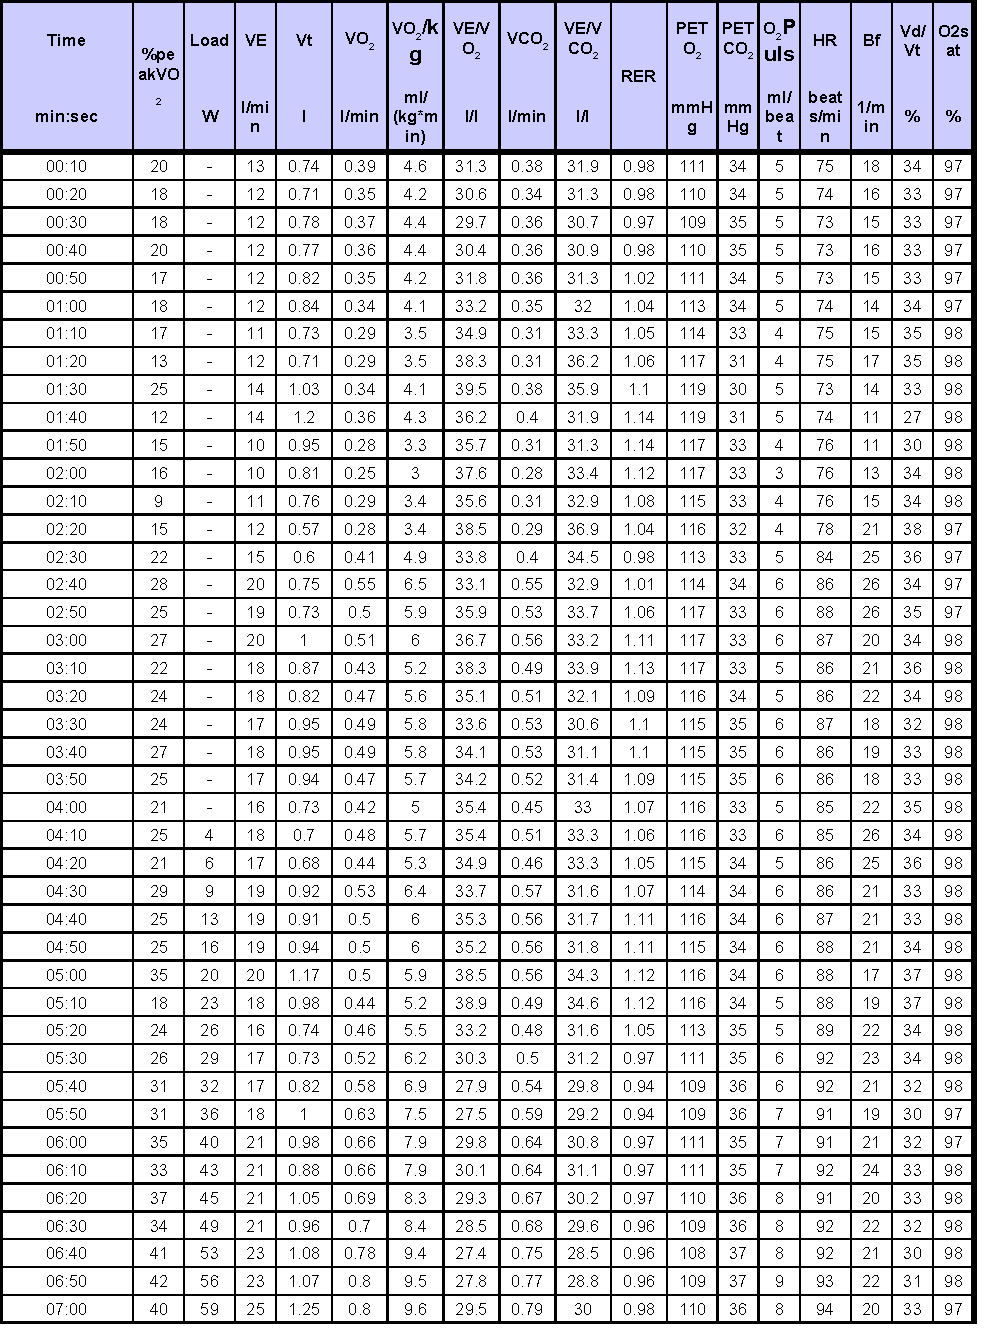
\includegraphics[width=\textwidth,page=1]{Figures/cpet_9p_rawdata.pdf}
\end{figure}
\begin{figure}
	\centering
	\caption{Breath-by-breath sample data with values averaged every 10 seconds - Part 2.}
	\includegraphics[width=\textwidth,page=2]{Figures/cpet_9p_rawdata.pdf}
\end{figure}
\setstretch{1.0}
%\input{Appendices/AppendixC}

\addtocontents{toc}{\vspace{2em}} % Add a gap in the Contents, for aesthetics

\backmatter

%----------------------------------------------------------------------------------------
%	BIBLIOGRAPHY
%----------------------------------------------------------------------------------------

\label{Bibliography}

\lhead{\emph{Bibliography}} % Change the page header to say "Bibliography"

%\bibliographystyle{unsrtnat} % Use the "unsrtnat" BibTeX style for formatting the Bibliography
%\printbibliography

\listoftodos

\end{document}  